\documentclass[a4paper,12pt,oneside,openany]{book}	

\usepackage{layout}
\setlength{\textwidth}{15.0 cm}
\setlength{\textheight}{25.0 cm}


\usepackage[english,brazil]{babel}
\usepackage{pagina}	% pagina-padrao
\usepackage{indentfirst}		% for indent
\usepackage[utf8]{inputenc}
\usepackage{graphics,epsfig}
\usepackage{graphics}
\graphicspath{{./figuras/}}
\usepackage{pstricks,pst-node,pst-tree}
\usepackage{alltt}
%\usepackage{makeidx}
%\makeindex
\usepackage[figuresright]{rotating} % for saydways tables and figures
\usepackage{enumerate}			% for configuration of enumerate environment
\usepackage{amsmath}
\usepackage{amssymb}
\usepackage{portland,multirow}
\usepackage{booktabs}
\usepackage{adjustbox}

\setcounter{secnumdepth}{3}	% numeracao ate subsubsecao
\setcounter{tocdepth}{2}	% indice ate subsubsecao

\usepackage{longtable}

%\usepackage{acronym} 
\usepackage{acro}[=v3]
\acsetup{make-links}
\DeclareAcronym{UFRJ}{
	short = {UFRJ},
	long  = {Universidade Federal do Rio de Janeiro},
}

\DeclareAcronym{LPS}{
	short = {LPS},
	long  = {Laboratório de Processamento de Sinais},
}

\DeclareAcronym{ANP}{
	short = {ANP},
	long  = {Agência Nacional do Petróleo, Gás Natural e Biocombustíveis},
}

\DeclareAcronym{PNPB}{
	short = {PNPB},
	long  = {Programa Nacional de Produção e Uso de Biodiesel},
}

\DeclareAcronym{ARIMA}{
	short = {ARIMA},
	short-plural-form = {ARIMAs},
	long  = {Modelo Autoregressivo Integrado de Médias Móveis},
	long-plural-form = {Modelos Autoregressivos Integrados de Médias Móveis},
	foreign = {do inglês \textit{{A}uto{r}egressive {I}ntegrated {M}oving {A}verage Model}},
	foreign-plural-form = {do inglês \textit{{A}uto{r}egressive {I}ntegrated {M}oving {A}verage Model{s}}}
}

\DeclareAcronym{DA-RNN}{
	short = {DA-RNN},
	short-plural-form = {DA-RNNs},
	long  = {Rede Neural Recorrente Baseada em Atenção de Dois Estágios},
	long-plural-form  = {Redes Neurais Recorrentes Baseadas em Atenção de Dois Estágios},
	foreign = {do inglês \textit{{D}ual-Stage {A}ttention-Based {R}ecurrent {N}eural {N}etwork}},
	foreign-plural-form = {do inglês \textit{{D}ual-Stage {A}ttention-Based {R}ecurrents {N}eurals {N}etworks}}
}

\DeclareAcronym{IDLN}{
	short = {IDLN},
	short-plural-form = {IDLNs},
	long  = {Neurônio Crescente Decrescente Linear},
	long-plural-form = {Neurônios Crescentes Decrescentes Lineares},
	foreign = {do inglês \textit{{I}ncreasing-{D}ecreasing {L}inear {N}euron}},
	foreign-plural-form = {do inglês \textit{{I}ncreasing-{D}ecreasing {L}inear {N}eurons}}
}

\DeclareAcronym{IMP}{
	short = {IMP},
	short-plural-form = {IMPs},
	long  = {Perceptron Morfológico Crescente},
	long-plural-form = {Perceptrons Morfológicos Crescentes},
	foreign = {do inglês \textit{{I}ncreasing {M}orphological {P}erceptron}},
	foreign-plural-form = {do inglês \textit{{I}ncreasing {M}orphological {P}erceptrons}}
}

\DeclareAcronym{IPCA}{
	short = {IPCA},
	long  = {Índice Nacional de Preços ao Consumidor Amplo},
}

\DeclareAcronym{LSTM}{
    short = {LSTM},
    short-plural-form = {LSTMs},
    long = {Rede Neural com Memória de Longo e Curto Prazo},
    long-plural-form = {Redes Neurais com Memória de Longo e Curto Prazo},
    foreign = {do inglês \textit{{L}ong {S}hort-{T}erm {M}emory}},
    foreign-plural-form = {do inglês \textit{{L}ong {S}hort-{T}erm {M}emory}}
}


\DeclareAcronym{MAPE}{
	short = {MAPE},
	short-plural-form = {MAPEs},
	long  = {Erro Percentual Absoluto Médio},
	long-plural-form = {Erros Percentuais Absolutos Médios},
	foreign = {do inglês \textit{{M}ean {A}bsolute {P}ercentage {E}rror}},
	foreign-plural-form = {do inglês \textit{{M}ean {A}bsolute {P}ercentage {E}rrors}}
}

\DeclareAcronym{MAE}{
	short = {MAE},
	short-plural-form = {MAEs},
	long  = {Erro Absoluto Médio},
	long-plural-form = {Erros Absolutos Médios},
	foreign = {do inglês \textit{{M}ean {A}bsolute {E}rror}},
	foreign-plural-form = {do inglês \textit{{M}ean {A}bsolute {E}rrors}}
}

\DeclareAcronym{MSE}{
	short = {MSE},
	short-plural-form = {MSEs},
	long  = {Erro Quadrático Médio},
	long-plural-form = {Erros Quadráticos Médios},
	foreign = {do inglês \textit{{M}ean {S}quared {E}rror}},
	foreign-plural-form = {do inglês \textit{{M}ean {S}quared {E}rrors}}
}

\DeclareAcronym{MLP}{
	short = {MLP},
	short-plural-form = {MLPs},
	long  = {Perceptron Multicamadas},
	long-plural-form = {Perceptrons Multicamadas},
	foreign = {do inglês \textit{{M}u{l}tilayer {P}erceptron}},
	foreign-plural-form = {do inglês \textit{{M}ulti{l}ayer {P}erceptrons}}
}

\DeclareAcronym{N-Linear}{
	short = {N-Linear},
	long  = {Linear Normalizado},
	foreign = {do inglês \textit{{N}ormalized {Linear}}},
}

\DeclareAcronym{NARX}{
	short = {NARX},
	short-plural-form = {NARXs},
	long  = {Rede Neural Autoregressiva Não-linear com Entradas Exógenas},
	long-plural-form = {Redes Neurais Autoregressivas Não-lineares com Entradas Exógenas},
	foreign = {do inglês \textit{{N}onlinear {A}uto{r}egressive E{x}ogenous Model}},
	foreign-plural-form = {do inglês \textit{{N}onlinear {A}uto{r}egressive E{x}ogenous Model}}
}

\DeclareAcronym{NLPCA}{
	short = {NLPCA},
	short-plural-form = {NLPCA},
	long  = {Análise de Componentes Principais Não Lineares},
	long-plural-form = {Análises de Componentes Principais Não Lineares},
	foreign = {do inglês \textit{{N}on{l}inear {P}rincipal {C}omponent {A}nalysis}},
	foreign-plural-form = {do inglês \textit{{N}on{l}inear {P}rincipal {C}omponent {A}nalyses}}
}

\DeclareAcronym{NHiTS}{
	short = {NHiTS},
	short-plural-form = {NHiTSs},
	long  = {Interpolação Neural Hierárquica para Previsão de Séries Temporais},
	long-plural-form = {Interpolações Neurais Hierárquicas para Previsão de Séries Temporais},
	foreign = {do inglês \textit{{N}eural {Hi}erarchical Interpolation for {T}ime {S}eries Forecasting}},
	foreign-plural-form = {do inglês \textit{{N}eural {Hi}erarchical Interpolation for {T}ime {S}eries Forecasting}}
}

\DeclareAcronym{PCA}{
	short = {PCA},
	short-plural-form = {PCAs},
	long  = {Análise de Componentes Principais},
	long-plural-form = {Análises de Componentes Principais},
	foreign = {do inglês \textit{{P}rincipal {C}omponent {A}nalysis}},
	foreign-plural-form = {do inglês \textit{{P}rincipal {C}omponent {A}nalyse{s}}}
}

\DeclareAcronym{NLP}{
	short = {NLP},
	short-plural-form = {NLPs},
	long  = {Processamento de Linguagem Natural},
	long-plural-form = {Processamentos de Linguagem Natural},
	foreign = {do inglês \textit{{N}atural {L}anguage {P}rocessing}},
	foreign-plural-form = {do inglês \textit{{N}atural {L}anguage {P}rocessings}}
}

\DeclareAcronym{ReLU}{
	short = {ReLU},
	short-plural-form = {ReLUs},
	long  = {Unidade Linear Retificada},
	long-plural-form = {Unidades Lineares Retificadas},
	foreign = {do inglês \textit{{Re}ctified {L}inear {U}nit}},
	foreign-plural-form = {do inglês \textit{{Re}ctified {L}inear {U}nits}}
}

\DeclareAcronym{RMSE}{
	short = {RMSE},
	short-plural-form = {RMSes},
	long  = {Raiz do Erro Quadrático Médio},
	long-plural-form = {Raízes do Erro Quadrático Médio},
	foreign = {do inglês \textit{{R}oot {M}ean {S}quared {E}rror}},
	foreign-plural-form = {do inglês \textit{{R}oot {M}ean {S}quared {E}rrors}}
}

\DeclareAcronym{RNA}{
	short = {RNA},
	short-plural-form = {RNAs},
	long  = {Rede Neural Artificial},
	long-plural-form = {Redes Neurais Artificiais},
}

\DeclareAcronym{RNN}{
	short = {RNN},
	short-plural-form = {RNNs},
	long  = {Rede Neural Recorrente},
	long-plural-form = {Redes Neurais Recorrentes},
	foreign = {do inglês \textit{{R}ecurrent {N}eural {N}etwork}},
	foreign-plural-form = {do inglês \textit{{R}ecurrent {N}eural {N}etworks}}
}

\DeclareAcronym{RW}{
	short = {RW},
	short-plural-form = {RWs},
	long  = {Passeio Aleatório},
	long-plural-form = {Passeios Aleatórios},
	foreign = {do inglês \textit{{R}andom {W}alk}},
	foreign-plural-form = {do inglês \textit{{R}andom {W}alks}}
}

\DeclareAcronym{SLE}{
	short = {SLE},
	short-plural-form = {SLEs},
	long  = {Erro Quadrado Logarítmico},
	long-plural-form = {Erros Quadrados Logarítmicos},
	foreign = {do inglês \textit{{S}quared {L}ogarithmic {E}rror}},
	foreign-plural-form = {do inglês \textit{{S}quared {L}ogarithmic {E}rrors}}
}

\DeclareAcronym{THEIL}{
	short = {THEIL},
	short-plural-form = {THEILs},
	long  = {Estatística U de Theil},
	long-plural-form = {Estatísticas U de Theil},
}

\DeclareAcronym{GPU}{
	short = {GPU},
	short-plural-form = {GPUs},
	long  = {Unidade de Processamento Gráfico},
	long-plural-form = {Unidades de Processamento Gráfico},
	foreign = {do inglês \textit{{G}raphics {P}rocessing {U}nit}},
	foreign-plural-form = {do inglês \textit{{G}raphics {P}rocessing {U}nits}}
}

\DeclareAcronym{CUDA}{
	short = {CUDA},
	short-plural-form = {CUDAs},
	long  = {Arquitetura de Dispositivo de Computação Unificada},
	long-plural-form = {Arquiteturas de Dispositivo de Computação Unificada},
	foreign = {do inglês \textit{{C}ompute {U}nified {D}evice {A}rchitecture}},
	foreign-plural-form = {do inglês \textit{{C}ompute {U}nified {D}evice {A}rchitectures}}
}

\DeclareAcronym{CPU}{
	short = {CPU},
	short-plural-form = {CPUs},
	long  = {Unidade de Processamento Central},
	long-plural-form = {Unidades de Processamento Central},
	foreign = {do inglês \textit{{C}entral {P}rocessing {U}nit}},
	foreign-plural-form = {do inglês \textit{{C}entral {P}rocessing {U}nits}}
}

\DeclareAcronym{OSI}{
	short = {OSI},
	short-plural-form = {OSIs},
	long  = {Iniciativa de código aberto},
	long-plural-form = {Iniciativas de código aberto},
	foreign = {do inglês \textit{{O}pen {S}ource {I}nitiative}},
	foreign-plural-form = {do inglês \textit{{O}pen {S}ource {I}nitiatives}}
}


\usepackage{consts}
\usepackage{datetime}
\usepackage{hyperref}

\usepackage{subcaption}




\begin{document}

\frontmatter
\thispagestyle{empty}

\newdate{currentdate}{\documentDay}{\documentMonth}{\documentYear}

\newdateformat{monthyeardate}{%
	\ifcase\THEMONTH
	\or Janeiro%
	\or Fevereiro%
	\or Março%
	\or Abril%
	\or Maio%
	\or Junho%
	\or Julho%
	\or Agosto%
	\or Setembro%
	\or Outubro%
	\or Novembro%
	\or Dezembro%
	\fi
	\space de \THEYEAR%
}


\includegraphics[width=0.25\textwidth]{Poli.eps}
\vfill

\begin{center}
	\large{\MakeUppercase{\documentTitle}}\\
	\vspace{2cm}
	\large{\myName}\\
\end{center}
\vspace{3cm}
\hspace{7cm}
\hfill \parbox{8.0cm}{Projeto de Graduação apresentado ao Curso de Engenharia Eletrônica e de Computação da Escola Politécnica, Universidade Federal do Rio de Janeiro, como parte dos requisitos necessários à obtenção do título de Engenheiro.\\}
\vspace{2cm}
\hfill \parbox{8.0cm}{Orientador: \orientador} \\
\vspace{2cm}
\begin{center}
	\documentPlace

	\monthyeardate\displaydate{currentdate}

\end{center}




\pagebreak


\begin{center}
	\large{\MakeUppercase{\documentTitle}}\\
	\vspace{1cm}
	\large{\myName}\\
\end{center}
\vspace{2cm}
PROJETO DE GRADUAÇÃO SUBMETIDO AO CORPO DOCENTE DO CURSO DE ENGENHARIA ELETRÔNICA E DE COMPUTAÇÃO DA ESCOLA POLITÉCNICA DA UNIVERSIDADE FEDERAL DO RIO DE JANEIRO COMO PARTE DOS REQUISITOS NECESSÁRIOS PARA A OBTENÇÃO DO GRAU DE ENGENHEIRO ELETRÔNICO E DE COMPUTAÇÃO

\vspace{1cm}
Autor:
\vspace{0.5cm}
\begin{flushright}
    \parbox{10cm}{
        \centering
        \vspace{-1cm} % Ajuste o espaço entre a imagem e a linha
        
\includegraphics[height=1cm]{assinatura.png} \\ % Substitua "assinatura.png" pelo caminho da sua imagem
        \vspace{-0.8cm} % Ajuste o espaço entre a imagem e a linha
        \hrulefill

        \vspace{-0.375cm} % Ajuste o espaço entre a linha e o texto
        \centering{\myName}
		\vspace{0.1cm}
		}
\end{flushright}


Orientador:
\vspace{0.5cm}
\begin{flushright}
	\parbox{10cm}{
		\hrulefill

		\vspace{-.375cm}
		\centering{Prof. \orientador, D. Sc.}

		\vspace{0.1cm}
	}
\end{flushright}

Examinador:
\vspace{0.5cm}
\begin{flushright}
	\parbox{10cm}{
		\hrulefill

		\vspace{-.375cm}
		\centering{Prof. José Gabriel Rodriguez Carneiro Gomes, Ph. D.}

		\vspace{0.1cm}
	}
\end{flushright}

Examinador:
\vspace{0.5cm}
\begin{flushright}
	\parbox{10cm}{
		\hrulefill

		\vspace{-.375cm}
		\centering{Kriseida Carmen Portella Guedelha Alekseev, D. Sc.}

		\vspace{0.1cm}
	}
\end{flushright}

Examinador:
\vspace{0.5cm}
\begin{flushright}
	\parbox{10cm}{
		\hrulefill

		\vspace{-.375cm}
		\centering{Prof. Natanael Nunes de Moura Júnior, D. Sc.}

		\vspace{0.1cm}
	}
\end{flushright}


\vfill


\begin{center}
	\documentPlace

	\monthyeardate\displaydate{currentdate}

\end{center}


\pagebreak

% Declaracao
\begin{center}
	Declaração de Autoria e de Direitos
\end{center}

\vspace{0.5cm}

Eu, \emph{\myName} CPF \emph{\myCpf}, autor da monografia \emph{\documentTitle}, subscrevo para os devidos fins, as seguintes informações:\\
1. O autor declara que o trabalho apresentado na disciplina de Projeto de Graduação da Escola Politécnica da UFRJ é de sua autoria, sendo original em forma e conteúdo.\\
2. Excetuam-se do item 1. eventuais transcrições de texto, figuras, tabelas, conceitos e idéias, que identifiquem claramente a fonte original, explicitando as autorizações obtidas dos respectivos proprietários, quando necessárias.\\
3. O autor permite que a UFRJ, por um prazo indeterminado, efetue em qualquer mídia de divulgação, a publicação do trabalho acadêmico em sua totalidade, ou em parte. Essa autorização não envolve ônus de qualquer natureza à UFRJ, ou aos seus representantes.\\
4. O autor pode, excepcionalmente, encaminhar à Comissão de Projeto de Graduação, a não divulgação do material, por um prazo máximo de 01 (um) ano, improrrogável, a contar da data de defesa, desde que o pedido seja justificado, e solicitado antecipadamente, por escrito, à Congregação da Escola Politécnica.\\
5. O autor declara, ainda, ter a capacidade jurídica para a prática do presente ato, assim como ter conhecimento do teor da presente Declaração, estando ciente das sanções e punições legais, no que tange a cópia parcial, ou total, de obra intelectual, o que se configura como violação do direito autoral previsto no Código Penal Brasileiro no art.184 e art.299, bem como na Lei 9.610.\\
6. O autor é o único responsável pelo conteúdo apresentado nos trabalhos acadêmicos publicados, não cabendo à UFRJ, aos seus representantes,  ou ao(s) orientador(es), qualquer responsabilização/ indenização nesse sentido.\\
7. Por ser verdade, firmo a presente declaração.\\

\vspace{0.5cm}
\begin{flushright}
    \parbox{10cm}{
        \centering
        \vspace{-1cm} % Ajuste o espaço entre a imagem e a linha
        
\includegraphics[height=1cm]{assinatura.png} \\ % Substitua "assinatura.png" pelo caminho da sua imagem
        \vspace{-0.8cm} % Ajuste o espaço entre a imagem e a linha
        \hrulefill

        \vspace{-0.375cm} % Ajuste o espaço entre a linha e o texto
        \centering{\myName}
		\vspace{0.1cm}
		}
\end{flushright}

\pagebreak

% Copyright
\vspace{0.5cm}

UNIVERSIDADE FEDERAL DO RIO DE JANEIRO \\
Escola Politécnica - Departamento de Eletrônica e de Computação \\
Centro de Tecnologia, bloco H, sala H-217, Cidade Universitária \\
Rio de Janeiro - RJ      CEP 21949-900\\
\vspace{0.5cm}
\paragraph{}Este exemplar é de propriedade da Universidade Federal do Rio de Janeiro, que poderá incluí-lo em base de dados, armazenar em computador, microfilmar ou adotar qualquer forma de arquivamento.
\paragraph{}É permitida a menção, reprodução parcial ou integral e a transmissão entre bibliotecas deste trabalho, sem modificação de seu texto, em qualquer meio que esteja ou venha a ser fixado, para pesquisa acadêmica, comentários e citações, desde que sem finalidade comercial e que seja feita a referência bibliográfica completa.
\paragraph{}Os conceitos expressos neste trabalho são de responsabilidade do(s) autor(es).


\pagebreak

% Dedicatória
%\begin{center}
%\textbf{DEDICATÓRIA}
%\end{center}
%      \vspace{0.5cm}

%\paragraph{}Opcional.

%\pagebreak


% Agradecimento
\begin{center}
	\textbf{AGRADECIMENTO}
\end{center}
\vspace{0.5cm}

\paragraph{}Agradeço à Deus, em primeiro lugar, porque acredito que sem ele nada é possível.

\paragraph{}Aos meus pais Helena Dias e Euzimar Sena, pelos conselhos e apoio em todos os momentos da minha vida.

\paragraph{}À minha esposa, Mayara Sena, pela companhia nas idas pro Fundão, por todo o incentivo e por todo apoio no desenvolvimento do trabalho.

\paragraph{}Aos meus amigos da UFRJ, Caroline Coelho, Pedro Lídio, João Pedro, Iuri Veloso e Breno Galves, por permanecerem comigo nos momentos bons e ruins.

\paragraph{}Aos meus supervisores da EPE, Kriseida Alekseev e Dan Gandelman, por me proporcionarem a primeira experiência profissional e por todo o incentivo a seguir carreira acadêmica.

\paragraph{}Ao meu orientador, José de Seixas, por aceitar me orientar e proporcionar a realização desse trabalho.

\paragraph{}Aos professores que gentilmente aceitaram fazer parte da minha banca, Natanael Júnior, José Gabriel e Kriseida Alekseev.

\pagebreak


% Resumo
\begin{center}
	\textbf{RESUMO}
\end{center}
\vspace{0.5cm}

\paragraph{} O biodiesel é um biocombustível renovável produzido de fontes vegetais e animais, desempenha um papel importante na transição energética global. A previsão precisa de seu preço é essencial para otimizar sua produção e comercialização, além de apoiar decisões no mercado de biocombustíveis, como o percentual obrigatório de mistura ao diesel.

\paragraph{} Este trabalho explora a aplicação de Redes Neurais Artificiais (\acsp{RNA}) e modelos estatísticos para prever o preço do biodiesel, aliados a modelos de extração de características, como tendência, ciclos senoidais e sazonais, para melhorar o desempenho das previsões. A pesquisa investiga o uso de diferentes modelos para prever o preço do biodiesel, considerando variáveis como o preço do óleo de soja e os preços de biodiesel por regiões do Brasil. As \acsp{RNA} foram escolhidas pela sua capacidade de modelar padrões não lineares e relações complexas entre essas variáveis.

\paragraph{} Os resultados mostram que as \acsp{RNA} têm bom desempenho na previsão do preço do biodiesel, obtendo medidas de desempenho melhores que os modelos estatísticos. Modelos menos profundos, como \acf{N-Linear} e \acf{MLP}, apresentaram melhor resultado nas previsões em comparação aos mais profundos, sugerindo que abordagens mais simples podem ser mais eficazes para capturar os padrões dinâmicos dos preços do biodiesel. Modelos morfológicos, com \acf{IMP} e \acf{IDLN}, também foram testados, mas não apresentaram desempenho satisfatório nas previsões.
\paragraph{}
\noindent Palavras-Chave: previsão de séries temporais, biodiesel, redes neurais, inteligência artificial, biocombustíveis, sustentabilidade.

\pagebreak


% Abstract
\begin{center}
	\textbf{ABSTRACT}
\end{center}
\vspace{0.5cm}

\paragraph{} Biodiesel is a renewable biofuel produced from plant and animal sources and plays an important role in the global energy transition. Accurately predicting its price is essential to optimize its production and commercialization, in addition to supporting decisions in the biofuel market, such as the mandatory percentage of blending with diesel.

\paragraph{} This work explores the application of Artificial Neural Networks (ANN) and statistical models to predict the price of biodiesel, combined with feature extraction models, such as trends, sinusoidal and seasonal cycles, to improve the performance of the predictions. The research investigates the use of different models to predict the price of biodiesel, considering variables such as the price of soybean oil and biodiesel prices by region of Brazil. ANN were chosen for their ability to model non-linear patterns and complex relationships between these variables.

\paragraph{} The results show that ANNs perform well in predicting biodiesel prices, obtaining better performance measures than statistical models. Shallower models, such as Normalized Linear (\acs{N-Linear}) and Multilayer Perceptron (\acs{MLP}), performed better in predictions compared to deeper ones, suggesting that simpler approaches may be more effective in capturing the dynamic patterns of biodiesel prices.Morphological models, with Increasing-Decreasing Linear Neuron (\acs{IDLN}) and Increasing Morphological Perceptron (\acs{IMP}), were also tested, but did not show satisfactory performance in the predictions.
\paragraph{}
\noindent Key-words: time series forecasting, biodiesel, neural networks, artificial intelligence, biofuels, sustainability.

\pagebreak


% Siglas
\begin{center}
	\textbf{LISTA DE ABREVIATURAS}
\end{center}
\vspace{0.5cm}

%\input{acronyms}
\printacronyms[heading=none]


\pagebreak









% Table of Contents
% ---------------------------------------------------------------
\tableofcontents
% ---------------------------------------------------------------
% Lista de figuras
% ---------------------------------------------------------------
%\cleardoublepage
%\addcontentsline{toc}{chapter}{Lista de Figuras}
\listoffigures
% ---------------------------------------------------------------
% Lista de Tabelas
% ---------------------------------------------------------------
%\cleardoublepage
%\addcontentsline{toc}{chapter}{Lista de Tabelas}
\listoftables

\mainmatter
\cleardoublepage
% ---------------------------------------------------------------
% Chapter 1 - Introdução
% ---------------------------------------------------------------
\chapter{Introdução}
\label{cap1}
\paragraph{} As séries temporais são conjuntos de observações coletadas em intervalos regulares e com dependências adjacentes, refletindo o comportamento histórico de um evento ao longo do tempo \cite{box2016time}. A previsão dessas séries é importante para antecipar eventos futuros, como preços de ações e demanda de energia \cite{hyndman2018forecasting, Yasin23}. No entanto, muitas séries temporais não são sistemas invariantes no tempo, sendo influenciadas por mudanças estruturais e fatores externos \cite{maniezo2022serie}. Por isso, modelos avançados são necessários para lidar com essas variações e fatores dinâmicos, buscando uma maior consistência e acurácia nas previsões.
\paragraph{} A previsão de preços de biodiesel é desafiadora devido às influências econômicas, ambientais e políticas que afetam esse mercado emergente, tornando essencial o uso de técnicas avançadas, como modelos estatísticos e redes neurais, para obter previsões com baixo erro \cite{alves2022desafios}. Além disso, a importância das energias renováveis e biocombustíveis, como o biodiesel, está crescendo na busca por soluções sustentáveis e na desaceleração das mudanças climáticas \cite{energia_renovavel}. A adoção dessas fontes de energia reduz a dependência de combustíveis fósseis e promove uma economia de baixo carbono, destacando a necessidade de previsões de preços confiáveis para apoiar a tomada de decisões no setor.
\paragraph{} Redes neurais são eficazes na previsão de séries temporais porque podem identificar relações não lineares e lineares \cite{haykin2009neural}, adaptando-se a novos dados e mudanças no mercado. Esse potencial permite uma tomada de decisão mais informada para diversas partes interessadas, incluindo produtores e consumidores, contribuindo para uma gestão mais eficiente de estoques e planejamento estratégico.
\paragraph{} Desta forma, a aplicação de modelos avançados de redes neurais na previsão de preços de biodiesel é uma abordagem promissora para melhorar a precisão das previsões. Neste contexto, este trabalho propõe o desenvolvimento de um modelo de previsão de preços de biodiesel utilizando redes neurais, de modo a fornecer uma ferramenta confiável e precisa para antecipar as variações de preços nesse mercado em constante evolução.

\section{Tema e Delimitação}

\paragraph{} O tema deste trabalho é a previsão da série temporal de Preços do Biodiesel \cite{biodiesel24}.
\paragraph{} Neste sentido, o problema a ser resolvido é o treinamento do modelo com uma série temporal curta de preços de Biodiesel e as séries correlatas do Óleo de Soja, a fim de prever os preços futuros com precisão e confiabilidade.
\paragraph{} Este trabalho se limitará a uma previsão por um período curto do preço do biodiesel no Brasil, aproximadamente 3 meses. Por se tratar de um mercado em desenvolvimento ainda não há dados suficientes para uma previsão mais longa. Serão utilizados conjuntos de dados públicos do Biodiesel no Brasil \cite{biodiesel24} e do Óleo de Soja no Banco Mundial \cite{worldbank2024}.


\section{Motivação e Justificativa}

\paragraph{} O aumento das concentrações de \(CO_2\) na atmosfera é um dos principais fatores responsáveis pelas mudanças climáticas e pelo aquecimento global. As emissões de gases de efeito estufa provenientes da queima de combustíveis fósseis têm impactos graves no meio ambiente, incluindo o derretimento das calotas polares, o aumento do nível do mar e eventos climáticos extremos. Diante desse cenário, a busca por alternativas sustentáveis e menos poluentes, como os biocombustíveis, torna-se essencial para mitigar os efeitos adversos dessas emissões e promover uma transição para fontes de energia mais limpas.
\paragraph{} O uso de um biocombustível pode contribuir para a redução das emissões de \(CO_2\). A previsão de preços de biodiesel apresenta um desafio complexo devido ao seu comportamento dinâmico e às influências de fatores econômicos, ambientais e políticos. O mercado de biodiesel, ainda em desenvolvimento, é sujeito a variáveis que afetam tanto a oferta quanto a demanda, além de possuir poucos dados para treinamento, tornando as previsões de preços uma tarefa complexa.
\paragraph{} As redes neurais oferecem uma abordagem eficaz e robusta para enfrentar esses problemas. Ao analisar grandes volumes de dados e identificar padrões complexos, essas técnicas avançadas podem fornecer previsões mais precisas e confiáveis. A utilização de redes neurais no desenvolvimento de modelos preditivos para o mercado de biodiesel pode facilitar a tomada de decisões estratégicas, como a otimização de estoques e o planejamento de investimentos, além de ajudar na adaptação às variações do mercado.
\paragraph{} Em resumo, a aplicação de redes neurais na previsão de preços de biodiesel não só contribui para uma análise mais detalhada e precisa das variações de preços, mas também apoia a transição para fontes de energia mais sustentáveis. Dessa forma, a pesquisa contribui para uma melhor compreensão do mercado de biodiesel e para o desenvolvimento de estratégias mais eficientes que apoiem a redução das emissões de \(CO_2\) e a promoção de alternativas energéticas sustentáveis.

\section{Objetivos}

\paragraph{} O objetivo deste trabalho é desenvolver um modelo de previsão de preços de biodiesel usando redes neurais para fornecer uma ferramenta confiável e precisa. Essa abordagem visa antecipar variações de preços em um mercado em evolução, ajudando na otimização de decisões estratégicas e na melhoria da gestão no setor de energia renovável.
\paragraph{} O objetivo geral é, então, desenvolver um modelo de previsão de preços de biodiesel utilizando redes neurais em um período limitado. Desta forma, tem-se como objetivos específicos: (1) realizar a coleta e análise de dados relevantes, como histórico de preços, indicadores econômicos e valores de matérias primas; (2) desenvolver um modelo de redes neurais capaz de processar esses dados e identificar padrões complexos que influenciam os preços; (3) avaliar e aprimorar o desempenho do modelo por meio de técnicas de otimização de hiperparâmetros e medidas de desempenho; (4) aplicar o modelo desenvolvido para prever os preços futuros.

\section{Método}

\paragraph{} O método adotado neste trabalho consiste em utilizar as séries de preços regionais do biodiesel, juntamente com outras variáveis correlatas. Essas séries temporais passam por uma análise de pré-processamento e, em seguida, são aplicados modelos de Machine Learning e Redes Neurais para realizar a modelagem e previsão dos preços nacionais do biodiesel.

\paragraph{} Na análise de séries temporais considera-se que a série é composta por componentes, como heterocedasticidades, tendências, ciclos senoidais, sazonalidades e resíduos, sendo esses componentes considerados independentes uns dos outros. Assim, através da Análise de Componentes Independentes \cite{Faier11}, é realizada uma etapa de pré-processamento dos dados, que inclui a identificação e separação desses componentes. Além disso, é realizada a verificação de outliers \cite{Dantas07}, ou seja, valores discrepantes que possam afetar a qualidade e a interpretação dos dados. Essa etapa tem como objetivo obter uma série temporal mais limpa e preparar para as próximas etapas da análise e modelagem, garantindo a confiabilidade e a integridade dos dados utilizados.


\paragraph{}Após o pré-processamento, os resíduos da série são isolados, os quais geralmente contêm ruídos e relações não lineares entre as variáveis. Para prever esses resíduos, são empregadas redes neurais e outros modelos de Machine Learning, como \ac{RW}, \ac{ARIMA}, \ac{MLP} \cite{haykin2009neural}, \ac{NARX} \cite{haykin1998neural}, \ac{DA-RNN} \cite{zheng2017forecasting}, \ac{IMP} \cite{araujo_morphological_2012}, \ac{IDLN} \cite{Araujo16}, \ac{N-Linear} \cite{DLinear22} e \ac{NHiTS} \cite{NHiTS22}.

\paragraph{}Para o ajuste das redes neurais, são utilizadas medidas de desempenho como \ac{MAPE}, \ac{SLE}, \ac{MAE}, \ac{MSE} e \ac{RMSE}, em conjunto com algoritmos de otimização e ajuste de hiperparâmetros, como GridSearch, RayTune \cite{RayTune18} e Optuna \cite{optuna_2019}, para determinar a melhor arquitetura da rede e obter o melhor ajuste possível. Também são aplicados algoritmos para escolha das principais variáveis, como Matriz de Correlação.

\paragraph{} O êxito deste trabalho está centrado no pré-processamento dos dados e na definição da melhor arquitetura para a rede neural, com o objetivo de minimizar os erros e o custo computacional envolvido. As séries utilizadas no treinamento da rede neural são obtidas a partir de bancos de dados de domínio público, garantindo a disponibilidade e confiabilidade das informações utilizadas.

\section{Materiais}

\begin{itemize}
	\item Cluster do \ac{LPS}, preferencialmente com \ac{GPU};
	\item Python 3.12.4 (\ac{OSI}): \begin{itemize}
		      \item JupyterLab 4.2.2;
		      \item \ac{CUDA} 12.2;
		      \item Pytorch 2.3.1;
		      \item Darts 0.30.0.
	      \end{itemize}
	\item Docker (\ac{OSI});
	\item Séries temporais do histórico de preços: \begin{itemize}
		      \item Biodiesel nacional e regionais;
		      \item Óleo de Soja atual e futuro.
	      \end{itemize}
\end{itemize}

\section{Estrutura do Trabalho}

\paragraph{} O presente trabalho está organizado em 7 capítulos, conforme a seguir:
\paragraph{} \textbf{Capítulo 1 - Introdução: } Reponsável por contextualizar o tema, delimitar o problema, justificar a pesquisa, apresentar os objetivos e o método adotado.
\paragraph{} \textbf{Capítulo 2 - O Biodiesel: } Apresenta uma visão geral sobre o biodiesel, sua importância e impacto no mercado de energia, bem como os desafios e oportunidades associados a esse biocombustível.
\paragraph{} \textbf{Capítulo 3 - Redes Neurais Artificiais: } Introduz as redes neurais artificiais, explicando seus fundamentos teóricos, arquiteturas mais comuns, funcionamento e o processo de aprendizagem, destacando seu uso em problemas de predição e classificação.
\paragraph{} \textbf{Capítulo 4 - Previsão de Séries Temporais: } Discute os conceitos e técnicas de previsão de séries temporais, destacando a importância da análise de dados e modelagem para antecipar eventos futuros.
\paragraph{} \textbf{Capítulo 5 - Descrição do Método: } Apresenta o método adotado para desenvolver o modelo de previsão de preços de biodiesel, incluindo a coleta e análise de dados, o pré-processamento das séries temporais, a modelagem com redes neurais e a avaliação do desempenho do modelo.
\paragraph{} \textbf{Capítulo 6 - Resultados : } Apresenta os resultados obtidos com a aplicação do modelo de previsão de preços de biodiesel, incluindo a análise dos dados, a comparação com outros modelos e a avaliação da precisão das previsões.
\paragraph{} \textbf{Capítulo 7 - Conclusões e Trabalhos Futuros: } Apresenta as conclusões gerais da pesquisa, ressaltando a contribuição do estudo para a área de previsão de preços de biocombustíveis e redes neurais artificiais. Propõe possíveis melhorias no modelo e sugere direções para pesquisas futuras.


% ---------------------------------------------------------------
% Chapter 2 - O Biodiesel
% ---------------------------------------------------------------
\chapter{O Biodiesel}
\label{cap2}
\paragraph{} Este capítulo tem como objetivo apresentar uma breve introdução sobre o Biodiesel. Além disso, será descrito seu desenvolvimento no mercado brasileiro.

\paragraph{} O Biodiesel é um biocombustível produzido a partir de fontes renováveis como óleos vegetais e gorduras animais que reagem por meio de transesterificação com um álcool primário. Embora o biodiesel possa ser produzido a partir de várias matérias-primas, no Brasil o óleo de soja é a principal fonte de matéria-prima para a produção de biodiesel \cite{biodiesel_def_anp}, respondendo por mais de 70\% da produção.
\paragraph{} No Brasil, a introdução do biodiesel na matriz energética tem sido uma resposta tanto às questões ambientais quanto à necessidade de diversificação das fontes de energia e colocam o Brasil como referência no ramo de biocombustíveis \cite{biodiesel_esp_anp}.

\section{Vantagens em Relação ao Óleo Diesel}
\paragraph{} A substituição do Óleo Diesel pelo Biodiesel apresenta uma série de vantagens. No ponto de vista ambiental, a queima do Biodiesel B100 não libera Óxidos de Enxofre (\(SO_x\)), que são agentes causadores da chuva ácida, além de ser biodegradável, se decompondo mais rápido que combustíveis fósseis. No que diz respeito à saúde da população, sua queima gera emissões com baixa concentração de Monóxido de Carbono (\(CO\)) \cite{silva2023biodiesel}, que pode causar sérios problemas respiratórios e cardiovasculares. Além disso, pode ser usado em motores a diesel convencionais sem a necessidade de grandes modificações \cite{totalenergies_biodiesel}.
\paragraph{} O biodiesel apresenta uma vantagem significativa em relação à pegada de carbono devido ao seu ciclo de \(CO_2\) relativamente curto. O dióxido de carbono emitido durante a queima do biodiesel é compensado pela fotossíntese das plantas que fornecem as matérias-primas \cite{silva2023biodiesel}, o que contribui para a minimização dos impactos no aquecimento global.
\paragraph{} Em contrapartida, sua produção depende do uso de terras agrícolas \cite{totalenergies_biodiesel} e de produtos da cesta básica, como o óleo de soja \cite{infomoney_cesta_basica}, provocando aumento nos preços. O biodiesel também é mais corrosivo e sujeito a degradação do que os combustíveis fósseis, o que pode provocar problemas em motores mais antigos que ainda possuem componentes feitos de materiais como plásticos, metais e borrachas de origem natural \cite{totalenergies_biodiesel}.

\section{Produção de Biodiesel no Brasil}

\paragraph{}A produção de biodiesel no Brasil começou a ganhar impulso no início dos anos 2000, com a implementação do \ac{PNPB}.

\paragraph{}Segundo a \ac{ANP}, a produção de biodiesel no Brasil alcançou cerca de 7,5 bilhões de litros em 2023 \cite{ANPBoletim12_2023}, em 2024 espera-se produzir 10 bilhões de litros \cite{ANPBoletim01_2024}.

\section{Regulação e Início do Mercado}

\paragraph{} O \ac{PNPB}, criado em 2004, foi o marco inicial para a regulamentação do biodiesel no Brasil. Este programa foi essencial para estabelecer as bases legais e econômicas para a produção e comercialização do biodiesel. Em 2005, foi autorizada a mistura de biodiesel ao diesel, até 2\%. Em 2008, a mistura se tornou obrigatória, em 2\% (B2), aumentando gradualmente ao longo dos anos \cite{biodiesel_def_anp}.
\paragraph{} Inicialmente, as vendas eram exclusivamente por meio de leilões realizados pela \ac{ANP}. A partir de 2021, foi autorizada a compra diretamente com os fornecedores com venda bimestral regulada pela \ac{ANP} \cite{epbr2021}.

\begin{figure}
	\begin{center}
		\parbox[htb]{13.0cm}
		{
			\begin{center}
				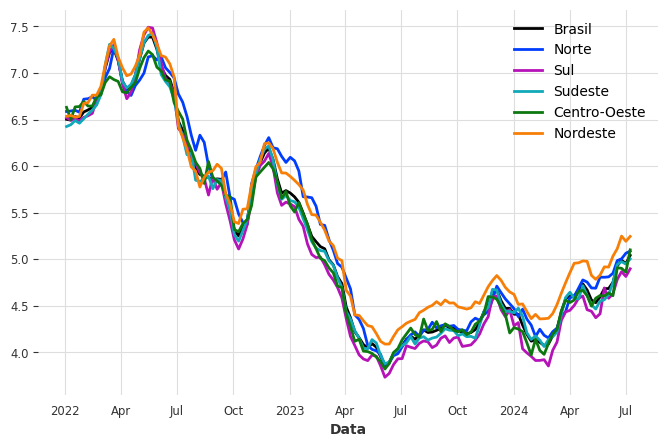
\includegraphics[width=0.8\textwidth]{figuras/biodiesel_price.png}
				\caption{Série de Preços do Biodiesel no Brasil (R\$/litro) a partir de 2022}
				\label{fig:biodiesel_price}
				\text{Fonte: Elaborado pelo autor, baseado em \ac{ANP} \cite{biodiesel24}}
			\end{center}
		}
	\end{center}
\end{figure}

\subsection{Percentuais de Adição no Diesel}

\paragraph{} A mistura obrigatória de biodiesel no diesel tem sido aumentada progressivamente desde sua criação, se adaptando a oferta das matérias primas e ao desenvolvimento das tecnologias de produção.
\paragraph{} Devido à crise de oferta de soja em 2020 aliada ao aumento do \ac{IPCA}, o percentual de mistura foi reduzido de 12\% para 10\% em setembro de 2020 para reduzir os efeitos da crise. Em 2023, o percentual de mistura de biodiesel no diesel volta a subir \cite{g12020} de acordo com o planejamento da \ac{ANP}. Além disso, a recente Lei 14.993, de 2024 \cite{lei14993}, sancionada pelo presidente da república, estabelece novos percentuais crescentes para a mistura de biodiesel no diesel, como parte da estratégia nacional para promover os chamados "combustíveis do futuro" \cite{senadonoticias}. 
\paragraph{} Atualmente, especialistas acreditam que a produção é capaz de atender a demanda de uma mistura de 20\% de biodiesel no óleo diesel e com potencial para chegar a 25\% \cite{canalrural_biodiesel}, ainda longe das projeções da \ac{ANP}, como mostrado na Tabela \ref{tab:mistura_biodiesel}.


\begin{table}[htbp]
	\begin{center}
		\caption{Percentual de Mistura de Biodiesel no Brasil ao Longo do Tempo}
		\label{tab:mistura_biodiesel}
		\begin{tabular}{|c|c|}
	\hline
	\textbf{Período}                       & \textbf{Percentual de Mistura (\%)} \\
	\hline
	01/2005 - 12/2007\textsuperscript{*}   & 2                                   \\
	01/2008 - 06/2008                      & 2                                   \\
	07/2008 - 06/2009                      & 3                                   \\
	07/2009 - 12/2009                      & 4                                   \\
	01/2010 - 06/2014                      & 5                                   \\
	07/2014 - 10/2014                      & 6                                   \\
	11/2014 - 02/2017                      & 7                                   \\
	03/2017 - 02/2018                      & 8                                   \\
	03/2018 - 08/2019                      & 10                                  \\
	09/2019 - 02/2020                      & 11                                  \\
	03/2020 - 08/2020                      & 12                                  \\
	09/2020 - 10/2020\textsuperscript{**}  & 10                                  \\
	11/2020 - 12/2020                      & 11                                  \\
	01/2021 - 02/2021                      & 12                                  \\
	03/2021 - 04/2021                      & 13                                  \\
	05/2021 - 08/2021\textsuperscript{**}  & 10                                  \\
	09/2021 - 10/2021                      & 12                                  \\
	11/2021 - 03/2023\textsuperscript{**}  & 10                                  \\
	04/2023 - 03/2024                      & 12                                  \\
	04/2024 - 02/2025\textsuperscript{***} & 13                                  \\
	03/2025 - 02/2026\textsuperscript{***} & 15                                  \\
	03/2026 - 02/2027\textsuperscript{***} & 16                                  \\
	03/2027 - 02/2028\textsuperscript{***} & 17                                  \\
	03/2028 - 02/2029\textsuperscript{***} & 18                                  \\
	03/2029 - 02/2030\textsuperscript{***} & 19                                  \\
	03/2030\textsuperscript{***} 		   & 20                                 \\
	\hline
\end{tabular}
		\begin{minipage}{\textwidth}
			\footnotesize
			\textsuperscript{*} Percentual de mistura de biodiesel facultativo. \\
			\textsuperscript{**} Queda no percentual obrigatório devido à escassez de soja \cite{g12020}. \\
			\textsuperscript{***} Projeção. \\
		\end{minipage}
		\text{Fonte: \ac{ANP} \cite{biodiesel_esp_anp} e Lei 14.993, de 2024 \cite{lei14993}}
	\end{center}
\end{table}

\subsubsection{Biodiesel 100\% (B100)}

A \ac{ANP} regula o uso experimental do biodiesel B100 através de resoluções específicas. Para utilizar B100 experimentalmente, é necessário obter a prévia anuência da ANP, apresentando um projeto detalhado que especifica o objetivo do experimento, os volumes a serem utilizados, a logística envolvida, os riscos e as medidas de mitigação \cite{ANP910_2022}.

% ---------------------------------------------------------------
% Chapter 3 - Redes Neurais Artificiais
% ---------------------------------------------------------------
\chapter{Redes Neurais Artificiais}
\label{cap3}
\paragraph{} \ac{RNA} é uma classe de modelos de aprendizado de máquina inspirados no funcionamento do cérebro humano, sendo capazes de aprender e tomar decisões com base em amostras apresentados durante o processo de treinamento \cite{haykin1998neural}. A partir dessas amostras, as redes neurais generalizam o aprendizado para dados previamente desconhecidos, permitindo que realizem inferências sobre novos conjuntos de dados.

\paragraph{} As \ac{RNA}s são geralmente estruturadas em três tipos de camadas: camada de entrada, camadas ocultas (ou de processamento) e camada de saída. Essas camadas podem ser organizadas de diversas maneiras, formando topologias específicas que variam de acordo com a aplicação. À medida que os dados de entrada percorrem as camadas da rede, eles são transformados progressivamente por meio de funções de ativação e ajustes sinápticos, que determinam a força das conexões entre os neurônios.

\paragraph{} O ajuste dos pesos sinápticos ocorre durante o processo de treinamento, em que algoritmos de otimização, como o método do gradiente descendente, são utilizados para minimizar o erro entre a saída prevista e a saída desejada. A retropropagação do erro é uma técnica amplamente utilizada para este fim, ajustando os pesos de forma iterativa e eficiente, garantindo a convergência para uma solução ótima.

\paragraph{} Quando uma rede neural recebe um vetor de entrada \(x\), ela realiza cálculos que geram uma saída \(y\), de acordo com a Equação \ref{eq:nn}:

\begin{equation}
	y = f(Wx + b)
	\label{eq:nn}
\end{equation}

\paragraph{} Nesta equação, \(W\) representa a matriz de pesos sinápticos da rede, \(b\) corresponde ao vetor de viés ajustado durante o treinamento, e \(f\) é a função de ativação, responsável por introduzir não linearidades no modelo. A saída \(y\) é, portanto, o resultado final do processamento, obtido após a aplicação dessas transformações.

\section{Perceptron de Rosenblatt}

\paragraph{} O Perceptron, introduzido por Rosenblatt, 1958 \cite{rosenblatt1958perceptron}, foi um dos primeiros modelos de rede neural e representa um marco no desenvolvimento da inteligência artificial. Ele foi concebido para realizar tarefas de classificação linear, sendo capaz de separar classes de dados que são linearmente separáveis. O modelo Perceptron é composto por um único neurônio, que processa um conjunto de entradas, cada uma associada a um peso sináptico, e produz uma saída binária com base em uma função de ativação \cite{rosenblatt1958perceptron}.

\paragraph{} O funcionamento do Perceptron é descrito da seguinte forma:

\begin{equation}
	y = \begin{cases}
		1, & \text{se } \sum_{i=1}^{n} w_i x_i + b > 0 \\
		0, & \text{caso contrário}
	\end{cases}
\end{equation}

\paragraph{} Sendo \(x_i\) as entradas do modelo, \(w_i\) os pesos sinápticos associados a cada entrada, \(b\) o viés (bias) do modelo, ajustável durante o treinamento, e \(y\) a saída binária do Perceptron.

\subsection{Limitações e Extensões}

\paragraph{} Embora o Perceptron tenha sido um avanço significativo, ele é limitado a problemas que podem ser separados por uma linha reta (ou hiperplano no caso de dimensões superiores), ou seja, dados que são linearmente separáveis. Em 1969, Minsky e Papert \cite{minsky1969perceptrons} demonstraram que o Perceptron era incapaz de resolver problemas como o XOR, que não são linearmente separáveis. Essa limitação levou à introdução de arquiteturas mais complexas, como o \ac{MLP}, que supera essa deficiência ao incorporar camadas ocultas e ativação não linear \cite{minsky1969perceptrons}.

\paragraph{} O Perceptron de Rosenblatt foi fundamental para o desenvolvimento posterior de redes neurais e permanece como um conceito básico no aprendizado de máquina.

\paragraph{} O treinamento do Perceptron utiliza uma regra de aprendizado simples e eficiente, conhecida como regra do Perceptron \cite{rosenblatt1958perceptron}. Para cada amostra de treinamento, os pesos são ajustados de acordo com o erro entre a saída prevista e a saída desejada:

\begin{equation}
	w_{i}(t+1) = w_{i}(t) - \eta \frac{\partial E}{\partial w_{i}(t)}
\end{equation}
\paragraph{} Sendo \(w_{i}(t)\) o peso sináptico do neurônio \(i\) no instante \(t\), \(\eta\) a taxa de aprendizado, que controla o tamanho do passo de ajuste e\(\frac{\partial E}{\partial w_{i}(t)}\) o gradiente do erro em relação ao peso.

\paragraph{} Essa regra de atualização ajusta os pesos para reduzir o erro de classificação em cada iteração.

\section{Treinamento de Redes Neurais}

\paragraph{} O treinamento das redes neurais consiste na apresentação dos dados de entrada, acompanhados das respectivas saídas desejadas (supervisionado), ou simplesmente dos dados de entrada no caso de aprendizagem não supervisionada. Durante o treinamento, o objetivo principal é minimizar a função de perda, que avalia  as saídas previstas pela rede com base nas saídas reais.

\paragraph{} O algoritmo mais comum para esse ajuste é o gradiente descendente, que atualiza os pesos sinápticos conforme a direção de maior declínio do erro. Métodos como o gradiente estocástico, Adam e RMSprop são variações amplamente utilizadas, aprimorando o desempenho em diferentes cenários.

\subsection{Retropropagação}

\paragraph{} A retropropagação  é o algoritmo mais utilizado para o treinamento de redes neurais supervisionadas. Introduzido por Rumelhart et al, 1986 \cite{rumelhart1986learning}, esse algoritmo ajusta os pesos sinápticos da rede para minimizar o erro entre a saída prevista e a saída desejada, utilizando o gradiente descendente.

\paragraph{} A retropropagação ocorre em duas fases principais, mostradas na Figura \ref{fig:mlp_diagram_backprop} e detalhadas a seguir:

\begin{figure}
	\begin{center}
		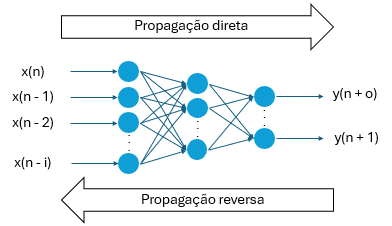
\includegraphics[width=0.8\textwidth]{figuras/mlp_diagram_backprop.png}
		\caption{Diagrama da \acs{MLP} nas fases de retropropagação}
		\label{fig:mlp_diagram_backprop}
		\text{Fonte: Elaborado pelo autor, baseado em \cite{haykin1998neural, rumelhart1986learning}}
	\end{center}
\end{figure}

\begin{itemize}
	\item \textbf{Fase de propagação direta}: Os dados de entrada são propagados pela rede, camada por camada, até que a saída seja calculada. Esta saída é então comparada com o valor esperado, e o erro é calculado com base em uma função de perda, como o \ac{MSE} ou a entropia cruzada.
	\item \textbf{Fase de propagação reversa}: O erro calculado é retropropagado da camada de saída para as camadas anteriores, ajustando os pesos sinápticos de acordo com o gradiente do erro em relação a cada peso. O objetivo é reduzir o erro a cada iteração, tornando o modelo mais preciso.
\end{itemize}

\paragraph{} A atualização dos pesos é dada pela seguinte equação:

\begin{equation}
	w_{ij}(t+1) = w_{ij}(t) - \eta \frac{\partial F_o}{\partial w_{ij}(t)}
\end{equation}
\paragraph{} Sendo \(w_{ij}(t)\) o peso sináptico entre o neurônio \(i\) e o neurônio \(j\) no instante \(t\), \(\eta\) a taxa de aprendizado, que controla o tamanho do passo de ajuste e \(\frac{\partial F_o}{\partial w_{ij}(t)}\) o gradiente da função objetivo em relação ao peso.

\paragraph{} A retropropagação é eficaz em problemas complexos, permitindo o ajuste eficiente dos parâmetros, mas pode enfrentar desafios como o problema do gradiente desaparecendo, que pode ser mitigado com técnicas como funções de ativação como a \ac{ReLU} e o uso de redes profundas com inicializações adequadas de peso.

\section{Funções de Ativação}

\paragraph{} As funções de ativação são elementos essenciais nas redes neurais, pois introduzem não linearidade no modelo, permitindo que ele aprenda padrões complexos. Entre as funções de ativação mais utilizadas estão:

\begin{itemize}
	\item \textbf{Sigmoide}:
	      \begin{equation}
		      f(x) = \frac{1}{1 + e^{-x}}
	      \end{equation}

	      \paragraph{} É utilizada principalmente em saídas binárias, transformando valores reais em probabilidades entre 0 e 1.
	\item \textbf{\ac{ReLU}}:
	      \begin{equation}
		      f(x) = \max(0, x)
	      \end{equation}

	      \paragraph{} Amplamente utilizada em redes profundas por sua simplicidade e eficiência computacional.
	\item \textbf{Tanh}:
	      \begin{equation}
		      f(x) = \frac{e^x - e^{-x}}{e^x + e^{-x}}
	      \end{equation}

	      \paragraph{} A função tangente hiperbólica, semelhante à sigmoide, mas com saída no intervalo \([-1, 1]\).

	\item \textbf{Softmax}:
	      \begin{equation}
		      f(x_i) = \frac{e^{x_i}}{\sum_{j=1}^{n} e^{x_j}}
	      \end{equation}

	      \paragraph{} Usada em problemas de classificação multiclasse, transformando um vetor de valores em probabilidades.
\end{itemize}


\section{Arquiteturas}

As redes neurais podem assumir diferentes arquiteturas, de acordo com o problema que se busca resolver. A seguir, algumas das principais arquiteturas:

\begin{itemize}

	\item \textbf{\acf{NARX}}: A rede \ac{NARX} é uma arquitetura específica de redes neurais utilizada para modelagem de séries temporais, onde a saída depende não apenas das entradas passadas, mas também de saídas anteriores. Ela é amplamente aplicada em sistemas dinâmicos.

	\item \textbf{\acf{RNN}}: As \acp{RNN} possuem conexões entre os neurônios que permitem o processamento sequencial de dados, tornando-as adequadas para tarefas como modelagem de séries temporais, reconhecimento de fala e tradução automática.

	\item \textbf{\acf{MLP}}: O \ac{MLP} é uma das arquiteturas mais clássicas e simples de redes neurais, composta por múltiplas camadas de neurônios com conexões completas entre si. É utilizado principalmente para problemas de classificação e regressão.

	\item \textbf{Redes Morfológicas}: As redes neurais morfológicas utilizam operadores matemáticos morfológicos no lugar de funções de ativação tradicionais. Elas são especialmente úteis para tarefas de processamento de imagens, onde operações como dilatação e erosão são comuns.

	\item \textbf{Redes Profundas}: As Redes Neurais Profundas são caracterizadas por terem múltiplas camadas ocultas, permitindo a aprendizagem de representações mais complexas e abstratas dos dados. Elas são amplamente utilizadas em áreas como reconhecimento de imagens e processamento de linguagem natural. A profundidade da rede permite a extração de características de alto nível, o que é fundamental para o sucesso em tarefas como a classificação de imagens e tradução automática.

\end{itemize}


% ---------------------------------------------------------------
% Chapter 4 - Previsão de Séries Temporais
% ---------------------------------------------------------------
\chapter{Previsão de Séries Temporais}
\label{cap4}
\paragraph{} Séries temporais, por definição, são conjuntos ordenados de observações, onde cada observação é o valor mensurado de uma variável de interesse em intervalos de tempo específicos \cite{box2016time}. Essas observações são coletadas sequencialmente ao longo do tempo, e a análise de séries temporais envolve a modelagem e previsão dessas observações com base em padrões históricos. A estrutura fundamental de uma série temporal pode ser representada como:

\begin{equation}
	X = \{x_t \in \mathbb{R} \mid t = 1,2,3, \ldots, N\}
\end{equation}

\paragraph{} onde \( x_t \) representa o valor observado no tempo \( t \), e \( N \) é o número total de observações. As séries temporais são amplamente utilizadas para identificar tendências, sazonalidades e ciclos senoidais nos dados, bem como para fazer previsões futuras com base nesses padrões identificados. A análise de séries temporais pode envolver diversas técnicas estatísticas e de aprendizado de máquina, como modelos ARIMA, modelos de suavização exponencial, e métodos baseados em redes neurais. O objetivo é entender a dinâmica dos dados ao longo do tempo e aplicar esse entendimento para prever comportamentos futuros com o maior grau de precisão possível.

\section{Métodos de Decomposição e Normalização}

\subsection{Decomposição dos Dados}
\paragraph{} A decomposição é uma técnica fundamental no processamento de séries temporais, usada para analisar e entender as diferentes componentes que constituem os dados. A decomposição permite separar uma série temporal em componentes distintas \cite{Faier11}, facilitando a análise e a modelagem. A compreensão dessas componentes pode melhorar a precisão dos modelos preditivos.
\paragraph{} A série temporal pode ser definida como:
\begin{equation}
	x_t = T_t + C_t + S_t + R_t
\end{equation}

\paragraph{} onde \( x_t \) representa o valor observado da série temporal no tempo \( t \). A componente \( T_t \) refere-se à tendência, que captura a direção geral ou o padrão de longo prazo nos dados. A tendência pode ser crescente, decrescente ou constante ao longo do tempo e mostra o padrão de longo prazo dos dados. A componente \( C_t \) descreve os ciclos senoidais, que se refere às variações que ocorrem em períodos de tempo mais longos, como ciclos econômicos ou de mercado que não se repetem em intervalos fixos, mas são identificáveis ao longo de vários anos. A componente \( S_t \) corresponde à sazonalidade, que representa variações regulares e previsíveis que ocorrem em intervalos de tempo específicos e fixos, como meses ou estações do ano, refletindo padrões que se repetem regularmente e são previsíveis. Por fim, \( R_t \) é o resíduo, também conhecido como erro ou ruído, que é a parte da série temporal que não é explicada pelas outras componentes. Inclui variações aleatórias e imprevisíveis que não podem ser atribuídas à tendência, ciclos senoidais ou sazonais.

\paragraph{} Compreender essas componentes é essencial para uma análise eficaz de séries temporais, pois permite identificar padrões, prever tendências futuras e ajustar modelos para melhorar sua precisão. Este capítulo explorará detalhadamente esses métodos, suas vantagens e limitações, proporcionando uma base sólida para a aplicação prática da decomposição em séries temporais.

\subsubsection{Remoção de Tendência Linear}
\paragraph{} A remoção de tendência linear (\(T_t\)) é uma técnica utilizada para eliminar a componente linear de um conjunto de dados, permitindo que outros padrões ou características dos dados se destaquem mais claramente. Isso é particularmente útil em séries temporais, onde tendências podem mascarar variações sazonais ou outros comportamentos.
\paragraph{} Um dos métodos aplicados para remover a tendência linear é a regressão linear. Nesse processo, ajusta-se um modelo linear aos dados, representado pela equação:

\begin{equation}
	T = \alpha + \beta X
	\label{eq:linear-regression}
\end{equation}
\paragraph{} onde \(T\) é o valor observado, \(X\) é a variável independente (por exemplo, o tempo), \(\alpha\) é o coeficiente linear, e \(\beta\) é o coeficiente angular que representa a inclinação da tendência. Após ajustar o modelo, a tendência linear é subtraída dos dados originais, resultando em uma série de dados sem tendência, que pode ser analisada ou processada de forma mais eficaz.
\paragraph{} A remoção da tendência é útil em diversas aplicações, como na análise econômica e na meteorologia, onde se busca entender variações mais sutis sem a influência de uma tendência subjacente de longo prazo.

\subsubsection{Remoção de Ciclos Senoidais}
A remoção de ciclos senoidais (\(C_t\)) é uma técnica utilizada para eliminar a componente cíclica de um conjunto de dados, eliminando flutuações que ocorrem em intervalos irregulares e sem uma frequência fixa ao longo do tempo. Essas oscilações são causadas por eventos externos. Para remover a componente cíclica, são utilizadas técnicas como a decomposição clássica e
Análise Espectral \cite{Yasin23}.

\subsubsection{Remoção de Sazonalidade}
A remoção da sazonalidade (\(S_t\)) consiste em remover flutuações regulares e repetitivas nos dados, com padrões que se repetem em determinados intervalos, como mensal, trimestral e anual \cite{Yasin23}. A sazonalidade é normalmente encontrada em combustíveis de acordo com os ciclos de oferta de matéria prima, variação da demanda e outras séries. Esta componente pode ser explicada como a variação do comportamento do consumidor e da oferta ao longo do ano.

\subsubsection{Estimação dos Resíduos}
A estimação dos resíduos (\(R_t\)) é uma etapa complexa na previsão de séries temporais. Essa componente é composta por variações não capturadas pelas remoções de tendência, ciclos senoidais e sazonalidade \cite{Yasin23}. Essa componente necessita de métodos mais avançados para estimação, para isso são usados modelos estatísticos como o \ac{ARIMA} e os modelos neurais.

\subsection{Normalização dos Dados}
\paragraph{} A normalização é um processo fundamental no pré-processamento dos dados. Os métodos de normalização ajustam os valores de um conjunto de dados para que eles sigam uma escala ou distribuição específica, o que pode melhorar o desempenho de algoritmos e facilitar a interpretação dos resultados. Este capítulo mostrará alguns dos métodos de normalização disponíveis na literatura.

\subsubsection{Escalonamento Padrão}
\paragraph{} O escalonamento padrão é uma técnica de normalização que ajusta os valores dos dados para que tenham uma média de 0 e um desvio padrão de 1. Essa abordagem é útil quando se deseja centralizar os dados e ajustar sua dispersão, o que pode melhorar o desempenho de algoritmos de aprendizado de máquina que assumem que os dados são distribuídos de forma normal \cite{vasconcelos2024_distribuicao_normal}. O processo de escalonamento é realizado pela Equação \ref{eq:standard-scaler}, onde \(X_{escalado}\) representa o valor escalonado, \(X\) é o valor original, \(\mu\) é a média do conjunto de dados, e \(\sigma\) é o desvio padrão.

\begin{equation}
	X_{escalado} = \frac{X - \mu}{\sigma}
	\label{eq:standard-scaler}
\end{equation}

\paragraph{} Essa técnica é particularmente útil em algoritmos de aprendizado de máquina como máquinas de vetores de suporte e regressão logística, onde a escala dos dados pode impactar a eficácia do modelo e a velocidade de convergência durante o treinamento.

\subsubsection{Normalização Min-Max}
\paragraph{} A normalização Min-Max é uma técnica utilizada para ajustar os valores dos dados para um intervalo específico, geralmente entre 0 e 1. Essa abordagem é útil quando se deseja manter a relação proporcional entre os valores de entrada, mas reduzir a variação dos dados para um intervalo controlado \cite{geeksforgeeks_scaler}. O processo de normalização é feito pela Equação \ref{eq:normalization-min-max}, onde \(X_{escalado}\) representa o valor normalizado, \(X\) é o valor original, e \(min(X)\) e \(max(X)\) são os valores mínimo e máximo do conjunto de dados, respectivamente.

\begin{equation}
	X_{escalado} = \frac{X - min(X)}{max(X) - min(X)}
	\label{eq:normalization-min-max}
\end{equation}

\paragraph{} Essa técnica é útil em métodos de aprendizado de máquina onde a escala dos dados pode influenciar o desempenho do modelo, como em redes neurais, onde variáveis em diferentes escalas podem levar a uma convergência mais lenta durante o treinamento.


\section{Janelas Temporais}


\paragraph{} Na maioria dos casos, as séries temporais não são estacionárias em todo o período, fatores externos podem alterar o comportamento da série ao longo do tempo, o que torna a extração de características uma tarefa complexa. De forma a minimizar o impacto dessas variações, é adotada a abordagem de janelas temporais.
\paragraph{} A janela temporal é um subconjunto de observações da série temporal defasadas no tempo, possibilitando a extração de características necessárias para a previsão do fenômeno gerador. Diferentes tipos de janelas são utilizados, como TAKENS, SAVIT e GREEN, PI e PETERSON, TANAKA. Essas técnicas buscam identificar os retardos temporais mais relevantes para a previsão dos próximos pontos, definidas pela Equação \ref{eq:sliding_window}.
\begin{equation}
	\hat{y}_{t:t+h} = f(X(t,w)) + r_t
	\label{eq:sliding_window}
\end{equation}

\paragraph{} onde \(\hat{y}_{t:t+h}\) são os valores, para o intervalo de tempo \([t + 1 : t + h]\), \(f\) é a função de
previsão, e \(w\) é o tamanho da janela temporal. A função \(f\) representa o mapeamento entre os pontos do passado \(X(t,w)\). O termo \(r_t\) representa um termo de ruído, que tende a diminuir à medida que \(w\) aumenta \cite{Yasin23}. Desta forma, a escolha adequada do formato e do tamanho da janela temporal é uma etapa importante do processo de previsão, pois influencia diretamente na qualidade das previsões.

\subsection{Janela Deslizante}
\paragraph{} Nesta abordagem, a série temporal é subdividida em janelas de comprimento fixo (\(J\), com \(J < N\)). As janelas são deslocadas ao longo da série com um horizonte de previsão (\(H\)) que define o intervalo entre o início de uma janela e a próxima, conforme ilustrado pela Equação \ref{eq:sliding_window_def}.

\begin{equation}
	j_i = \{x_t \mid t = i, i + 1, i + 2, \ldots, i + J - 1\} \text{ para } i = 1, 1 + H, 1 + 2H, \ldots, N - J + 1
	\label{eq:sliding_window_def}
\end{equation}

Nesta fórmula, \(j_i\) representa a \(i\)-ésima janela, que contém \(J\) observações consecutivas da série temporal, começando na posição \(i\). O parâmetro \(H\) define o deslocamento entre o início de uma janela e a próxima, e as janelas são geradas até o final da série, garantindo que cada janela tenha exatamente \(J\) observações.


\subsection{Janela de Takens}
\paragraph{} Nesta abordagem, a série temporal é subdividida em janelas com comprimento fixo (\(J\), com \(J < N\)). Cada janela é formada a partir de um atraso de tempo \(\tau\) entre as observações, conforme ilustrado pela Equação \ref{eq:takens_window}.

\begin{equation}
	t_i = \{x_{i + k\tau} \mid k = 0, 1, 2, \ldots, J - 1\} \text{ para } i = 1, 2, \ldots, N - J\tau
	\label{eq:takens_window}
\end{equation}

Nesta fórmula, \(t_i\) representa a \(i\)-ésima janela, que contém \(J\) observações da série temporal, começando na posição \(i\) e com um atraso de \(\tau\) entre as observações subsequentes. O parâmetro \(i\) define a posição inicial da janela e é variado até garantir que cada janela tenha exatamente \(J\) observações, com a condição \(i \leq N - J\tau\).


\section{Medidas de Avaliação do Modelo}
\paragraph{} As medidas de avaliação de modelo são utilizadas para quantificar a precisão e a qualidade das previsões feitas por um modelo em relação aos valores reais observados. Essas medidas são essenciais para comparar o desempenho de diferentes modelos e para entender como eles se comportam em diferentes condições de dados.

\subsection{\acf{MAPE}}
\paragraph{} O \ac{MAPE} é uma medida que expressa o erro médio absoluto entre os valores previstos (\(p_t\)) e os valores reais (\(x_t\)) em termos percentuais \cite{oracle_mape}. Ele é definido pela Equação \ref{eq:mape}, onde \(N\) é o número total de observações. O \ac{MAPE} é útil em contextos onde a interpretação do erro em termos de percentual é mais relevante.

\begin{equation}
	MAPE = \frac{1}{N} \sum_{t=1}^{N} \left|\frac{x_t - p_t}{x_t}\right|
	\label{eq:mape}
\end{equation}
\paragraph{} Uma vantagem do \ac{MAPE} é que ele é fácil de interpretar e comparar entre diferentes modelos ou datasets. No entanto, ele pode ser influenciado por valores reais (\(x_t\)) próximos de zero, o que pode resultar em valores extremamente altos para o erro percentual \cite{filho_mape}.

\subsection{\acf{MSE}}
\paragraph{} O \ac{MSE} mede o erro médio ao quadrado entre os valores previstos (\(p_t\)) e os valores reais (\(x_t\)). A fórmula é apresentada na Equação \ref{eq:mse}. O \ac{MSE} é amplamente utilizado porque penaliza erros maiores de forma mais significativa, uma vez que os erros são elevados ao quadrado \cite{datahackers_regressao}.
\begin{equation}
	MSE = \frac{1}{N} \sum_{t=1}^{N} (x_t - p_t)^2
	\label{eq:mse}
\end{equation}
\paragraph{} Essa medida é útil quando se deseja enfatizar grandes desvios nas previsões. No entanto, ela também pode ser sensível a outliers, pois estes contribuem de forma desproporcional para o valor final do \ac{MSE}.

\subsection{\acf{RMSE}}
\paragraph{} O \ac{RMSE} é a raiz quadrada do \ac{MSE}, conforme a Equação \ref{eq:rmse}. Ele mantém as propriedades do \ac{MSE}, mas é expresso na mesma unidade dos valores originais, o que facilita a interpretação \cite{datahackers_regressao}.

\begin{equation}
	RMSE = \sqrt{\frac{1}{N} \sum_{t=1}^{N} (x_t - p_t)^2}
	\label{eq:rmse}
\end{equation}
\paragraph{} O \ac{RMSE} é preferido em situações onde grandes erros são particularmente indesejáveis, e sua interpretação direta em termos das unidades dos dados originais é uma vantagem adicional.

\subsection{\acf{MAE}}
\paragraph{} O \ac{MAE} é a média dos erros absolutos entre as previsões ($p_t$) e os valores reais ($x_t$), conforme mostrado na Equação \ref{eq:mae}. O \ac{MAE} é uma medida intuitiva que mede o erro médio sem considerar a direção do erro (positivo ou negativo) \cite{datahackers_regressao}.

\begin{equation}
	MAE = \frac{1}{N} \sum_{t=1}^{N} \left|x_t - p_t\right|
	\label{eq:mae}
\end{equation}
\paragraph{} Diferente do \ac{MSE} e \ac{RMSE}, o \ac{MAE} não penaliza erros grandes de forma desproporcional, o que o torna uma escolha adequada quando se deseja uma métrica de erro mais equilibrada.

\subsection{\acf{THEIL}}
\paragraph{} O índice de Theil é uma medida utilizada para avaliar a precisão das previsões de um modelo em comparação com um modelo de referência. Ele é particularmente útil para medir a qualidade das previsões em séries temporais e pode ser dividido em dois componentes: \(U_1\) e \(U_2\) \cite{theil_forecast}.

\subsubsection{\(U_1\) de Theil}
\paragraph{} A estatística \( U_1 \) do Índice de Theil avalia a precisão das previsões comparadas com um modelo de referência. A fórmula é dada por:

\begin{equation}
	U_1 = \frac{\sqrt{\frac{1}{N} \sum_{t=1}^{N} (x_t - p_t)^2}}{\sqrt{\frac{1}{N} \sum_{t=1}^{N} x_t^2} + \sqrt{\frac{1}{N} \sum_{t=1}^{N} p_t^2}}
	\label{eq:u1-theil}
\end{equation}
\paragraph{} Quanto mais precisas as previsões, menor o valor da estatística \( U_1 \). A estatística \( U_1 \) é limitada entre 0 e 1, com valores mais próximos de 0 indicando maior precisão de previsão \cite{theil_forecast}.

\subsubsection{\(U_2\) de Theil}
\paragraph{} A estatística \( U_2 \) do Índice de Theil avalia o desempenho do modelo em relação ao modelo ingênuo \cite{theil_forecast}. A fórmula é dada pela equação:
\begin{equation}
	U_2 = \frac{\sqrt{\sum_{t=1}^{N-1} (\frac{P_{t+1} - X_{t+1}}{x_t})^2}}{\sqrt{\sum_{t=1}^{N-1} (\frac{X_{t+1} - X_{t}}{x_t})^2}}
	\label{eq:u2-theil}
\end{equation}
\paragraph{} Os valores de \(U_2\) são classificados em três intervalos:
\begin{itemize}
	\item \(U_2 \in [0, 1)\), o modelo é melhor que o modelo ingênuo
	\item \(U_2 \in (1, \infty)\), o modelo é pior que o modelo ingênuo
	\item \(U_2 = 1\), o modelo é igual ao modelo ingênuo
\end{itemize}

\section{Coeficiente de Hurst}

O Coeficiente de Hurst, denotado por \( H \), é uma medida estatística utilizada para analisar a long-range dependence (dependência de longo alcance) em séries temporais. Originalmente desenvolvido por Harold Edwin Hurst na década de 1950, o coeficiente é uma ferramenta fundamental na análise de dados financeiros, climatológicos e muitos outros campos onde o comportamento temporal é relevante.

\subsection{Definição e Cálculo}

O coeficiente de Hurst varia entre 0 e 1 e fornece informações sobre a tendência e a persistência da série temporal \cite{hurst1951}:

\begin{itemize}
	\item \( \mathbf{H} < \mathbf{0.5} \): A série temporal exibe um comportamento de média reversão, indicando que tendências altas são seguidas por tendências baixas e vice-versa.
	\item \( \mathbf{H} = \mathbf{0.5} \): A série é considerada um \acl{RW}, onde não há dependência temporal.
	\item \( \mathbf{H} > \mathbf{0.5} \): A série exibe um comportamento de persistência, onde altas tendências tendem a ser seguidas por altas e baixas por baixas.
\end{itemize}

Uma forma de calcular o Coeficiente de Hurst é por meio da análise de resíduo de variância (R/S). O procedimento básico envolve os seguintes passos:


\begin{enumerate}
	\item Calcular a média da série temporal \( X(t) \):
	      \[
		      \bar{X} = \frac{1}{N} \sum_{t=1}^{N} X(t)
	      \]
	      onde \( N \) é o número total de observações.
	\item Calcular os desvios acumulados a partir da média:
	      \[
		      Y(t) = \sum_{i=1}^{t} (X(i) - \bar{X})
	      \]
	\item Calcular o desvio padrão dos desvios acumulados em várias escalas \( n \):
	      \[
		      R(n) = \max(Y(t)) - \min(Y(t))
	      \]
	      \[
		      S(n) = \sqrt{\frac{1}{n} \sum_{t=1}^{n} (X(t) - \bar{X})^2}
	      \]
	\item Calcular o R/S:
	      \begin{equation}
		      R/S = \frac{R(n)}{S(n)}
		      \label{eq:hurst}
	      \end{equation}
\end{enumerate}

% ---------------------------------------------------------------
% Chapter 5 - Descrição do Método
% ---------------------------------------------------------------
\chapter{Descrição do Método}
\label{cap5}
\paragraph{} O método aplicado a este trabalho pode ser dividido em 5 etapas principais, se dividindo entre desenvolvimento e teste. Inicia-se pela coleta de dados, a partir de fontes abertas e confiáveis, seguido pela etapa de divisão do conjunto de dados em desenvolvimento e teste, etapas de pré-processamento, onde características principais são extraídas antes do treinamento de um modelo neural e por fim, a avaliação dos modelos no conjunto de desenvolvimento, para a escolha de hiperparâmetros e no conjunto de teste, para avaliar a capacidade de generalização. O diagrama de processamento do método é mostrado na Figura \ref{fig:processamento_diagram} e o método detalhado nas seções a seguir.

\begin{figure}
	\begin{center}
		\begin{center}
			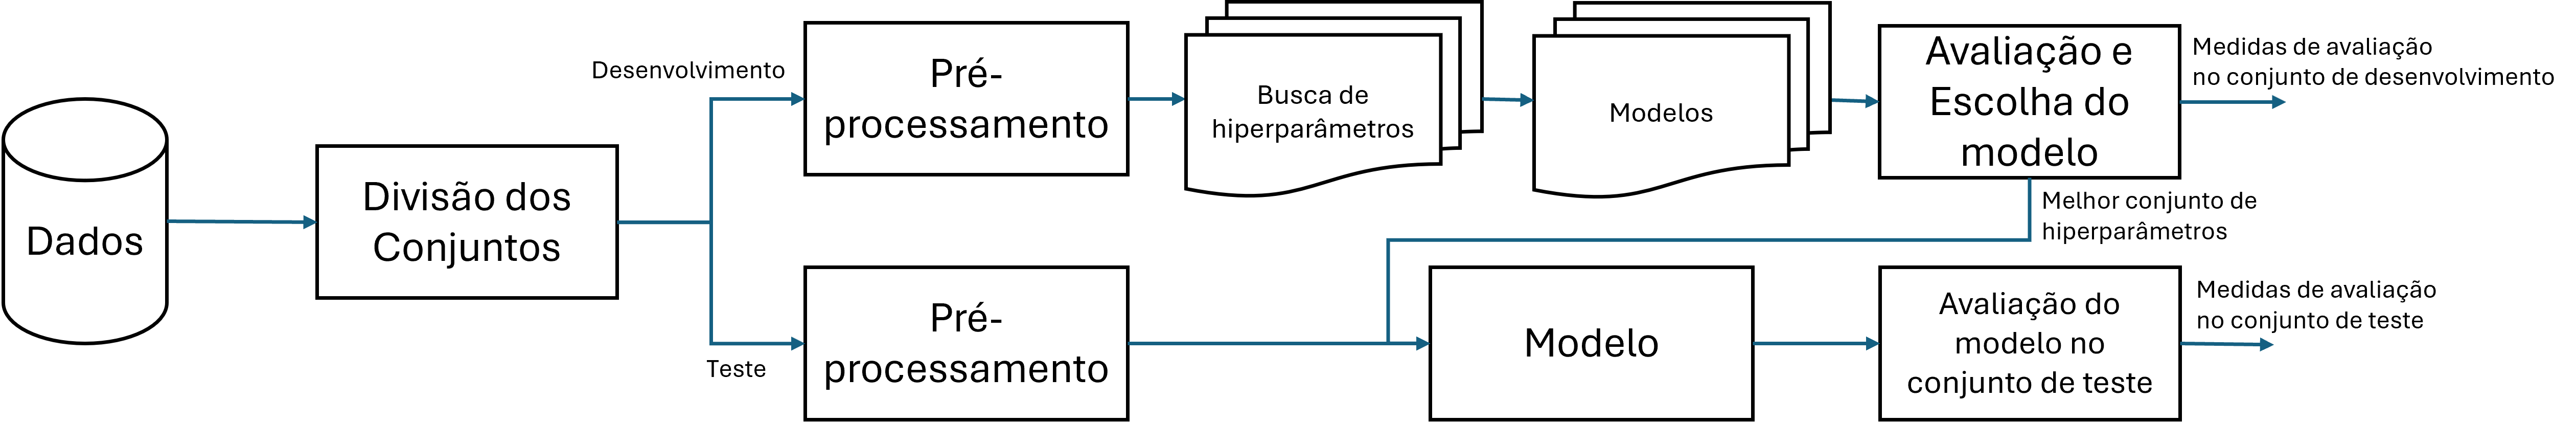
\includegraphics[width=\textwidth]{figuras/processamento_diagram.png}
			\caption{Fluxo de Processamento}
			\label{fig:processamento_diagram}
		\end{center}

	\end{center}
\end{figure}

\section{Coleta de Dados}

\paragraph{} A primeira etapa deste trabalho é a coleta de dados, que é uma etapa importante para a construção de um modelo de previsão. A qualidade dos dados coletados influencia diretamente a qualidade do modelo. Para este trabalho, os dados foram coletados de fontes públicas e confiáveis, como a \ac{ANP} (em conformidade com a Lei de Acesso a Informação \cite{lei12527}), o Banco Mundial e o Index Mundi. O intervalo de tempo escolhido para a análise compreende o período entre janeiro de 2022 e julho de 2023, permitindo a avaliação da série em 2 períodos sazonais para uma previsão no curto prazo.
\paragraph{} Além disso, serão usados como covariáveis passadas as séries de preços do Óleo de Soja Internacional e do Óleo de Soja no Mercado Futuro. Para possibitar uma análise de um período de tempo maior, as séries de preços do Óleo de Soja Internacional e do Óleo de Soja no Mercado Futuro foram coletadas desde 1960 e 1994, respectivamente.
\paragraph{} A seleção das séries temporais foi baseada na disponibilidade de dados históricos e na correlação observada entre elas durante o período de análise, conforme ilustrado na Figura \ref{fig:correlation_matrix}. A alta correlação entre as séries regionais de preços do biodiesel sugere que a inclusão dessas séries no modelo não contribui com informações adicionais relevantes.
\paragraph{} De maneira semelhante, as covariáveis foram escolhidas com base em critérios de correlação. A série de preços do óleo de soja internacional demonstra uma alta correlação com as séries de preços do biodiesel, tornando-a uma candidata promissora para o treinamento do modelo devido à maior disponibilidade de dados. Por outro lado, a série de preços do óleo de soja no mercado futuro também apresenta alta correlação com as séries de preços do biodiesel. No entanto, como essa série tem uma correlação perfeita com a série de preços do óleo de soja internacional, sua inclusão no modelo não adiciona valor informativo adicional.
\paragraph{} Portanto, as séries escolhidas para treinamento do modelo são: Preço do Biodiesel Nacional e Preço do Óleo de Soja Internacional.

\begin{figure}
	\begin{center}
		\begin{center}
			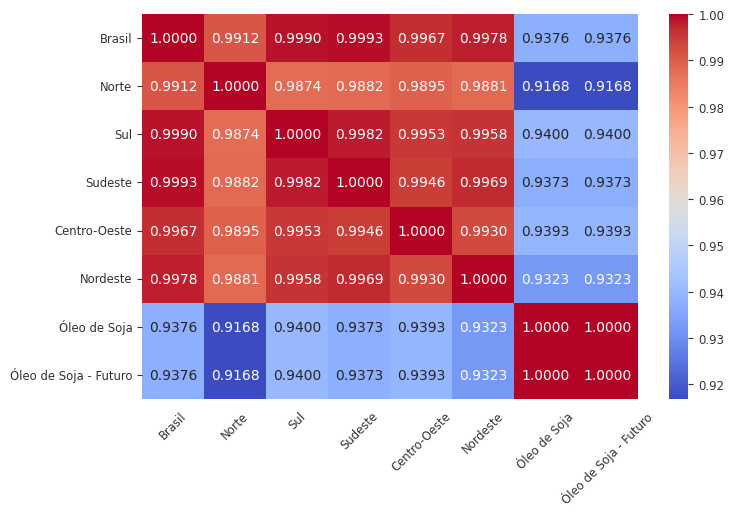
\includegraphics[width=0.8\textwidth]{figuras/correlation_matrix.png}
			\caption{Matriz de Correlação entre as Séries Candidatas (01/2022 - 07/2023)}
			\label{fig:correlation_matrix}
		\end{center}

	\end{center}
\end{figure}

\section{Divisão do Conjunto de Dados}
\paragraph{} Para uma modelagem e avaliação mais eficaz do modelo, os dados foram divididos em dois conjuntos: desenvolvimento e teste, conforme mostrado na Figura \ref{fig:series_conjunto_timeline}.
\paragraph{} O período até julho de 2023 foi alocado para o conjunto de desenvolvimento, que é utilizado para ajustar os hiperparâmetros do modelo e validar sua eficácia. Esse conjunto inclui dados suficientes para observar a dinâmica sazonal e garantir a capacidade de generalização do modelo. Os dados restantes são usados como conjunto de teste, fornecendo uma avaliação final não tendenciosa do modelo com dados que não foram vistos anteriormente. Este modelo de divisão é uma prática recomendada pela literatura para garantir confiabilidade e robustez do modelo de previsão \cite{saha2024}.

\begin{figure}
	\begin{center}
		\begin{center}
			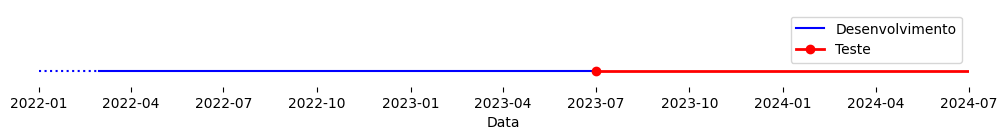
\includegraphics[width=\textwidth]{figuras/series_conjunto_timeline.png}
			\caption{Linha do Tempo da Divisão dos Conjuntos}
			\label{fig:series_conjunto_timeline}
		\end{center}

	\end{center}
\end{figure}


\section{Pré-processamento dos Dados}
\paragraph{} Após a divisão dos conjuntos, é aplicado o processo de pré-processamento. Que pode ser subdividido em em 4 partes principais: Processo de descorrelação, divisão em janelas temporais, extração de características e escalamento do resíduo, como mostrado na Figura \ref{fig:preprocessamento_diagram}.

\begin{figure}
	\begin{center}
		\begin{center}
			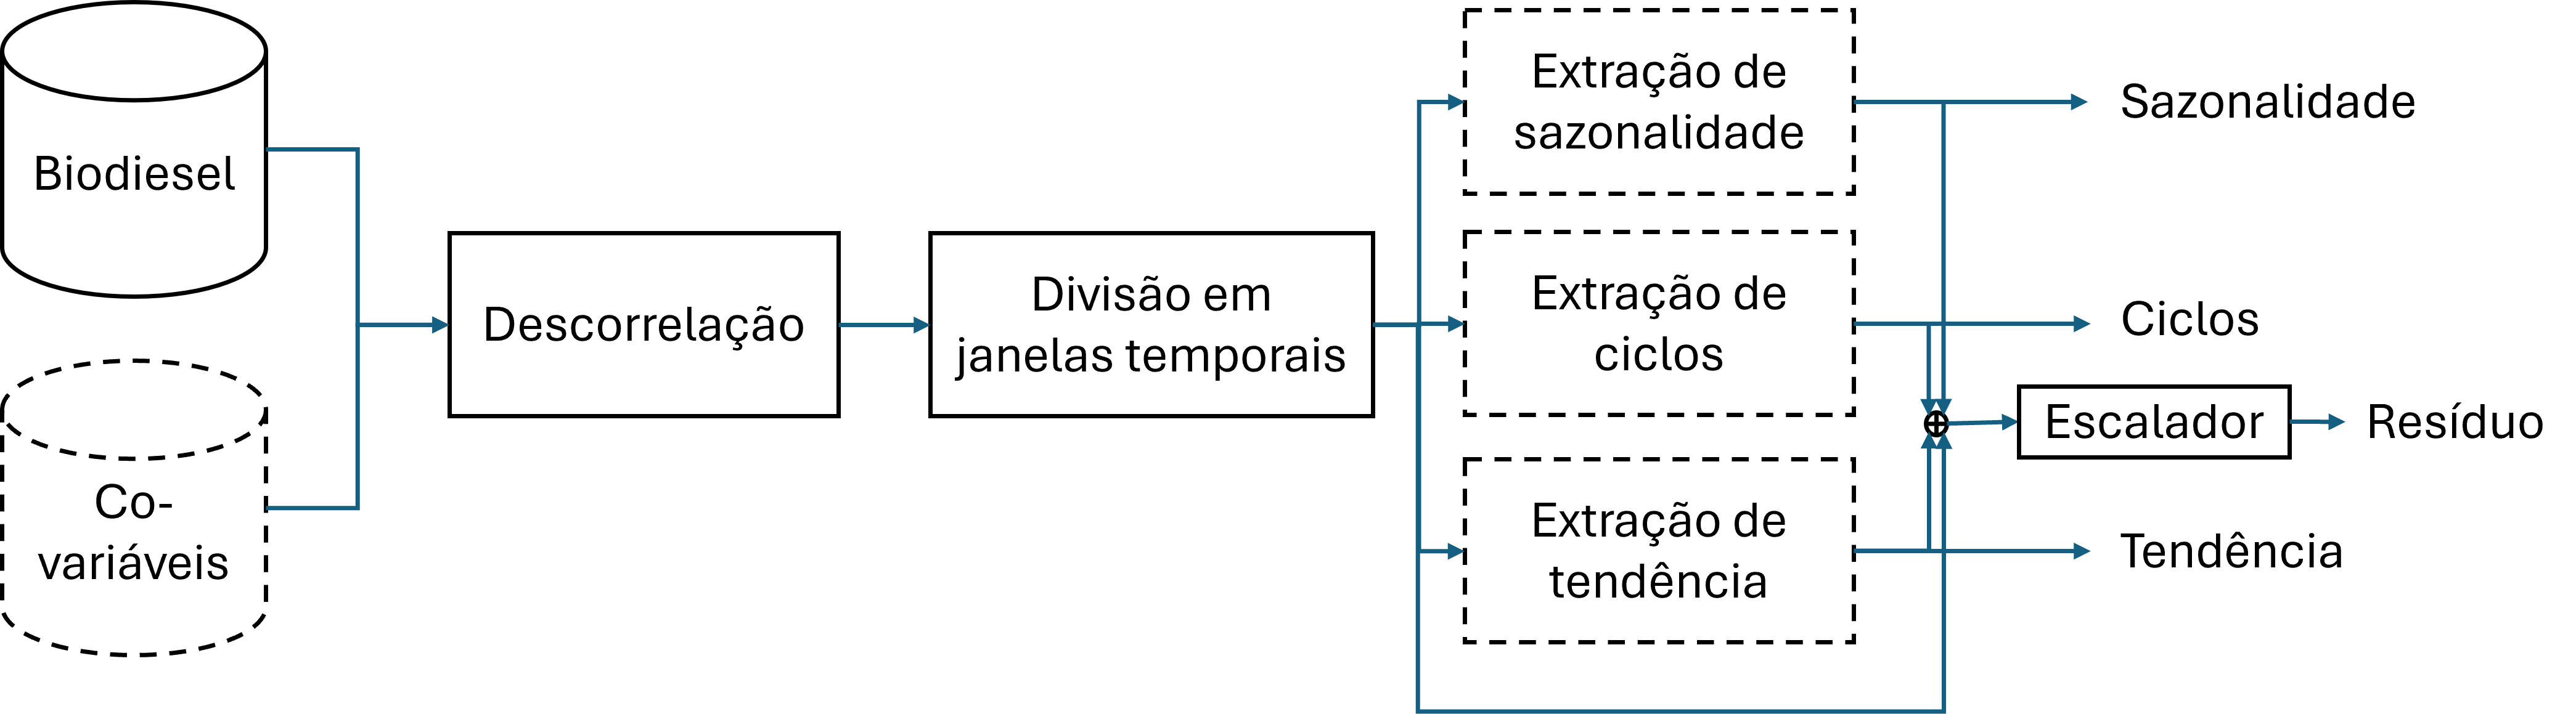
\includegraphics[width=\textwidth]{figuras/preprocessamento_diagram.png}
			\text{---: Obrigatório} \\
			\text{- -:  \space \space \space Opcional}
			\caption{Fluxo de Pré-Processamento}
			\label{fig:preprocessamento_diagram}
		\end{center}

	\end{center}
\end{figure}

\paragraph{} Inicialmente, o conjunto de desenvolvimento foi submetido a uma análise para identificar padrões de sazonalidade e ciclos senoidais. Caso sejam identificados, o tamanho da janela temporal deve ser escolhido de modo a capturar pelo menos 2 observações de cada padrão.
\paragraph{} A verificação da sazonalidade foi realizada por meio da autocorrelação da série temporal. No entanto, a análise não revelou ciclos sazonais completos, conforme ilustrado na Figura \ref{fig:acf_biodiesel}. Além disso, para identificar ciclos senoidais, foi empregada a Transformada Rápida de Fourier (FFT). No entanto, a análise de FFT também não conseguiu identificar ciclos senoidais significativos na série temporal, como mostrado na Figura \ref{fig:fft_biodiesel}. Esses resultados indicam a ausência de padrões sazonais e cíclicos evidentes nos dados analisados.

\paragraph{} A verificação da persistência foi realizada utilizando o Coeficiente de Hurst, conforme descrito na Equação \ref{eq:hurst}. Essa abordagem permite analisar a série temporal para verificar se ela exibe um comportamento de persistência, o que significa que os valores futuros podem ser previstos a partir dos dados passados.
\paragraph{} Com base nessa análise, obteve-se um Coeficiente de Hurst igual a 0,73, constatou-se que a série apresenta um comportamento de persistência, o que implica uma correlação positiva entre os valores atuais e os valores passados. Em outras palavras, quando a série tende a aumentar, as tendências passadas indicam uma probabilidade de continuar subindo, e quando tende a cair, as tendências passadas sugerem uma continuidade desse movimento. Isso reforça a possibilidade de previsão a partir de dados históricos, validando a hipótese de dependência de longo prazo na série temporal.

\begin{figure}
	\begin{center}
		\begin{center}
			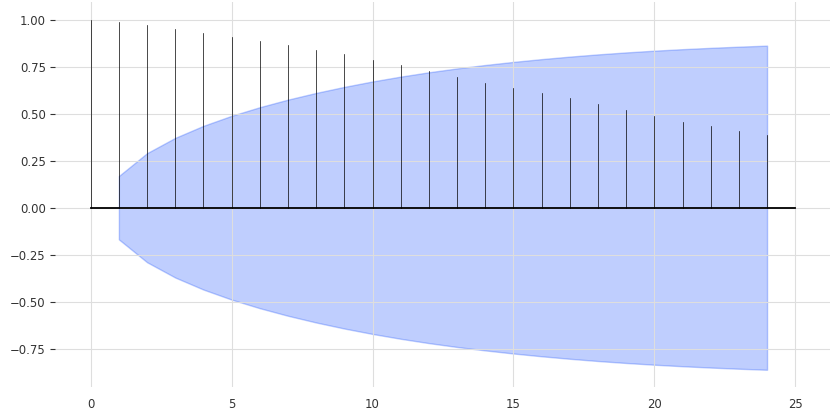
\includegraphics[width=0.8\textwidth]{figuras/acf_biodiesel.png}
			\caption{Autocorrelação da Série de Preços do Biodiesel}
			\label{fig:acf_biodiesel}
		\end{center}

	\end{center}
\end{figure}

\begin{figure}
	\begin{center}
		\begin{center}
			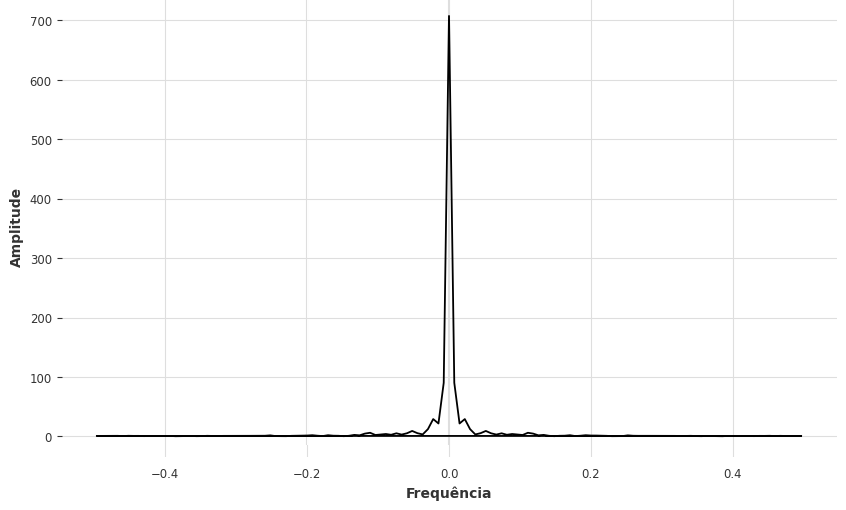
\includegraphics[width=0.8\textwidth]{figuras/fft_biodiesel.png}
			\caption{Frequências de Fourier da Série de Preços do Biodiesel}
			\label{fig:fft_biodiesel}
		\end{center}

	\end{center}
\end{figure}
\paragraph{} Os dados selecionados, o preço do biodiesel nacional e do óleo de soja internacional, foram submetidos a um processo de descorrelação para remover dependências lineares entre as variáveis, como mostrado na matriz de correlação da Figura \ref{fig:correlation_matrix}, removendo os dados da série do óleo de soja internacional no período em que há dados das duas séries, como mostrado na Figura \ref{fig:series_timeline}. Em seguida, os dados foram divididos em dois experimentos distintos. O primeiro experimento considera apenas o preço do biodiesel nacional, enquanto o segundo experimento incorpora tanto o preço do biodiesel quanto o preço do óleo de soja, permitindo a análise do impacto combinado dessas variáveis nos modelos de previsão.

\begin{figure}
	\begin{center}
		\begin{center}
			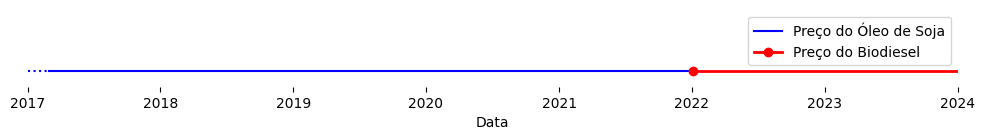
\includegraphics[width=\textwidth]{figuras/series_timeline.png}
			\caption{Linha do Tempo dos Períodos de Disponibilidade das Séries de Biodiesel e Óleo de Soja}
			\label{fig:series_timeline}
		\end{center}

	\end{center}
\end{figure}

\paragraph{} Posteriormente, os dados foram segmentados em janelas temporais, aplicando duas abordagens previamente descritas na fundamentação teórica: (1) Janela Deslizante com sobreposição, que permite capturar a continuidade temporal ao criar séries sobrepostas; e (2) Janela de Takens, que reconstrói o espaço de estados da série temporal a partir de um único sinal, utilizando atrasos específicos para capturar as dinâmicas subjacentes.
\paragraph{} Foram aplicadas duas abordagens distintas para a normalização e decomposição dos dados. Na primeira abordagem, os dados brutos foram normalizados diretamente utilizando a Equação \ref{eq:normalization-min-max}. Na segunda abordagem, os dados foram primeiramente processados para remover a tendência linear, ajustada pela Equação \ref{eq:linear-regression}, resultando em dados residuais. Esses dados residuais foram então normalizados utilizando novamente a Equação \ref{eq:normalization-min-max}.

\section{Treinamento e Avaliação dos Modelos}
\paragraph{} Em seguida, foi realizada a validação cruzada para avaliar o desempenho do modelo de forma mais robusta, assegurando sua eficácia e confiabilidade em diferentes subconjuntos de dados.
\paragraph{} O conjunto de desenvolvimento é dividido em 2 subconjuntos. O conjunto de treinamento, usado para apresentar amostras de pares entrada e saída para o modelo e o conjunto de validação usado para avaliar o modelo em dados que não foram usados para o ajuste de parâmetros, evitando sobreajuste e garantindo a capacidade de generalização. Os conjuntos são divididos com tamanhos diferentes em cada dobra da validação cruzada, conforme mostrado na Figura \ref{fig:validacao_cruzada_teo}.

\begin{figure}
	\begin{center}
		\begin{center}
			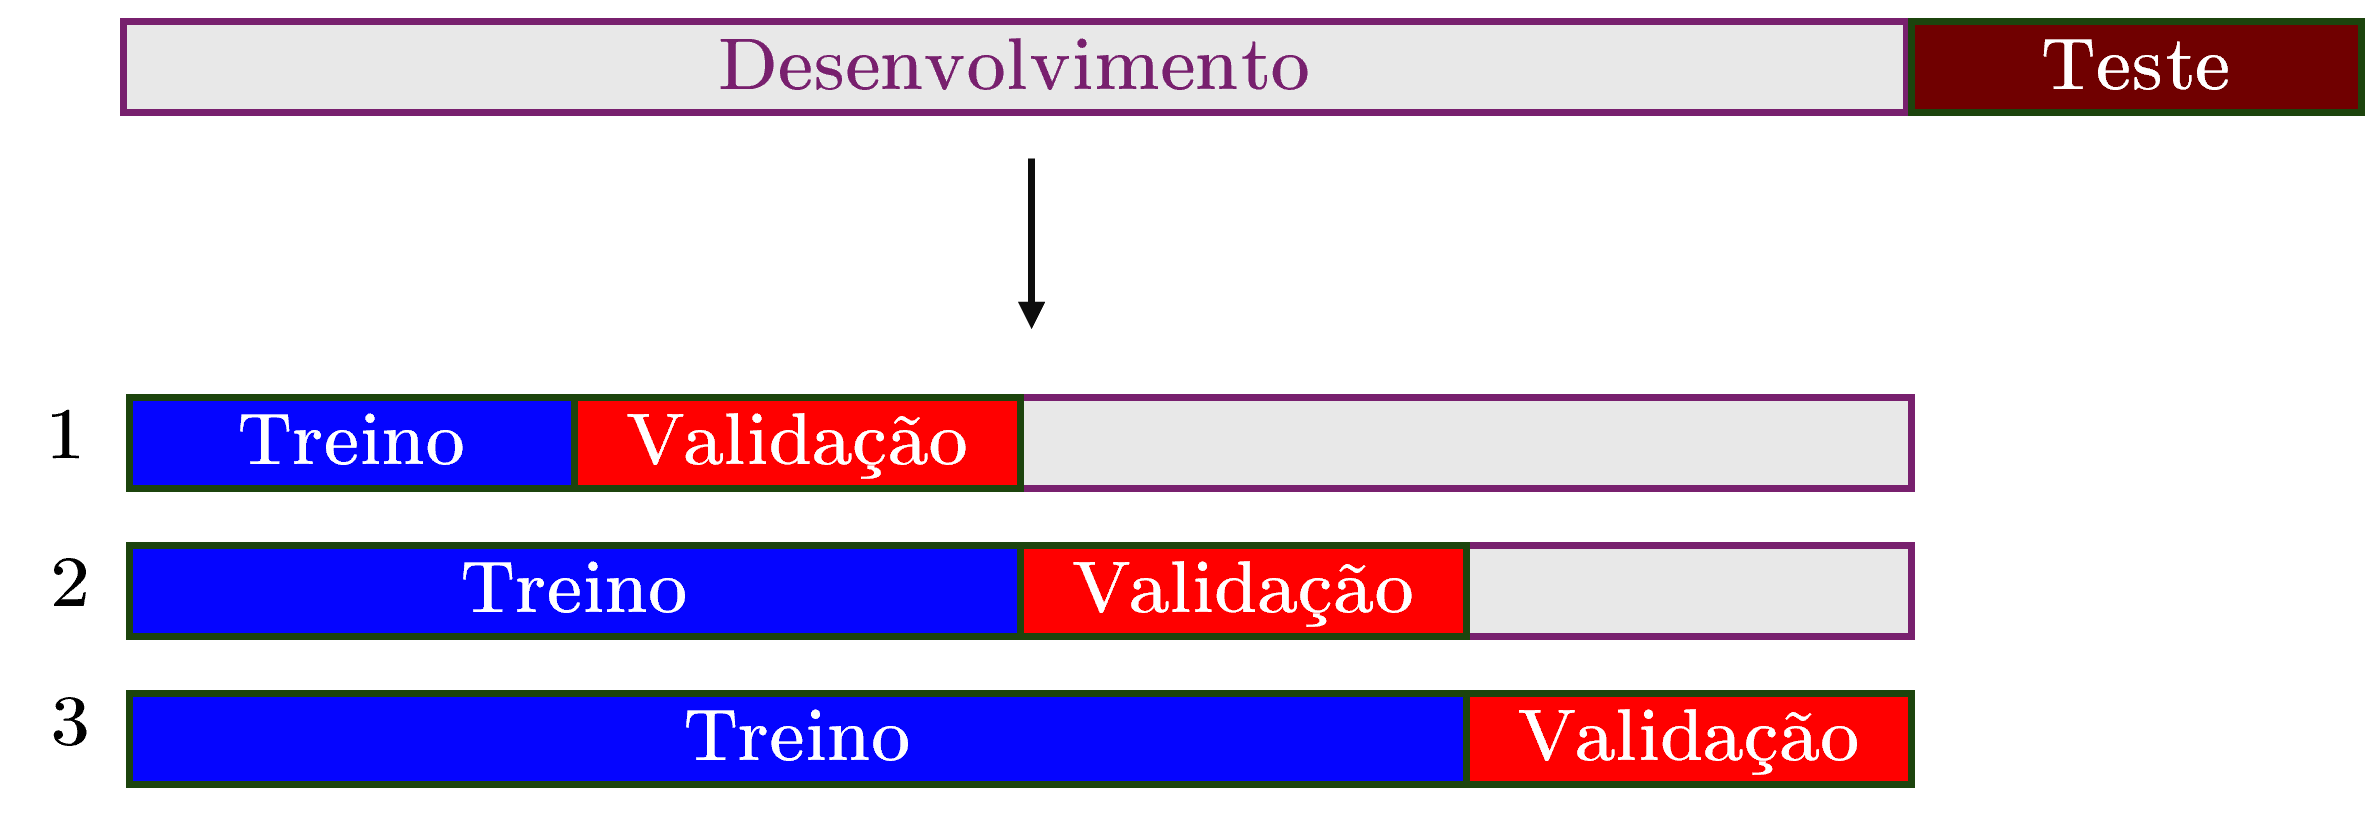
\includegraphics[width=\textwidth]{figuras/validacao_cruzada_teo.png}
			\caption{Validação Cruzada com 3 dobras}
			\label{fig:validacao_cruzada_teo}
		\end{center}
		\text{Fonte: Elaborado pelo autor, baseado em \cite{hyndman2018forecasting}}

	\end{center}
\end{figure}

\paragraph{} Após a subdivisão, os modelos serão treinados usando o conjunto de treinamento e seu desempenho será avaliado pelas medidas de desempenho: \ac{MAPE}, \ac{SLE}, \ac{MSE}, \ac{RMSE}, \(U_1\) e \(U_2\) de cada conjunto de validação e com os resultados serão calculados média e desvio padrão para cada medida. O melhor conjunto de hiperparâmetros será escolhido pelo algoritmo Optuna \cite{optuna_2019} e o ajuste fino será feito pela GridSearch.

\paragraph{} Após a definição dos hiperparâmetros com base nas medidas de desempenho, o modelo será treinado usando todo o conjunto de desenvolvimento e, em seguida, avaliado no conjunto de teste. Isso permitirá verificar sua capacidade de generalização para dados que não foram vistos anteriormente.

% ---------------------------------------------------------------
% Chapter N-1 - Resultados
% ---------------------------------------------------------------
\chapter{Resultados}
\label{resultados}
\paragraph{} Neste capítulo serão apresentados os resultados do modelo, avaliado pelas medidas de desempenho descritas anteriormente, junto com os gráficos da previsão do conjunto de teste.

\paragraph{} Os resultados serão apresentados para cada modelo, com os dois conjuntos de dados disponíveis: Biodiesel Nacional e Óleo de Soja e as duas abordagens de pré-processamento: remoção de tendência linear e normalização min-max. Os diferentes tipos de janelamento: Janela deslizante e Janela de Takens serão considerados modelos distintos.

\section{Janela Deslizante}

\paragraph{} Os resultados obtidos pelo modelo utilizando a abordagem de janela deslizante são apresentados nas Tabelas \ref{tab:resultados_validacao} e \ref{tab:resultados_teste}, que detalham as métricas de desempenho para cada cenário avaliado, tanto na validação cruzada quanto no conjunto de teste. Além disso, as Figuras \ref{fig:brasil_results}, \ref{fig:brasil_oil_results}, \ref{fig:brasil_results_test} e \ref{fig:brasil_oil_results_test} ilustram essa comparação de forma gráfica, representando os mesmos dados das tabelas em gráficos de pontos.
\paragraph{} As subseções a seguir discutem os resultados de cada modelo, abordando os gráficos de previsão e a distribuição dos resíduos. Serão apresentadas as previsões comparadas aos valores reais, além da análise da distribuição dos resíduos por meio de histogramas e gráficos de dispersão, com o objetivo de compreender o comportamento do modelo e avaliar sua adequação aos dados.

\subsection{\acs{NARX}}
\paragraph{} Conforme apresentado na Figura \ref{fig:narx_results} destaca-se que o modelo (b) foi o único capaz de mapear os dados reais de forma satisfatória, apresentando baixos valores de erro no conjunto de teste e mantendo essa performance de forma consistente no conjunto de desenvolvimento. Os resultados obtidos indicam que o desvio padrão dos erros foi inferior a 10\% das respectivas medidas, como detalhado nas Tabelas \ref{tab:resultados_validacao} e \ref{tab:resultados_teste}. Apesar do desempenho insatisfatório dos modelos (c) e (d), observa-se que ambos mantiveram consistência ao longo das validações.
\paragraph{} Além disso, ao analisar os gráficos de dispersão apresentados na Figura \ref{fig:narx_scatter}, observou-se que o modelo (b) exibe uma dispersão reduzida, evidenciando uma correlação positiva clara entre os valores previstos e observados. Em contraste, os modelos (a) e (c) demonstram maior dispersão para valores menores e uma redução dessa dispersão à medida que os valores aumentam, com uma linha de tendência também positiva. O modelo (d), por sua vez, apresenta uma dispersão considerável ao longo de todo o intervalo de valores, sem uma clara tendência.
\paragraph{} Por fim, os histogramas dos resíduos, ilustrados na Figura \ref{fig:narx_residuals_histogram}, revelam que o modelo (b) gera uma distribuição dos resíduos mais próxima de uma distribuição normal, embora com alguns valores discrepantes próximos a 0,2 e 0,3, que deslocam a média para a direita. Em contrapartida, os modelos (a), (c) e (d) exibem distribuições assimétricas, com a presença de valores discrepantes mais pronunciados, indicando um comportamento menos ideal na previsão dos resíduos.

\begin{figure}[htbp]
	\centering
	\begin{subfigure}[b]{0.45\textwidth}
		\centering
		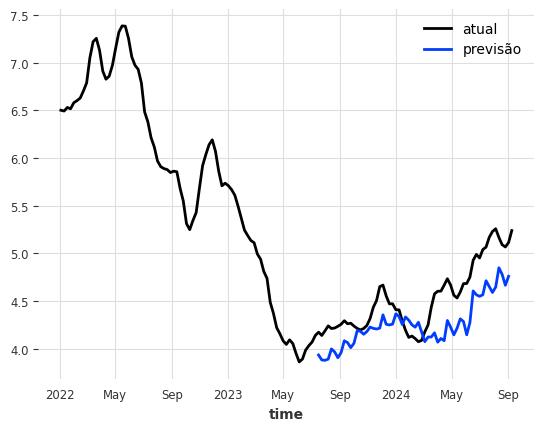
\includegraphics[width=\textwidth]{figuras/narx_brasil_plot.png} % Substitua pelo caminho da sua imagem
		\caption{Treinado com Biodiesel Nacional \newline}
		\label{fig:narx_brasil_plot}
	\end{subfigure}
	\hfill
	\begin{subfigure}[b]{0.45\textwidth}
		\centering
		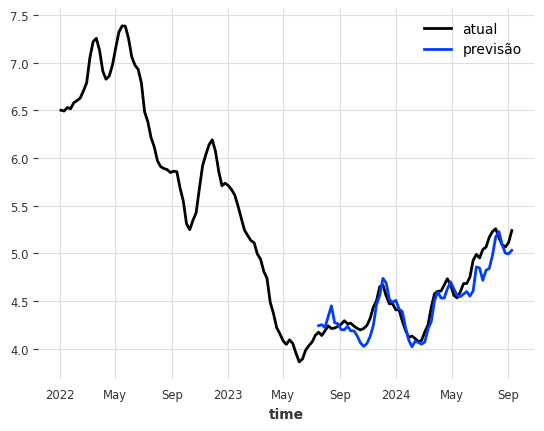
\includegraphics[width=\textwidth]{figuras/narx_brasil_oil_plot.png} % Substitua pelo caminho da sua imagem
		\caption{Treinado com Biodiesel Nacional e Óleo de Soja}
		\label{fig:narx_brasil_oil_plot}
	\end{subfigure}

	\vskip\baselineskip % Espaçamento vertical entre as linhas de imagens

	\begin{subfigure}[b]{0.45\textwidth}
		\centering
		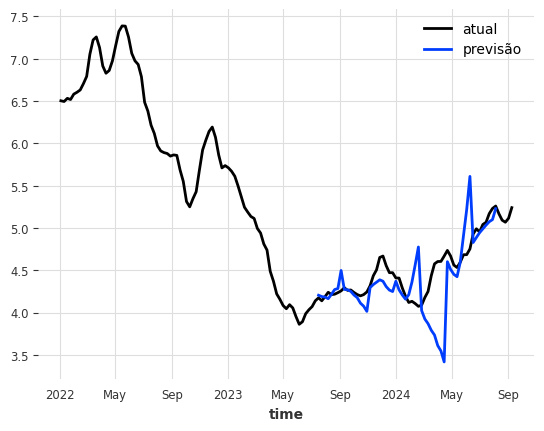
\includegraphics[width=\textwidth]{figuras/narx_brasil_detrend_plot.png} % Substitua pelo caminho da sua imagem
		\caption{Treinado com Biodiesel Nacional sem tendência}
		\label{fig:narx_brasil_detrend_plot}
	\end{subfigure}
	\hfill
	\begin{subfigure}[b]{0.45\textwidth}
		\centering
		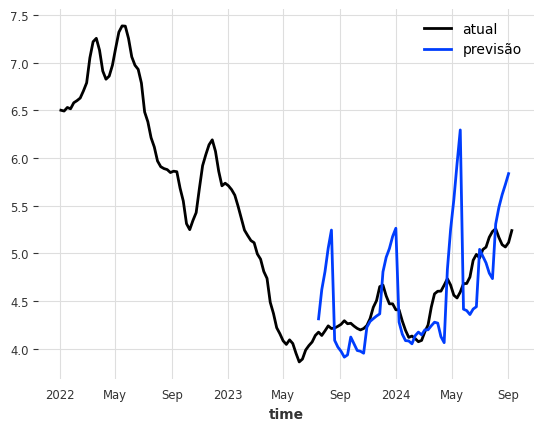
\includegraphics[width=\textwidth]{figuras/narx_brasil_oil_detrend_plot.png} % Substitua pelo caminho da sua imagem
		\caption{Treinado com Biodiesel Nacional e Óleo de Soja sem tendência}
		\label{fig:narx_brasil_oil_detrend_plot}
	\end{subfigure}

	\caption{Resultados do modelo \acs{NARX} no conjunto de teste}
	\label{fig:narx_results}
\end{figure}
\begin{figure}[htbp]
	\centering
	\begin{subfigure}[b]{0.40\textwidth}
		\centering
		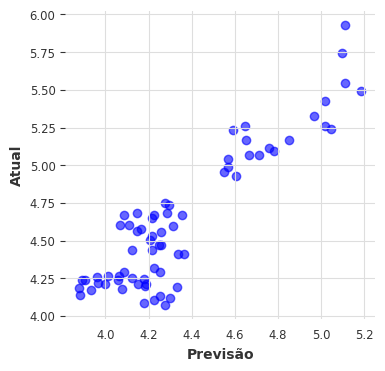
\includegraphics[width=\textwidth]{figuras/narx_brasil_scatter.png} % Substitua pelo caminho da sua imagem
		\caption{Treinado com Biodiesel Nacional \newline}
		\label{fig:narx_brasil_scatter}
	\end{subfigure}
	\hfill
	\begin{subfigure}[b]{0.40\textwidth}
		\centering
		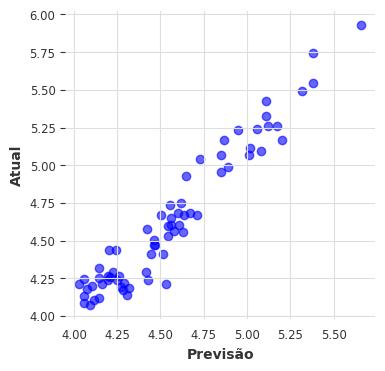
\includegraphics[width=\textwidth]{figuras/narx_brasil_oil_scatter.png} % Substitua pelo caminho da sua imagem
		\caption{Treinado com Biodiesel Nacional e Óleo de Soja}
		\label{fig:narx_brasil_oil_scatter}
	\end{subfigure}

	\vskip\baselineskip % Espaçamento vertical entre as linhas de imagens

	\begin{subfigure}[b]{0.40\textwidth}
		\centering
		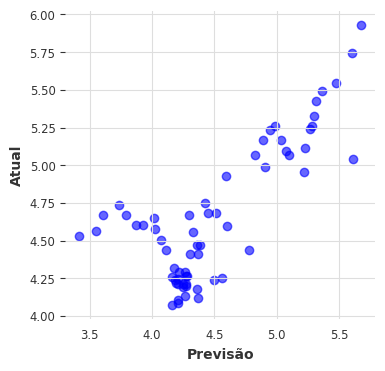
\includegraphics[width=\textwidth]{figuras/narx_brasil_detrend_scatter.png} % Substitua pelo caminho da sua imagem
		\caption{Treinado com Biodiesel Nacional sem tendência}
		\label{fig:narx_brasil_detrend_scatter}
	\end{subfigure}
	\hfill
	\begin{subfigure}[b]{0.40\textwidth}
		\centering
		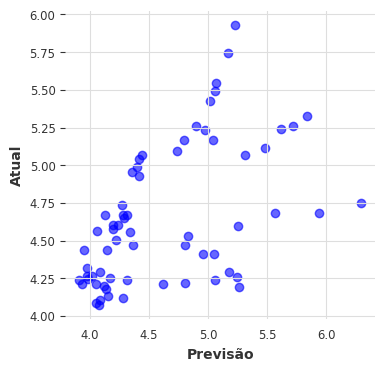
\includegraphics[width=\textwidth]{figuras/narx_brasil_oil_detrend_scatter.png} % Substitua pelo caminho da sua imagem
		\caption{Treinado com Biodiesel Nacional e Óleo de Soja sem tendência}
		\label{fig:narx_brasil_oil_detrend_scatter}
	\end{subfigure}

	\caption{Gráficos de dispersão dos valores atuais versus valores previstos pelo modelo \acs{NARX} no conjunto de teste}
	\label{fig:narx_scatter}
\end{figure}
\begin{figure}[htbp]
	\centering
	\begin{subfigure}[b]{0.40\textwidth}
		\centering
		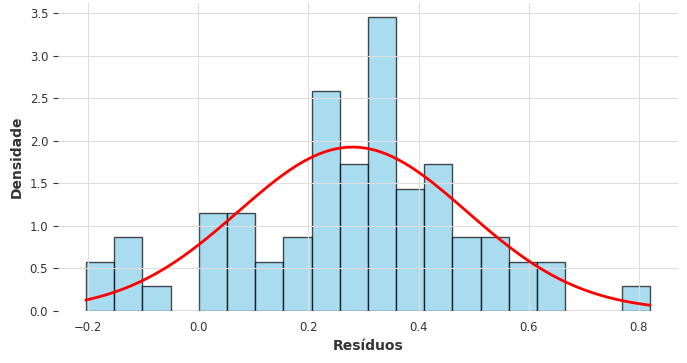
\includegraphics[width=\textwidth]{figuras/narx_brasil_residuals_histogram.png} % Substitua pelo caminho da sua imagem
		\caption{Treinado com Biodiesel Nacional \newline}
		\label{fig:narx_brasil_residuals_histogram}
	\end{subfigure}
	\hfill
	\begin{subfigure}[b]{0.40\textwidth}
		\centering
		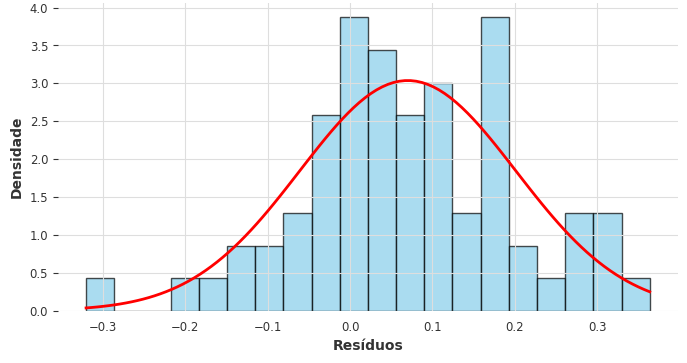
\includegraphics[width=\textwidth]{figuras/narx_brasil_oil_residuals_histogram.png} % Substitua pelo caminho da sua imagem
		\caption{Treinado com Biodiesel Nacional e Óleo de Soja}
		\label{fig:narx_brasil_oil_residuals_histogram}
	\end{subfigure}

	\vskip\baselineskip % Espaçamento vertical entre as linhas de imagens

	\begin{subfigure}[b]{0.40\textwidth}
		\centering
		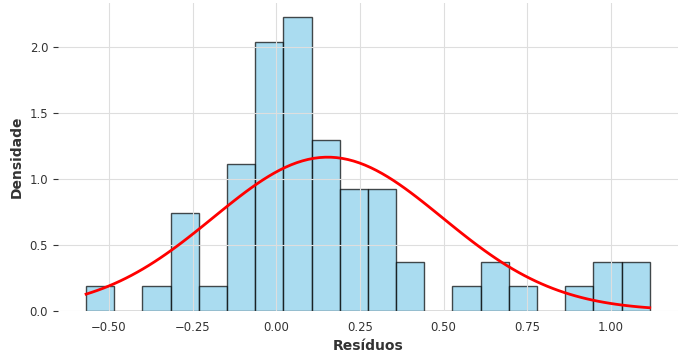
\includegraphics[width=\textwidth]{figuras/narx_brasil_detrend_residuals_histogram.png} % Substitua pelo caminho da sua imagem
		\caption{Treinado com Biodiesel Nacional sem tendência}
		\label{fig:narx_brasil_detrend_residuals_histogram}
	\end{subfigure}
	\hfill
	\begin{subfigure}[b]{0.40\textwidth}
		\centering
		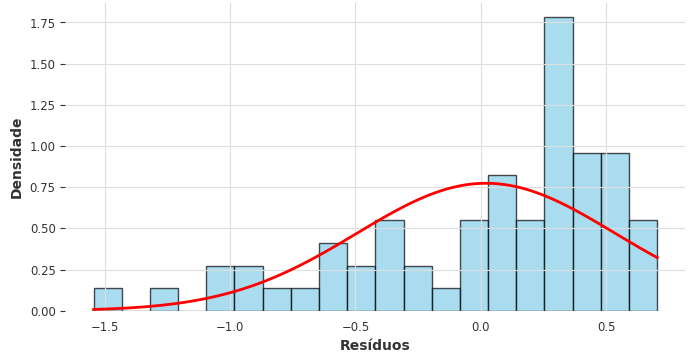
\includegraphics[width=\textwidth]{figuras/narx_brasil_oil_detrend_residuals_histogram.png} % Substitua pelo caminho da sua imagem
		\caption{Treinado com Biodiesel Nacional e Óleo de Soja sem tendência}
		\label{fig:narx_brasil_oil_detrend_residuals_histogram}
	\end{subfigure}

	\caption{Histograma dos erros do modelo \acs{NARX} no conjunto de teste}
	\label{fig:narx_residuals_histogram}
\end{figure}

\subsection{\acs{DA-RNN}}
\paragraph{} Como ilustrado na Figura \ref{fig:darnn_results}, o modelo (c) apresentou uma capacidade eficaz de mapeamento, reproduzindo de forma precisa os dados reais e alcançando baixos valores de erro no conjunto de teste, conforme exposto na Tabela \ref{tab:resultados_teste}. Contudo, os resultados obtidos no conjunto de desenvolvimento revelaram-se inconsistentes, sugerindo um possível superdimensionamento do modelo para este conjunto de dados, conforme indicado pela Tabela \ref{tab:resultados_validacao}. Ao comparar os resultados das Tabelas \ref{tab:resultados_validacao} e \ref{tab:resultados_teste}, nota-se uma inversão no desempenho: enquanto o modelo (c) obteve o melhor resultado no conjunto de teste, apresentou o pior desempenho no conjunto de desenvolvimento, ao passo que o modelo (d) demonstrou o comportamento oposto, que novamente sugere um superdimensionamento do modelo.
\paragraph{} Adicionalmente, ao examinar os gráficos de dispersão apresentados na Figura \ref{fig:darnn_scatter}, observou-se que o modelo (c) apresenta uma dispersão reduzida, o que indica uma correlação positiva clara entre os valores previstos e observados. Em contraste, os modelos (a), (b) e (d) exibem uma maior dispersão para valores mais baixos, com uma diminuição dessa dispersão à medida que os valores aumentam, sendo que a linha de tendência, embora também positiva, possui uma inclinação ligeiramente inferior a 1, sugerindo um aumento do erro conforme os valores reais se elevam.
\paragraph{} Por último, conforme ilustrado na Figura \ref{fig:darnn_residuals_histogram}, os histogramas dos resíduos indicam que o modelo (c) gera uma distribuição dos resíduos que se aproxima de uma distribuição normal, com um leve desvio para a direita. Em contrapartida, os modelos (a), (b) e (d) apresentam distribuições com caudas pesadas, sugerindo maior variabilidade nos erros de previsão.
\begin{figure}[htbp]
	\centering
	\begin{subfigure}[b]{0.45\textwidth}
		\centering
		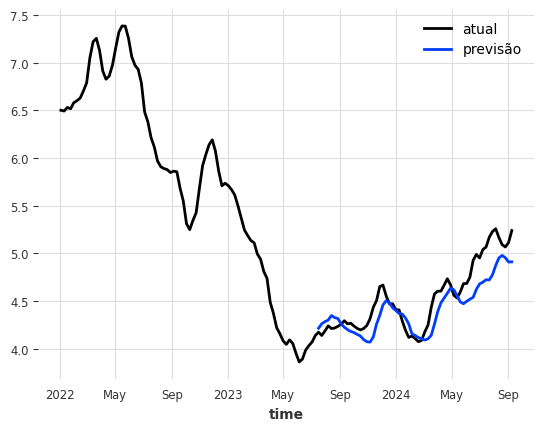
\includegraphics[width=\textwidth]{figuras/darnn_brasil_plot.png} % Substitua pelo caminho da sua imagem
		\caption{Treinado com Biodiesel Nacional \newline}
		\label{fig:darnn_brasil_plot}
	\end{subfigure}
	\hfill
	\begin{subfigure}[b]{0.45\textwidth}
		\centering
		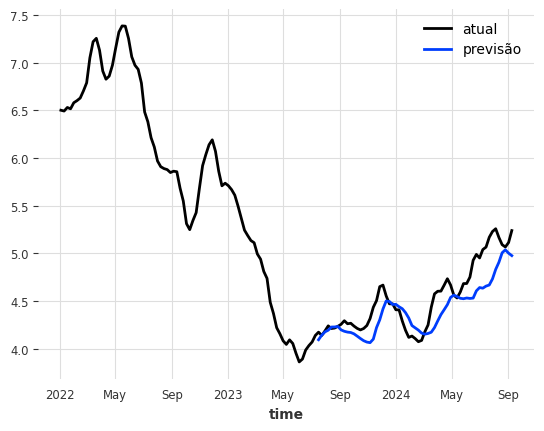
\includegraphics[width=\textwidth]{figuras/darnn_brasil_oil_plot.png} % Substitua pelo caminho da sua imagem
		\caption{Treinado com Biodiesel Nacional e Óleo de Soja}
		\label{fig:darnn_brasil_oil_plot}
	\end{subfigure}

	\vskip\baselineskip % Espaçamento vertical entre as linhas de imagens

	\begin{subfigure}[b]{0.45\textwidth}
		\centering
		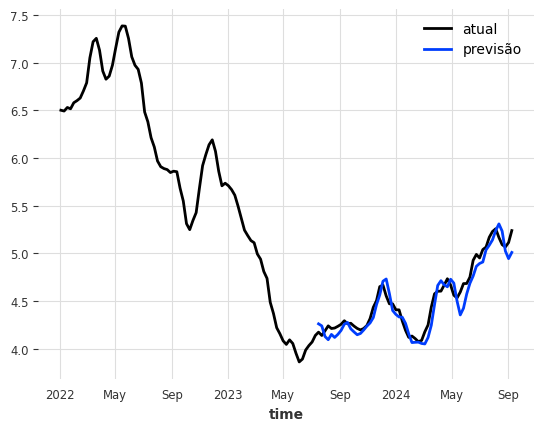
\includegraphics[width=\textwidth]{figuras/darnn_brasil_detrend_plot.png} % Substitua pelo caminho da sua imagem
		\caption{Treinado com Biodiesel Nacional sem tendência}
		\label{fig:darnn_brasil_detrend_plot}
	\end{subfigure}
	\hfill
	\begin{subfigure}[b]{0.45\textwidth}
		\centering
		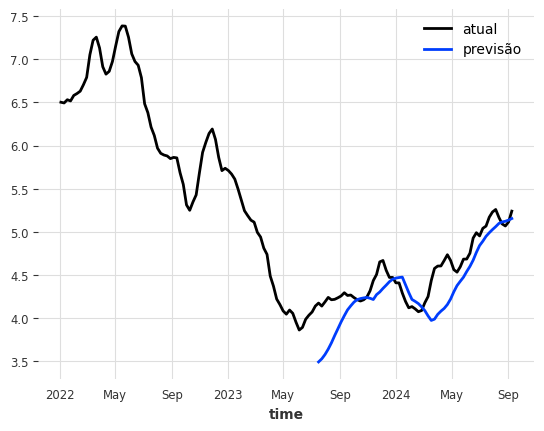
\includegraphics[width=\textwidth]{figuras/darnn_brasil_oil_detrend_plot.png} % Substitua pelo caminho da sua imagem
		\caption{Treinado com Biodiesel Nacional e Óleo de Soja sem tendência}
		\label{fig:darnn_brasil_oil_detrend_plot}
	\end{subfigure}

	\caption{Resultados do modelo \acs{DA-RNN} no conjunto de teste}
	\label{fig:darnn_results}
\end{figure}
\begin{figure}[htbp]
	\centering
	\begin{subfigure}[b]{0.40\textwidth}
		\centering
		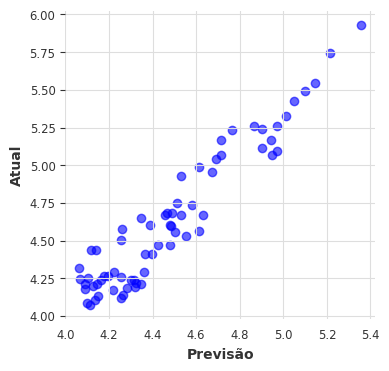
\includegraphics[width=\textwidth]{figuras/darnn_brasil_scatter.png} % Substitua pelo caminho da sua imagem
		\caption{Treinado com Biodiesel Nacional \newline}
		\label{fig:darnn_brasil_scatter}
	\end{subfigure}
	\hfill
	\begin{subfigure}[b]{0.40\textwidth}
		\centering
		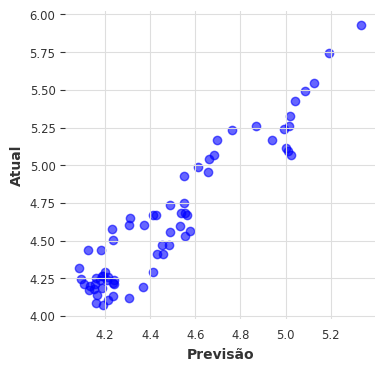
\includegraphics[width=\textwidth]{figuras/darnn_brasil_oil_scatter.png} % Substitua pelo caminho da sua imagem
		\caption{Treinado com Biodiesel Nacional e Óleo de Soja}
		\label{fig:darnn_brasil_oil_scatter}
	\end{subfigure}

	\vskip\baselineskip % Espaçamento vertical entre as linhas de imagens

	\begin{subfigure}[b]{0.40\textwidth}
		\centering
		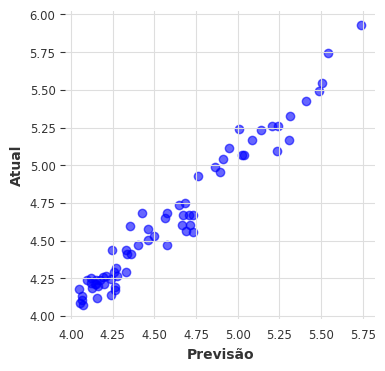
\includegraphics[width=\textwidth]{figuras/darnn_brasil_detrend_scatter.png} % Substitua pelo caminho da sua imagem
		\caption{Treinado com Biodiesel Nacional sem tendência}
		\label{fig:darnn_brasil_detrend_scatter}
	\end{subfigure}
	\hfill
	\begin{subfigure}[b]{0.40\textwidth}
		\centering
		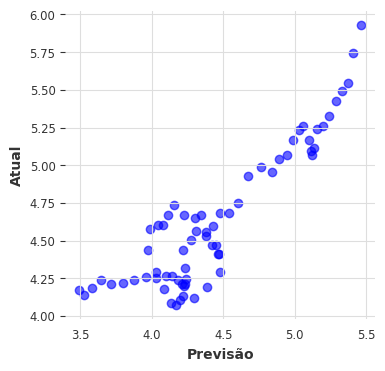
\includegraphics[width=\textwidth]{figuras/darnn_brasil_oil_detrend_scatter.png} % Substitua pelo caminho da sua imagem
		\caption{Treinado com Biodiesel Nacional e Óleo de Soja sem tendência}
		\label{fig:darnn_brasil_oil_detrend_scatter}
	\end{subfigure}

	\caption{Gráficos de dispersão dos valores atuais versus valores previstos pelo modelo \acs{DA-RNN} no conjunto de teste}
	\label{fig:darnn_scatter}
\end{figure}
\begin{figure}[htbp]
	\centering
	\begin{subfigure}[b]{0.40\textwidth}
		\centering
		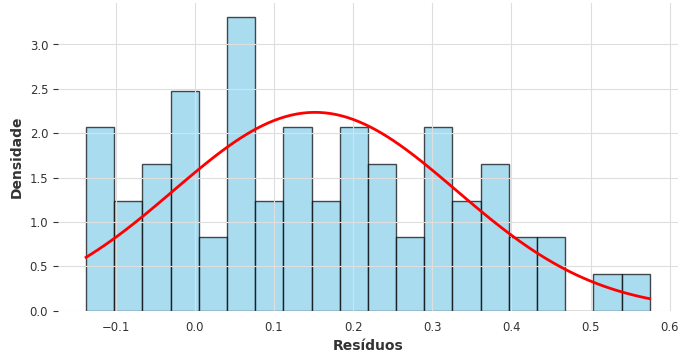
\includegraphics[width=\textwidth]{figuras/darnn_brasil_residuals_histogram.png} % Substitua pelo caminho da sua imagem
		\caption{Treinado com Biodiesel Nacional \newline}
		\label{fig:darnn_brasil_residuals_histogram}
	\end{subfigure}
	\hfill
	\begin{subfigure}[b]{0.40\textwidth}
		\centering
		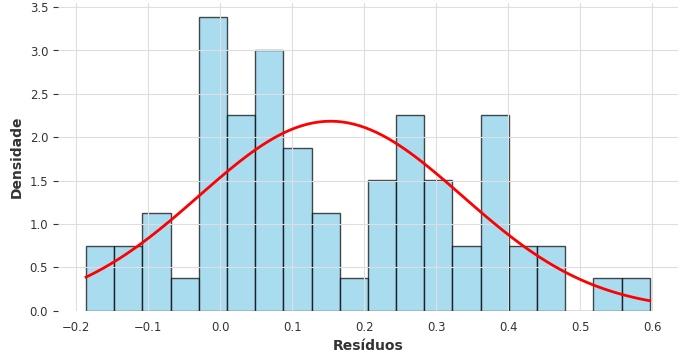
\includegraphics[width=\textwidth]{figuras/darnn_brasil_oil_residuals_histogram.png} % Substitua pelo caminho da sua imagem
		\caption{Treinado com Biodiesel Nacional e Óleo de Soja}
		\label{fig:darnn_brasil_oil_residuals_histogram}
	\end{subfigure}

	\vskip\baselineskip % Espaçamento vertical entre as linhas de imagens

	\begin{subfigure}[b]{0.40\textwidth}
		\centering
		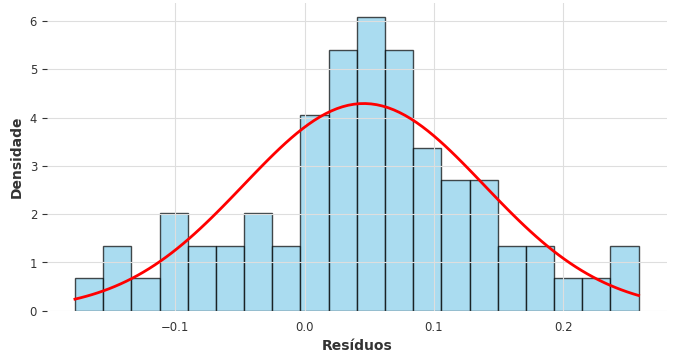
\includegraphics[width=\textwidth]{figuras/darnn_brasil_detrend_residuals_histogram.png} % Substitua pelo caminho da sua imagem
		\caption{Treinado com Biodiesel Nacional sem tendência}
		\label{fig:darnn_brasil_detrend_residuals_histogram}
	\end{subfigure}
	\hfill
	\begin{subfigure}[b]{0.40\textwidth}
		\centering
		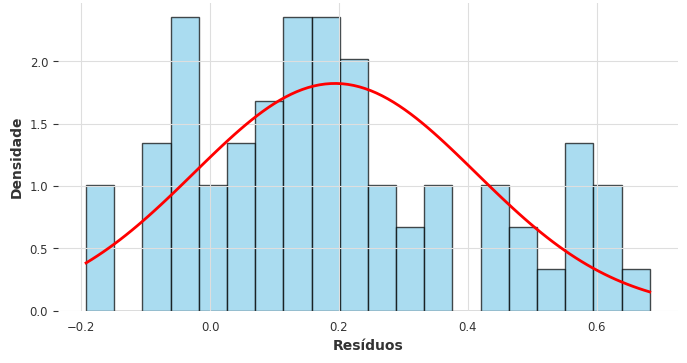
\includegraphics[width=\textwidth]{figuras/darnn_brasil_oil_detrend_residuals_histogram.png} % Substitua pelo caminho da sua imagem
		\caption{Treinado com Biodiesel Nacional e Óleo de Soja sem tendência}
		\label{fig:darnn_brasil_oil_detrend_residuals_histogram}
	\end{subfigure}

	\caption{Histograma dos erros do modelo \acs{DA-RNN} no conjunto de teste}
	\label{fig:darnn_residuals_histogram}
\end{figure}

\subsection{\acs{MLP}}
\paragraph{} Como mostrado na Tabela \ref{tab:resultados_teste} e na Figura \ref{fig:mlp_results}, os modelos (c) e (d) apresentaram os menores valores de erro entre todos os modelos baseados em janela deslizante. No entanto, apenas os modelos (b) e (d), que utilizaram um conjunto de treinamento mais extenso, mostraram resultados consistentes no conjunto de desenvolvimento, como evidenciado na Tabela \ref{tab:resultados_validacao}. Esse desempenho sugere que o tamanho do conjunto de treinamento desempenha um papel importante na capacidade de generalização do modelo.
\paragraph{} Adicionalmente, a análise dos gráficos de dispersão apresentados na Figura \ref{fig:mlp_scatter} revelou que os modelos (c) e (d) exibem uma dispersão reduzida, com correlação próxima de 1, indicando um bom ajuste entre os valores previstos e observados. Em contraste, os modelos (a) e (b) apresentaram maior dispersão, com as linhas de tendência mostrando uma inclinação ligeiramente superior a 1, sugerindo um aumento no erro conforme os valores reais aumentam.
\paragraph{} Por fim, ao examinar os histogramas dos resíduos, apresentados na Figura \ref{fig:mlp_residuals_histogram}, observou-se que os modelos (a), (b) e (d) exibem distribuições que se aproximam de uma distribuição normal, embora com a presença de múltiplos picos. Em contrapartida, o modelo (c) demonstrou uma distribuição assimétrica, com maior concentração de resíduos em torno de zero.

\begin{figure}[htbp]
	\centering
	\begin{subfigure}[b]{0.45\textwidth}
		\centering
		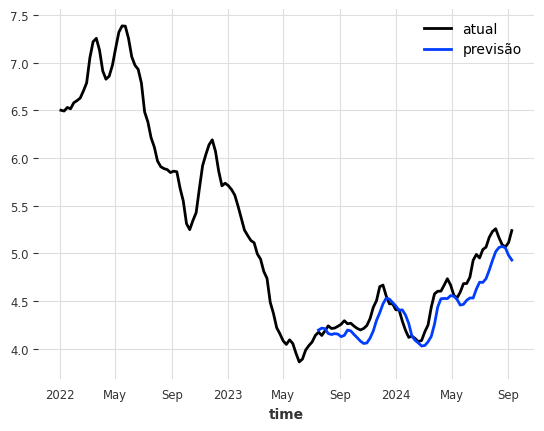
\includegraphics[width=\textwidth]{figuras/mlp_brasil_plot.png} % Substitua pelo caminho da sua imagem
		\caption{Treinado com Biodiesel Nacional \newline}
		\label{fig:mlp_brasil_plot}
	\end{subfigure}
	\hfill
	\begin{subfigure}[b]{0.45\textwidth}
		\centering
		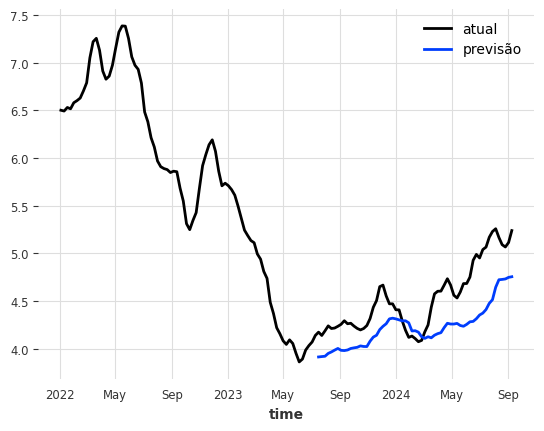
\includegraphics[width=\textwidth]{figuras/mlp_brasil_oil_plot.png} % Substitua pelo caminho da sua imagem
		\caption{Treinado com Biodiesel Nacional e Óleo de Soja}
		\label{fig:mlp_brasil_oil_plot}
	\end{subfigure}

	\vskip\baselineskip % Espaçamento vertical entre as linhas de imagens

	\begin{subfigure}[b]{0.45\textwidth}
		\centering
		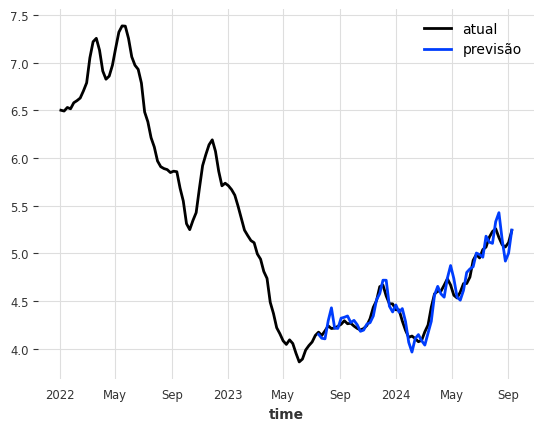
\includegraphics[width=\textwidth]{figuras/mlp_brasil_detrend_plot.png} % Substitua pelo caminho da sua imagem
		\caption{Treinado com Biodiesel Nacional sem tendência}
		\label{fig:mlp_brasil_detrend_plot}
	\end{subfigure}
	\hfill
	\begin{subfigure}[b]{0.45\textwidth}
		\centering
		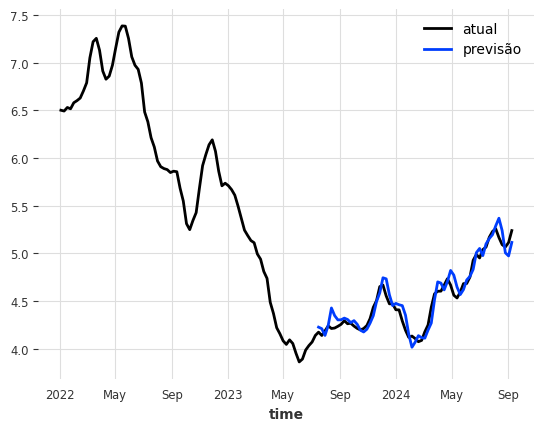
\includegraphics[width=\textwidth]{figuras/mlp_brasil_oil_detrend_plot.png} % Substitua pelo caminho da sua imagem
		\caption{Treinado com Biodiesel Nacional e Óleo de Soja sem tendência}
		\label{fig:mlp_brasil_oil_detrend_plot}
	\end{subfigure}

	\caption{Resultados do modelo \acs{MLP} no conjunto de teste}
	\label{fig:mlp_results}
\end{figure}
\begin{figure}[htbp]
	\centering
	\begin{subfigure}[b]{0.40\textwidth}
		\centering
		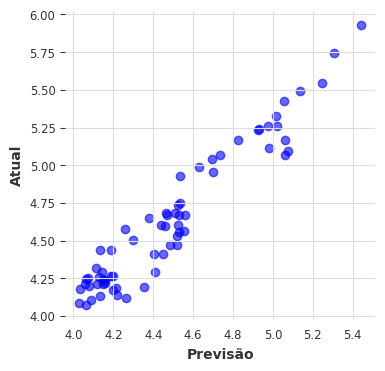
\includegraphics[width=\textwidth]{figuras/mlp_brasil_scatter.png} % Substitua pelo caminho da sua imagem
		\caption{Treinado com Biodiesel Nacional \newline}
		\label{fig:mlp_brasil_scatter}
	\end{subfigure}
	\hfill
	\begin{subfigure}[b]{0.40\textwidth}
		\centering
		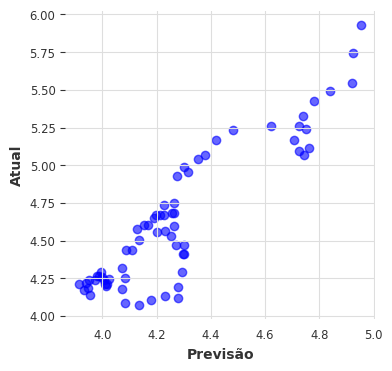
\includegraphics[width=\textwidth]{figuras/mlp_brasil_oil_scatter.png} % Substitua pelo caminho da sua imagem
		\caption{Treinado com Biodiesel Nacional e Óleo de Soja}
		\label{fig:mlp_brasil_oil_scatter}
	\end{subfigure}

	\vskip\baselineskip % Espaçamento vertical entre as linhas de imagens

	\begin{subfigure}[b]{0.40\textwidth}
		\centering
		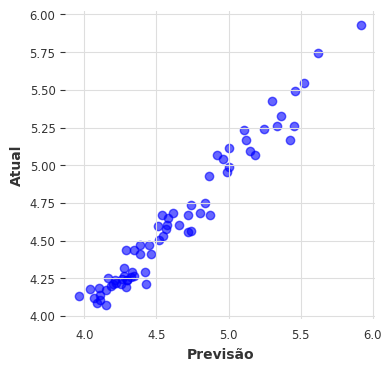
\includegraphics[width=\textwidth]{figuras/mlp_brasil_detrend_scatter.png} % Substitua pelo caminho da sua imagem
		\caption{Treinado com Biodiesel Nacional sem tendência}
		\label{fig:mlp_brasil_detrend_scatter}
	\end{subfigure}
	\hfill
	\begin{subfigure}[b]{0.40\textwidth}
		\centering
		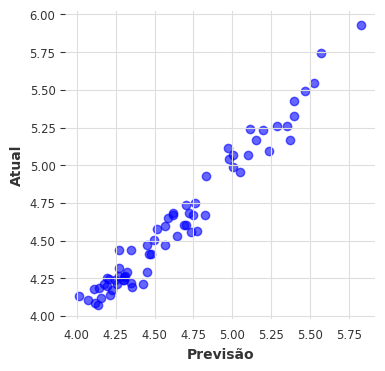
\includegraphics[width=\textwidth]{figuras/mlp_brasil_oil_detrend_scatter.png} % Substitua pelo caminho da sua imagem
		\caption{Treinado com Biodiesel Nacional e Óleo de Soja sem tendência}
		\label{fig:mlp_brasil_oil_detrend_scatter}
	\end{subfigure}

	\caption{Gráficos de dispersão dos valores atuais versus valores previstos pelo modelo \acs{MLP} no conjunto de teste}
	\label{fig:mlp_scatter}
\end{figure}
\begin{figure}[htbp]
	\centering
	\begin{subfigure}[b]{0.40\textwidth}
		\centering
		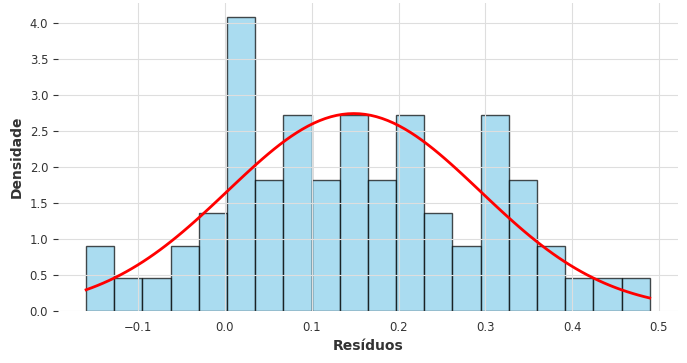
\includegraphics[width=\textwidth]{figuras/mlp_brasil_residuals_histogram.png} % Substitua pelo caminho da sua imagem
		\caption{Treinado com Biodiesel Nacional \newline}
		\label{fig:mlp_brasil_residuals_histogram}
	\end{subfigure}
	\hfill
	\begin{subfigure}[b]{0.40\textwidth}
		\centering
		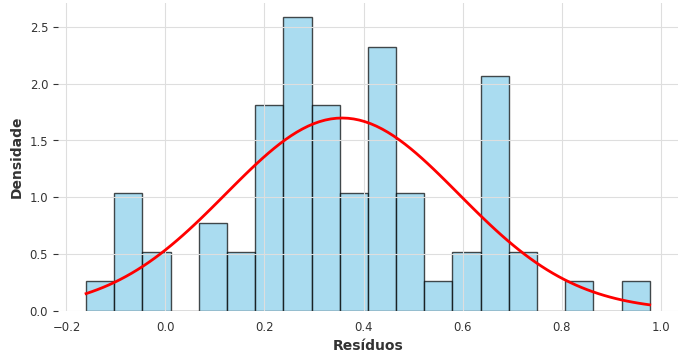
\includegraphics[width=\textwidth]{figuras/mlp_brasil_oil_residuals_histogram.png} % Substitua pelo caminho da sua imagem
		\caption{Treinado com Biodiesel Nacional e Óleo de Soja}
		\label{fig:mlp_brasil_oil_residuals_histogram}
	\end{subfigure}

	\vskip\baselineskip % Espaçamento vertical entre as linhas de imagens

	\begin{subfigure}[b]{0.40\textwidth}
		\centering
		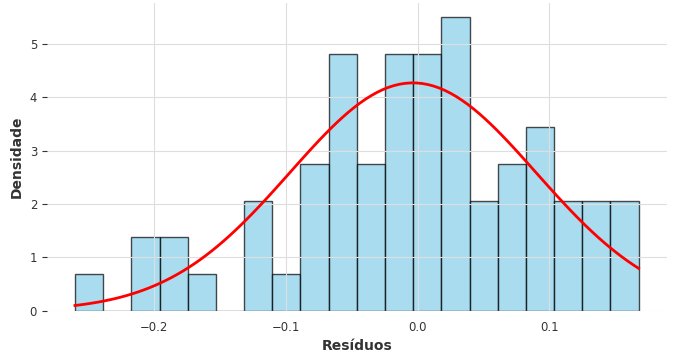
\includegraphics[width=\textwidth]{figuras/mlp_brasil_detrend_residuals_histogram.png} % Substitua pelo caminho da sua imagem
		\caption{Treinado com Biodiesel Nacional sem tendência}
		\label{fig:mlp_brasil_detrend_residuals_histogram}
	\end{subfigure}
	\hfill
	\begin{subfigure}[b]{0.40\textwidth}
		\centering
		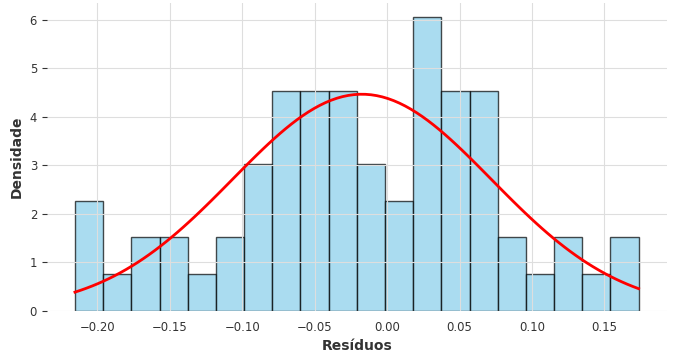
\includegraphics[width=\textwidth]{figuras/mlp_brasil_oil_detrend_residuals_histogram.png} % Substitua pelo caminho da sua imagem
		\caption{Treinado com Biodiesel Nacional e Óleo de Soja sem tendência}
		\label{fig:mlp_brasil_oil_detrend_residuals_histogram}
	\end{subfigure}

	\caption{Histograma dos erros do modelo \acs{MLP} no conjunto de teste}
	\label{fig:mlp_residuals_histogram}
\end{figure}

\subsection{\acs{IMP}}
\paragraph{} O modelo \ac{IMP} apresentou resultados inconsistentes em todos os cenários analisados e não obteve um desempenho satisfatório no conjunto de teste, conforme ilustrado na Figura \ref{fig:imp_results}.
\paragraph{} Adicionalmente, ao examinar os gráficos de dispersão apresentados na Figura \ref{fig:imp_scatter}, observou-se uma alta dispersão nos valores previstos por todos os modelos, indicando uma correlação fraca entre os valores previstos e observados. Os histogramas dos resíduos, apresentados na Figura \ref{fig:imp_residuals_histogram}, revelaram distribuições assimétricas e bimodais, sugerindo uma variabilidade incomum nos erros de previsão.

\begin{figure}[htbp]
	\centering
	\begin{subfigure}[b]{0.45\textwidth}
		\centering
		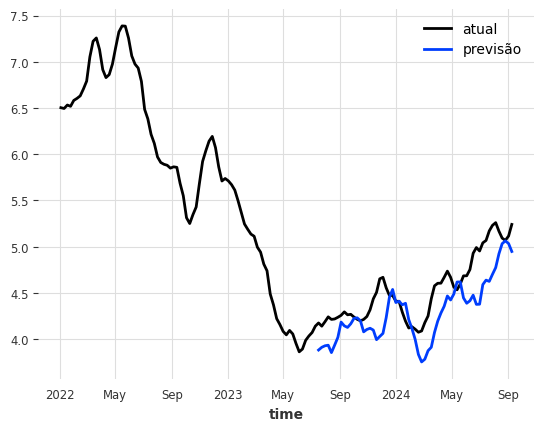
\includegraphics[width=\textwidth]{figuras/imp_brasil_plot.png} % Substitua pelo caminho da sua imagem
		\caption{Treinado com Biodiesel Nacional \newline}
		\label{fig:imp_brasil_plot}
	\end{subfigure}
	\hfill
	\begin{subfigure}[b]{0.45\textwidth}
		\centering
		\includegraphics[width=\textwidth]{figuras/imp_brasil_oil_plot.png} % Substitua pelo caminho da sua imagem
		\caption{Treinado com Biodiesel Nacional e Óleo de Soja}
		\label{fig:imp_brasil_oil_plot}
	\end{subfigure}

	\vskip\baselineskip % Espaçamento vertical entre as linhas de imagens

	\begin{subfigure}[b]{0.45\textwidth}
		\centering
		\includegraphics[width=\textwidth]{figuras/imp_brasil_detrend_plot.png} % Substitua pelo caminho da sua imagem
		\caption{Treinado com Biodiesel Nacional sem tendência}
		\label{fig:imp_brasil_detrend_plot}
	\end{subfigure}
	\hfill
	\begin{subfigure}[b]{0.45\textwidth}
		\centering
		\includegraphics[width=\textwidth]{figuras/imp_brasil_oil_detrend_plot.png} % Substitua pelo caminho da sua imagem
		\caption{Treinado com Biodiesel Nacional e Óleo de Soja sem tendência}
		\label{fig:imp_brasil_oil_detrend_plot}
	\end{subfigure}

	\caption{Resultados do modelo \acs{IMP} no conjunto de teste}
	\label{fig:imp_results}
\end{figure}
\begin{figure}[htbp]
	\centering
	\begin{subfigure}[b]{0.40\textwidth}
		\centering
		\includegraphics[width=\textwidth]{figuras/imp_brasil_scatter.png} % Substitua pelo caminho da sua imagem
		\caption{Treinado com Biodiesel Nacional \newline}
		\label{fig:imp_brasil_scatter}
	\end{subfigure}
	\hfill
	\begin{subfigure}[b]{0.40\textwidth}
		\centering
		\includegraphics[width=\textwidth]{figuras/imp_brasil_oil_scatter.png} % Substitua pelo caminho da sua imagem
		\caption{Treinado com Biodiesel Nacional e Óleo de Soja}
		\label{fig:imp_brasil_oil_scatter}
	\end{subfigure}

	\vskip\baselineskip % Espaçamento vertical entre as linhas de imagens

	\begin{subfigure}[b]{0.40\textwidth}
		\centering
		\includegraphics[width=\textwidth]{figuras/imp_brasil_detrend_scatter.png} % Substitua pelo caminho da sua imagem
		\caption{Treinado com Biodiesel Nacional sem tendência}
		\label{fig:imp_brasil_detrend_scatter}
	\end{subfigure}
	\hfill
	\begin{subfigure}[b]{0.40\textwidth}
		\centering
		\includegraphics[width=\textwidth]{figuras/imp_brasil_oil_detrend_scatter.png} % Substitua pelo caminho da sua imagem
		\caption{Treinado com Biodiesel Nacional e Óleo de Soja sem tendência}
		\label{fig:imp_brasil_oil_detrend_scatter}
	\end{subfigure}

	\caption{Gráficos de dispersão dos valores atuais versus valores previstos pelo modelo \acs{IMP} no conjunto de teste}
	\label{fig:imp_scatter}
\end{figure}
\begin{figure}[htbp]
	\centering
	\begin{subfigure}[b]{0.40\textwidth}
		\centering
		\includegraphics[width=\textwidth]{figuras/imp_brasil_residuals_histogram.png} % Substitua pelo caminho da sua imagem
		\caption{Treinado com Biodiesel Nacional \newline}
		\label{fig:imp_brasil_residuals_histogram}
	\end{subfigure}
	\hfill
	\begin{subfigure}[b]{0.40\textwidth}
		\centering
		\includegraphics[width=\textwidth]{figuras/imp_brasil_oil_residuals_histogram.png} % Substitua pelo caminho da sua imagem
		\caption{Treinado com Biodiesel Nacional e Óleo de Soja}
		\label{fig:imp_brasil_oil_residuals_histogram}
	\end{subfigure}

	\vskip\baselineskip % Espaçamento vertical entre as linhas de imagens

	\begin{subfigure}[b]{0.40\textwidth}
		\centering
		\includegraphics[width=\textwidth]{figuras/imp_brasil_detrend_residuals_histogram.png} % Substitua pelo caminho da sua imagem
		\caption{Treinado com Biodiesel Nacional sem tendência}
		\label{fig:imp_brasil_detrend_residuals_histogram}
	\end{subfigure}
	\hfill
	\begin{subfigure}[b]{0.40\textwidth}
		\centering
		\includegraphics[width=\textwidth]{figuras/imp_brasil_oil_detrend_residuals_histogram.png} % Substitua pelo caminho da sua imagem
		\caption{Treinado com Biodiesel Nacional e Óleo de Soja sem tendência}
		\label{fig:imp_brasil_oil_detrend_residuals_histogram}
	\end{subfigure}

	\caption{Histograma dos erros do modelo \acs{IMP} no conjunto de teste}
	\label{fig:imp_residuals_histogram}
\end{figure}

\subsection{\acs{IDLN}}
\paragraph{} Conforme mostrado na Figura \ref{fig:idln_results}, os modelos (a) e (c) apresentaram bons resultados no conjunto de teste, embora tenham demonstrado inconsistência no conjunto de desenvolvimento, como evidenciado na Tabela \ref{tab:resultados_teste}. Essa discrepância pode indicar que, apesar de seu bom desempenho em condições controladas, esses modelos enfrentam dificuldades em generalizar adequadamente para dados não vistos durante o treinamento.
\paragraph{} Além disso, ao analisar os gráficos de dispersão apresentados na Figura \ref{fig:idln_scatter}, observou-se que os modelos (a) e (c) exibem uma dispersão reduzida, com uma correlação positiva clara entre os valores previstos e observados, embora o modelo (a) apresente uma correlação superior a 1. Em contraste, os modelos (b) e (d) apresentam uma dispersão maior, com uma correlação aparentemente não linear. O modelo (b), em particular, demonstrou uma alta dispersão.
\paragraph{} Por fim, ao examinar os histogramas apresentados na Figura \ref{fig:idln_residuals_histogram}, observou-se que o modelo (c) apresenta uma distribuição dos resíduos próxima a uma distribuição normal, enquanto os demais modelos exibem distribuições irregulares, com caudas pesadas e múltiplas modas.

\begin{figure}[htbp]
	\centering
	\begin{subfigure}[b]{0.45\textwidth}
		\centering
		\includegraphics[width=\textwidth]{figuras/idln_brasil_plot.png} % Substitua pelo caminho da sua imagem
		\caption{Treinado com Biodiesel Nacional \newline}
		\label{fig:idln_brasil_plot}
	\end{subfigure}
	\hfill
	\begin{subfigure}[b]{0.45\textwidth}
		\centering
		\includegraphics[width=\textwidth]{figuras/idln_brasil_oil_plot.png} % Substitua pelo caminho da sua imagem
		\caption{Treinado com Biodiesel Nacional e Óleo de Soja}
		\label{fig:idln_brasil_oil_plot}
	\end{subfigure}

	\vskip\baselineskip % Espaçamento vertical entre as linhas de imagens

	\begin{subfigure}[b]{0.45\textwidth}
		\centering
		\includegraphics[width=\textwidth]{figuras/idln_brasil_detrend_plot.png} % Substitua pelo caminho da sua imagem
		\caption{Treinado com Biodiesel Nacional sem tendência}
		\label{fig:idln_brasil_detrend_plot}
	\end{subfigure}
	\hfill
	\begin{subfigure}[b]{0.45\textwidth}
		\centering
		\includegraphics[width=\textwidth]{figuras/idln_brasil_oil_detrend_plot.png} % Substitua pelo caminho da sua imagem
		\caption{Treinado com Biodiesel Nacional e Óleo de Soja sem tendência}
		\label{fig:idln_brasil_oil_detrend_plot}
	\end{subfigure}
	\caption{Resultados do modelo \acs{IDLN} no conjunto de teste}

	\label{fig:idln_results}
\end{figure}
\begin{figure}[htbp]
	\centering
	\begin{subfigure}[b]{0.40\textwidth}
		\centering
		\includegraphics[width=\textwidth]{figuras/idln_brasil_scatter.png} % Substitua pelo caminho da sua imagem
		\caption{Treinado com Biodiesel Nacional \newline}
		\label{fig:idln_brasil_scatter}
	\end{subfigure}
	\hfill
	\begin{subfigure}[b]{0.40\textwidth}
		\centering
		\includegraphics[width=\textwidth]{figuras/idln_brasil_oil_scatter.png} % Substitua pelo caminho da sua imagem
		\caption{Treinado com Biodiesel Nacional e Óleo de Soja}
		\label{fig:idln_brasil_oil_scatter}
	\end{subfigure}

	\vskip\baselineskip % Espaçamento vertical entre as linhas de imagens

	\begin{subfigure}[b]{0.40\textwidth}
		\centering
		\includegraphics[width=\textwidth]{figuras/idln_brasil_detrend_scatter.png} % Substitua pelo caminho da sua imagem
		\caption{Treinado com Biodiesel Nacional sem tendência}
		\label{fig:idln_brasil_detrend_scatter}
	\end{subfigure}
	\hfill
	\begin{subfigure}[b]{0.40\textwidth}
		\centering
		\includegraphics[width=\textwidth]{figuras/idln_brasil_oil_detrend_scatter.png} % Substitua pelo caminho da sua imagem
		\caption{Treinado com Biodiesel Nacional e Óleo de Soja sem tendência}
		\label{fig:idln_brasil_oil_detrend_scatter}
	\end{subfigure}

	\caption{Gráficos de dispersão dos valores atuais versus valores previstos pelo modelo \acs{IDLN} no conjunto de teste}
	\label{fig:idln_scatter}
\end{figure}
\begin{figure}[htbp]
	\centering
	\begin{subfigure}[b]{0.40\textwidth}
		\centering
		\includegraphics[width=\textwidth]{figuras/idln_brasil_residuals_histogram.png} % Substitua pelo caminho da sua imagem
		\caption{Treinado com Biodiesel Nacional \newline}
		\label{fig:idln_brasil_residuals_histogram}
	\end{subfigure}
	\hfill
	\begin{subfigure}[b]{0.40\textwidth}
		\centering
		\includegraphics[width=\textwidth]{figuras/idln_brasil_oil_residuals_histogram.png} % Substitua pelo caminho da sua imagem
		\caption{Treinado com Biodiesel Nacional e Óleo de Soja}
		\label{fig:idln_brasil_oil_residuals_histogram}
	\end{subfigure}

	\vskip\baselineskip % Espaçamento vertical entre as linhas de imagens

	\begin{subfigure}[b]{0.40\textwidth}
		\centering
		\includegraphics[width=\textwidth]{figuras/idln_brasil_detrend_residuals_histogram.png} % Substitua pelo caminho da sua imagem
		\caption{Treinado com Biodiesel Nacional sem tendência}
		\label{fig:idln_brasil_detrend_residuals_histogram}
	\end{subfigure}
	\hfill
	\begin{subfigure}[b]{0.40\textwidth}
		\centering
		\includegraphics[width=\textwidth]{figuras/idln_brasil_oil_detrend_residuals_histogram.png} % Substitua pelo caminho da sua imagem
		\caption{Treinado com Biodiesel Nacional e Óleo de Soja sem tendência}
		\label{fig:idln_brasil_oil_detrend_residuals_histogram}
	\end{subfigure}

	\caption{Histograma dos erros do modelo \acs{IDLN} no conjunto de teste}
	\label{fig:idln_residuals_histogram}
\end{figure}

\subsection{\acs{N-Linear}}
\paragraph{} Conforme mostrado na Figura \ref{fig:nlinear_results}, os modelos (a) e (c) alcançaram um mapeamento próximo aos valores reais, destacando-se como os melhores no conjunto de teste. No entanto, de acordo com a Tabela \ref{tab:resultados_validacao}, esses resultados mostraram-se inconsistentes ao longo dos diferentes conjuntos de validação cruzada, sugerindo uma possível falta de robustez na generalização dos modelos para diferentes subconjuntos de dados.
\paragraph{} Além disso, a análise dos gráficos de dispersão apresentados na Figura \ref{fig:nlinear_scatter} revela que os modelos (a) e (c) apresentam baixa dispersão e uma clara correlação entre as previsões e os dados reais. Por outro lado, os modelos (b) e (d) exibem maior dispersão, embora ainda seja possível observar uma correlação positiva entre os valores previstos e observados.
\paragraph{} Por fim, ao examinar os histogramas apresentados na Figura \ref{fig:nlinear_residuals_histogram}, observou-se que o modelo (b) se aproxima de uma distribuição normal, enquanto os demais modelos apresentam um comportamento multimodal, com várias modas nas distribuições dos resíduos.

\begin{figure}[htbp]
	\centering
	\begin{subfigure}[b]{0.45\textwidth}
		\centering
		\includegraphics[width=\textwidth]{figuras/nlinear_brasil_plot.png} % Substitua pelo caminho da sua imagem
		\caption{Treinado com Biodiesel Nacional \newline}
		\label{fig:nlinear_brasil_plot}
	\end{subfigure}
	\hfill
	\begin{subfigure}[b]{0.45\textwidth}
		\centering
		\includegraphics[width=\textwidth]{figuras/nlinear_brasil_oil_plot.png} % Substitua pelo caminho da sua imagem
		\caption{Treinado com Biodiesel Nacional e Óleo de Soja}
		\label{fig:nlinear_brasil_oil_plot}
	\end{subfigure}

	\vskip\baselineskip % Espaçamento vertical entre as linhas de imagens

	\begin{subfigure}[b]{0.45\textwidth}
		\centering
		\includegraphics[width=\textwidth]{figuras/nlinear_brasil_detrend_plot.png} % Substitua pelo caminho da sua imagem
		\caption{Treinado com Biodiesel Nacional sem tendência}
		\label{fig:nlinear_brasil_detrend_plot}
	\end{subfigure}
	\hfill
	\begin{subfigure}[b]{0.45\textwidth}
		\centering
		\includegraphics[width=\textwidth]{figuras/nlinear_brasil_oil_detrend_plot.png} % Substitua pelo caminho da sua imagem
		\caption{Treinado com Biodiesel Nacional e Óleo de Soja sem tendência}
		\label{fig:nlinear_brasil_oil_detrend_plot}
	\end{subfigure}

	\caption{Resultados do modelo \acs{N-Linear} no conjunto de teste}
	\label{fig:nlinear_results}
\end{figure}
\begin{figure}[htbp]
	\centering
	\begin{subfigure}[b]{0.40\textwidth}
		\centering
		\includegraphics[width=\textwidth]{figuras/nlinear_brasil_scatter.png} % Substitua pelo caminho da sua imagem
		\caption{Treinado com Biodiesel Nacional \newline}
		\label{fig:nlinear_brasil_scatter}
	\end{subfigure}
	\hfill
	\begin{subfigure}[b]{0.40\textwidth}
		\centering
		\includegraphics[width=\textwidth]{figuras/nlinear_brasil_oil_scatter.png} % Substitua pelo caminho da sua imagem
		\caption{Treinado com Biodiesel Nacional e Óleo de Soja}
		\label{fig:nlinear_brasil_oil_scatter}
	\end{subfigure}

	\vskip\baselineskip % Espaçamento vertical entre as linhas de imagens

	\begin{subfigure}[b]{0.40\textwidth}
		\centering
		\includegraphics[width=\textwidth]{figuras/nlinear_brasil_detrend_scatter.png} % Substitua pelo caminho da sua imagem
		\caption{Treinado com Biodiesel Nacional sem tendência}
		\label{fig:nlinear_brasil_detrend_scatter}
	\end{subfigure}
	\hfill
	\begin{subfigure}[b]{0.40\textwidth}
		\centering
		\includegraphics[width=\textwidth]{figuras/nlinear_brasil_oil_detrend_scatter.png} % Substitua pelo caminho da sua imagem
		\caption{Treinado com Biodiesel Nacional e Óleo de Soja sem tendência}
		\label{fig:nlinear_brasil_oil_detrend_scatter}
	\end{subfigure}

	\caption{Gráficos de dispersão dos valores atuais versus valores previstos pelo modelo \acs{N-Linear} no conjunto de teste}
	\label{fig:nlinear_scatter}
\end{figure}
\begin{figure}[htbp]
	\centering
	\begin{subfigure}[b]{0.40\textwidth}
		\centering
		\includegraphics[width=\textwidth]{figuras/nlinear_brasil_residuals_histogram.png} % Substitua pelo caminho da sua imagem
		\caption{Treinado com Biodiesel Nacional \newline}
		\label{fig:nlinear_brasil_residuals_histogram}
	\end{subfigure}
	\hfill
	\begin{subfigure}[b]{0.40\textwidth}
		\centering
		\includegraphics[width=\textwidth]{figuras/nlinear_brasil_oil_residuals_histogram.png} % Substitua pelo caminho da sua imagem
		\caption{Treinado com Biodiesel Nacional e Óleo de Soja}
		\label{fig:nlinear_brasil_oil_residuals_histogram}
	\end{subfigure}

	\vskip\baselineskip % Espaçamento vertical entre as linhas de imagens

	\begin{subfigure}[b]{0.40\textwidth}
		\centering
		\includegraphics[width=\textwidth]{figuras/nlinear_brasil_detrend_residuals_histogram.png} % Substitua pelo caminho da sua imagem
		\caption{Treinado com Biodiesel Nacional sem tendência}
		\label{fig:nlinear_brasil_detrend_residuals_histogram}
	\end{subfigure}
	\hfill
	\begin{subfigure}[b]{0.40\textwidth}
		\centering
		\includegraphics[width=\textwidth]{figuras/nlinear_brasil_oil_detrend_residuals_histogram.png} % Substitua pelo caminho da sua imagem
		\caption{Treinado com Biodiesel Nacional e Óleo de Soja sem tendência}
		\label{fig:nlinear_brasil_oil_detrend_residuals_histogram}
	\end{subfigure}

	\caption{Histograma dos erros do modelo \acs{N-Linear} no conjunto de teste}
	\label{fig:nlinear_residuals_histogram}
\end{figure}

\subsection{\acs{NHiTS}}
\paragraph{} Conforme ilustrado na Figura \ref{fig:nhits_results}, o modelo (c) conseguiu mapear de forma próxima os valores reais, embora, segundo a Tabela \ref{tab:resultados_validacao}, esses resultados tenham se mostrado inconsistentes. Os modelos (b) e (c) demonstraram consistência ao longo da validação cruzada, conforme evidenciado na Tabela \ref{tab:resultados_validacao}, no entanto, ambos apresentaram desempenho inferior no conjunto de teste. Essa diferença entre os resultados de validação e teste sugere uma possível limitação na capacidade de generalização desses modelos quando expostos a dados não previamente vistos.
\paragraph{} Além disso, a análise dos gráficos de dispersão apresentados na Figura \ref{fig:nhits_scatter} revela uma clara correlação positiva em todos os modelos, embora com uma maior dispersão para valores menores.
\paragraph{} Ao examinar os histogramas da Figura \ref{fig:nhits_residuals_histogram}, observa-se que todos os modelos exibem mais de uma moda, indicando uma distribuição multimodal dos resíduos.

\begin{figure}[htbp]
	\centering
	\begin{subfigure}[b]{0.45\textwidth}
		\centering
		\includegraphics[width=\textwidth]{figuras/nhits_brasil_plot.png} % Substitua pelo caminho da sua imagem
		\caption{Treinado com Biodiesel Nacional \newline}
		\label{fig:nhits_brasil_plot}
	\end{subfigure}
	\hfill
	\begin{subfigure}[b]{0.45\textwidth}
		\centering
		\includegraphics[width=\textwidth]{figuras/nhits_brasil_oil_plot.png} % Substitua pelo caminho da sua imagem
		\caption{Treinado com Biodiesel Nacional e Óleo de Soja}
		\label{fig:nhits_brasil_oil_plot}
	\end{subfigure}

	\vskip\baselineskip % Espaçamento vertical entre as linhas de imagens

	\begin{subfigure}[b]{0.45\textwidth}
		\centering
		\includegraphics[width=\textwidth]{figuras/nhits_brasil_detrend_plot.png} % Substitua pelo caminho da sua imagem
		\caption{Treinado com Biodiesel Nacional sem tendência}
		\label{fig:nhits_brasil_detrend_plot}
	\end{subfigure}
	\hfill
	\begin{subfigure}[b]{0.45\textwidth}
		\centering
		\includegraphics[width=\textwidth]{figuras/nhits_brasil_oil_detrend_plot.png} % Substitua pelo caminho da sua imagem
		\caption{Treinado com Biodiesel Nacional e Óleo de Soja sem tendência}
		\label{fig:nhits_brasil_oil_detrend_plot}
	\end{subfigure}

	\caption{Resultados do modelo \acs{NHiTS} no conjunto de teste}
	\label{fig:nhits_results}
\end{figure}
\begin{figure}[htbp]
	\centering
	\begin{subfigure}[b]{0.40\textwidth}
		\centering
		\includegraphics[width=\textwidth]{figuras/nhits_brasil_scatter.png} % Substitua pelo caminho da sua imagem
		\caption{Treinado com Biodiesel Nacional \newline}
		\label{fig:nhits_brasil_scatter}
	\end{subfigure}
	\hfill
	\begin{subfigure}[b]{0.40\textwidth}
		\centering
		\includegraphics[width=\textwidth]{figuras/nhits_brasil_oil_scatter.png} % Substitua pelo caminho da sua imagem
		\caption{Treinado com Biodiesel Nacional e Óleo de Soja}
		\label{fig:nhits_brasil_oil_scatter}
	\end{subfigure}

	\vskip\baselineskip % Espaçamento vertical entre as linhas de imagens

	\begin{subfigure}[b]{0.40\textwidth}
		\centering
		\includegraphics[width=\textwidth]{figuras/nhits_brasil_detrend_scatter.png} % Substitua pelo caminho da sua imagem
		\caption{Treinado com Biodiesel Nacional sem tendência}
		\label{fig:nhits_brasil_detrend_scatter}
	\end{subfigure}
	\hfill
	\begin{subfigure}[b]{0.40\textwidth}
		\centering
		\includegraphics[width=\textwidth]{figuras/nhits_brasil_oil_detrend_scatter.png} % Substitua pelo caminho da sua imagem
		\caption{Treinado com Biodiesel Nacional e Óleo de Soja sem tendência}
		\label{fig:nhits_brasil_oil_detrend_scatter}
	\end{subfigure}

	\caption{Gráficos de dispersão dos valores atuais versus valores previstos pelo modelo \acs{NHiTS} no conjunto de teste}
	\label{fig:nhits_scatter}
\end{figure}
\begin{figure}[htbp]
	\centering
	\begin{subfigure}[b]{0.40\textwidth}
		\centering
		\includegraphics[width=\textwidth]{figuras/nhits_brasil_residuals_histogram.png} % Substitua pelo caminho da sua imagem
		\caption{Treinado com Biodiesel Nacional \newline}
		\label{fig:nhits_brasil_residuals_histogram}
	\end{subfigure}
	\hfill
	\begin{subfigure}[b]{0.40\textwidth}
		\centering
		\includegraphics[width=\textwidth]{figuras/nhits_brasil_oil_residuals_histogram.png} % Substitua pelo caminho da sua imagem
		\caption{Treinado com Biodiesel Nacional e Óleo de Soja}
		\label{fig:nhits_brasil_oil_residuals_histogram}
	\end{subfigure}

	\vskip\baselineskip % Espaçamento vertical entre as linhas de imagens

	\begin{subfigure}[b]{0.40\textwidth}
		\centering
		\includegraphics[width=\textwidth]{figuras/nhits_brasil_detrend_residuals_histogram.png} % Substitua pelo caminho da sua imagem
		\caption{Treinado com Biodiesel Nacional sem tendência}
		\label{fig:nhits_brasil_detrend_residuals_histogram}
	\end{subfigure}
	\hfill
	\begin{subfigure}[b]{0.40\textwidth}
		\centering
		\includegraphics[width=\textwidth]{figuras/nhits_brasil_oil_detrend_residuals_histogram.png} % Substitua pelo caminho da sua imagem
		\caption{Treinado com Biodiesel Nacional e Óleo de Soja sem tendência}
		\label{fig:nhits_brasil_oil_detrend_residuals_histogram}
	\end{subfigure}

	\caption{Histograma dos erros do modelo \acs{NHiTS} no conjunto de teste}
	\label{fig:nhits_residuals_histogram}
\end{figure}


\begin{table}[ht]
	\centering
	\caption{Resultados da Validação Cruzada usando Janela Deslizante}
	\label{tab:resultados_validacao}
	\begin{adjustbox}{angle=90, scale=0.63}
		\begin{tabular}{llcccccccccccc}
	\toprule
	\multicolumn{2}{c}{\textbf{Modelo}} & \multicolumn{6}{c}{\textbf{Biodiesel Nacional}} & \multicolumn{6}{c}{\textbf{Biodiesel Nacional + Óleo de Soja}}                                                                                                                                                                                                                                                                                                                                                                                                                                   \\
	\cmidrule(lr){3-8} \cmidrule(lr){9-14}
	                                    &                                                 & MAPE                                                           & SLE                                 & MSE                                 & RMSE                                & \(U_1\)                             & \(U_2\)                             & MAPE                                & SLE                                 & MSE                                 & RMSE                                & \(U_1\)                             & \(U_2\)                             \\
	\midrule
	\multirow{1}{*}{\ac{ARIMA}}
	                                    &                                                 & 15,79                                                          & 4,21                                & 0,87                                & 0,93                                & ---                                 & ---                                 & ---                                 & ---                                 & ---                                 & ---                                 & ---                                 & ---                                 \\
	\midrule
	\multirow{2}{*}{\ac{NARX}}
	                                    & Original                                        & \(5,72 \pm 0,56\)                                              & \(0,11 \pm 0,04\)                   & \(0,15 \pm 0,06\)                   & \(0,37 \pm 0,08\)                   & \(0,97 \pm 0,04\)                   & \(\mathbf{1,37} \pm \mathbf{0,49}\) & \(1,55 \pm 0,12\)                   & \(0,01 \pm 0,00\)                   & \(0,01 \pm 0,00\)                   & \(0,10 \pm 0,01\)                   & \(0,32 \pm 0,18\)                   & \(1,21 \pm 0,09\)                   \\
	                                    & Sem tendência                                   & \(9,68 \pm 5,26\)                                              & \(0,49 \pm 0,36\)                   & \(0,52 \pm 0,43\)                   & \(0,59 \pm 0,36\)                   & \(0,83 \pm 0,37\)                   & \(2,84 \pm 2,15\)                   & \(3,83 \pm 0,28\)                   & \(0,06 \pm 0,01\)                   & \(0,07 \pm 0,01\)                   & \(0,23 \pm 0,02\)                   & \(0,45 \pm 0,16\)                   & \(1,52 \pm 0,22\)                   \\
	\midrule
	\multirow{2}{*}{\ac{DA-RNN}}
	                                    & Original                                        & \(5,30 \pm 2,70\)                                              & \(0,11 \pm 0,09\)                   & \(0,16 \pm 0,14\)                   & \(0,34 \pm 0,20\)                   & \(0,70 \pm 0,01\)                   & \(3,91 \pm 0,97\)                   & \(1,93 \pm 0,07\)                   & \(0,01 \pm 0,00\)                   & \(0,01 \pm 0,00\)                   & \(0,12 \pm 0,02\)                   & \(0,36 \pm 0,17\)                   & \(1,80 \pm 0,04\)                   \\
	                                    & Sem tendência                                   & \(6,85 \pm 4,14\)                                              & \(0,25 \pm 0,22\)                   & \(0,30 \pm 0,28\)                   & \(0,45 \pm 0,31\)                   & \(0,74 \pm 0,37\)                   & \(2,73 \pm 0,51\)                   & \(1,82 \pm 0,33\)                   & \(0,01 \pm 0,00\)                   & \(0,01 \pm 0,01\)                   & \(0,11 \pm 0,03\)                   & \(\mathbf{0,18} \pm \mathbf{0,00}\) & \(0,97 \pm 0,14\)                   \\
	\midrule
	\multirow{2}{*}{\ac{MLP}}
	                                    & Original                                        & \(4,45 \pm 2,23\)                                              & \(0,10 \pm 0,08\)                   & \(0,12 \pm 0,11\)                   & \(0,30 \pm 0,18\)                   & \(0,80 \pm 0,10\)                   & \(1,74 \pm 0,37\)                   & \(1,27 \pm 0,02\)                   & \(\mathbf{0,01} \pm \mathbf{0,00}\) & \(\mathbf{0,01} \pm \mathbf{0,00}\) & \(\mathbf{0,08} \pm \mathbf{0,01}\) & \(0,27 \pm 0,13\)                   & \(0,93 \pm 0,05\)                   \\
	                                    & Sem tendência                                   & \(5,92 \pm 3,41\)                                              & \(0,15 \pm 0,13\)                   & \(0,19 \pm 0,17\)                   & \(0,37 \pm 0,23\)                   & \(0,60 \pm 0,28\)                   & \(1,60 \pm 0,68\)                   & \(1,55 \pm 0,11\)                   & \(0,01 \pm 0,00\)                   & \(0,01 \pm 0,00\)                   & \(0,10 \pm 0,01\)                   & \(0,19 \pm 0,05\)                   & \(0,48 \pm 0,22\)                   \\
	\midrule
	\multirow{2}{*}{\ac{IMP}}
	                                    & Original                                        & \(9,42 \pm 2,96\)                                              & \(0,27 \pm 0,14\)                   & \(0,38 \pm 0,26\)                   & \(0,57 \pm 0,23\)                   & \(0,87 \pm 0,15\)                   & \(5,75 \pm 1,24\)                   & \(4,15 \pm 0,20\)                   & \(0,06 \pm 0,01\)                   & \(0,07 \pm 0,02\)                   & \(0,25 \pm 0,05\)                   & \(0,67 \pm 0,27\)                   & \(2,24 \pm 0,55\)                   \\
	                                    & Sem tendência                                   & \(8,68 \pm 1,78\)                                              & \(0,39 \pm 0,12\)                   & \(0,38 \pm 0,22\)                   & \(0,59 \pm 0,18\)                   & \(1,03 \pm 0,14\)                   & \(1,84 \pm 0,19\)                   & \(6,20 \pm 0,02\)                   & \(0,14 \pm 0,01\)                   & \(0,17 \pm 0,04\)                   & \(0,41 \pm 0,05\)                   & \(0,54 \pm 0,01\)                   & \(1,80 \pm 0,77\)                   \\
	\midrule
	\multirow{2}{*}{\ac{IDLN}}
	                                    & Original                                        & \(4,99 \pm 2,47\)                                              & \(0,09 \pm 0,07\)                   & \(0,13 \pm 0,11\)                   & \(0,31 \pm 0,17\)                   & \(0,73 \pm 0,11\)                   & \(3,29 \pm 2,15\)                   & \(5,29 \pm 0,28\)                   & \(0,08 \pm 0,00\)                   & \(0,10 \pm 0,01\)                   & \(0,31 \pm 0,02\)                   & \(0,77 \pm 0,27\)                   & \(4,27 \pm 0,99\)                   \\
	                                    & Sem tendência                                   & \(4,85 \pm 2,31\)                                              & \(0,11 \pm 0,09\)                   & \(0,14 \pm 0,12\)                   & \(0,32 \pm 0,19\)                   & \(0,59 \pm 0,20\)                   & \(2,06 \pm 0,93\)                   & \(2,25 \pm 0,11\)                   & \(0,02 \pm 0,00\)                   & \(0,02 \pm 0,00\)                   & \(0,14 \pm 0,01\)                   & \(0,26 \pm 0,03\)                   & \(0,76 \pm 0,33\)                   \\
	\midrule
	\multirow{2}{*}{\ac{N-Linear}}
	                                    & Original                                        & \(\mathbf{3,09} \pm \mathbf{1,56}\)                            & \(\mathbf{0,05} \pm \mathbf{0,04}\) & \(\mathbf{0,06} \pm \mathbf{0,05}\) & \(\mathbf{0,21} \pm \mathbf{0,12}\) & \(0,47 \pm 0,03\)                   & \(2,28 \pm 1,07\)                   & \(1,41 \pm 0,13\)                   & \(0,01 \pm 0,00\)                   & \(0,01 \pm 0,00\)                   & \(0,09 \pm 0,02\)                   & \(0,28 \pm 0,14\)                   & \(1,04 \pm 0,06\)                   \\
	                                    & Sem tendência                                   & \(3,74 \pm 2,34\)                                              & \(0,10 \pm 0,09\)                   & \(0,12 \pm 0,11\)                   & \(0,28 \pm 0,20\)                   & \(\mathbf{0,36} \pm \mathbf{0,15}\) & \(1,85 \pm 1,38\)                   & \(1,33 \pm 0,10\)                   & \(0,01 \pm 0,00\)                   & \(0,01 \pm 0,00\)                   & \(0,09 \pm 0,02\)                   & \(0,18 \pm 0,02\)                   & \(\mathbf{0,31} \pm \mathbf{0,14}\) \\
	\midrule
	\multirow{2}{*}{\ac{NHiTS}}
	                                    & Original                                        & \(4,75 \pm 0,91\)                                              & \(0,09 \pm 0,05\)                   & \(0,11 \pm 0,07\)                   & \(0,31 \pm 0,12\)                   & \(0,95 \pm 0,05\)                   & \(2,05 \pm 1,02\)                   & \(\mathbf{1,27} \pm \mathbf{0,03}\) & \(0,01 \pm 0,00\)                   & \(0,01 \pm 0,00\)                   & \(0,09 \pm 0,01\)                   & \(0,28 \pm 0,15\)                   & \(1,08 \pm 0,03\)                   \\
	                                    & Sem tendência                                   & \(6,85 \pm 3,13\)                                              & \(0,22 \pm 0,16\)                   & \(0,25 \pm 0,21\)                   & \(0,44 \pm 0,24\)                   & \(0,82 \pm 0,24\)                   & \(1,75 \pm 0,70\)                   & \(1,38 \pm 0,08\)                   & \(0,01 \pm 0,00\)                   & \(0,01 \pm 0,00\)                   & \(0,09 \pm 0,01\)                   & \(0,18 \pm 0,04\)                   & \(0,50 \pm 0,10\)                   \\
	\bottomrule
\end{tabular}
	\end{adjustbox}
\end{table}
\begin{figure}[htbp]
	\centering
	% Primeira linha
	\begin{subfigure}[b]{0.3\textwidth}
		\centering
		\includegraphics[width=\textwidth]{figuras/mape_brasil_results.png}
		\caption{\ac{MAPE}}
		\label{fig:mape_brasil_results}
	\end{subfigure}
	\hfill
	\begin{subfigure}[b]{0.3\textwidth}
		\centering
		\includegraphics[width=\textwidth]{figuras/sle_brasil_results.png}
		\caption{\ac{SLE}}
		\label{fig:sle_brasil_results}
	\end{subfigure}
	\hfill
	\begin{subfigure}[b]{0.3\textwidth}
		\centering
		\includegraphics[width=\textwidth]{figuras/mse_brasil_results.png}
		\caption{\ac{MSE}}
		\label{fig:mse_brasil_results}
	\end{subfigure}

	\vskip\baselineskip % Espaçamento vertical entre as linhas

	% Segunda linha
	\begin{subfigure}[b]{0.3\textwidth}
		\centering
		\includegraphics[width=\textwidth]{figuras/rmse_brasil_results.png}
		\caption{\ac{RMSE}}
		\label{fig:rmse_brasil_results}
	\end{subfigure}
	\hfill
	\begin{subfigure}[b]{0.3\textwidth}
		\centering
		\includegraphics[width=\textwidth]{figuras/u1_brasil_results.png}
		\caption{\(U_1\)}
		\label{fig:u1_brasil_results}
	\end{subfigure}
	\hfill
	\begin{subfigure}[b]{0.3\textwidth}
		\centering
		\includegraphics[width=\textwidth]{figuras/u2_brasil_results.png}
		\caption{\(U_2\)}
		\label{fig:u2_brasil_results}
	\end{subfigure}
	\text{* sem tendência}
	\caption{Resultados da Validação Cruzada treinado com Biodiesel Nacional usando Janela Deslizante}
	\label{fig:brasil_results}
\end{figure}
\begin{figure}[htbp]
	\centering
	% Primeira linha
	\begin{subfigure}[b]{0.3\textwidth}
		\centering
		\includegraphics[width=\textwidth]{figuras/mape_brasil_oil_results.png}
		\caption{\ac{MAPE}}
		\label{fig:mape_brasil_oil_results}
	\end{subfigure}
	\hfill
	\begin{subfigure}[b]{0.3\textwidth}
		\centering
		\includegraphics[width=\textwidth]{figuras/sle_brasil_oil_results.png}
		\caption{\ac{SLE}}
		\label{fig:sle_brasil_oil_results}
	\end{subfigure}
	\hfill
	\begin{subfigure}[b]{0.3\textwidth}
		\centering
		\includegraphics[width=\textwidth]{figuras/mse_brasil_oil_results.png}
		\caption{\ac{MSE}}
		\label{fig:mse_brasil_oil_results}
	\end{subfigure}

	\vskip\baselineskip % Espaçamento vertical entre as linhas

	% Segunda linha
	\begin{subfigure}[b]{0.3\textwidth}
		\centering
		\includegraphics[width=\textwidth]{figuras/rmse_brasil_oil_results.png}
		\caption{\ac{RMSE}}
		\label{fig:rmse_brasil_oil_results}
	\end{subfigure}
	\hfill
	\begin{subfigure}[b]{0.3\textwidth}
		\centering
		\includegraphics[width=\textwidth]{figuras/u1_brasil_oil_results.png}
		\caption{\(U_1\)}
		\label{fig:u1_brasil_oil_results}
	\end{subfigure}
	\hfill
	\begin{subfigure}[b]{0.3\textwidth}
		\centering
		\includegraphics[width=\textwidth]{figuras/u2_brasil_oil_results.png}
		\caption{\(U_2\)}
		\label{fig:u2_brasil_oil_results}
	\end{subfigure}
	\text{* sem tendência}
	\caption{Resultados da Validação Cruzada treinado com Biodiesel Nacional e Óleo de Soja usando Janela Deslizante}
	\label{fig:brasil_oil_results}
\end{figure}
\begin{table}[ht]
	\centering
	\caption{Resultados do Conjunto de Teste usando Janela Deslizante}
	\label{tab:resultados_teste}
	\begin{adjustbox}{angle=90, scale=0.65}
		\begin{tabular}{llcccccccccccc}
	\toprule
	\multicolumn{2}{c}{\textbf{Modelo}} & \multicolumn{6}{c}{\textbf{Biodiesel Nacional}} & \multicolumn{6}{c}{\textbf{Biodiesel Nacional + Óleo de Soja}}                                                                                                                                                                                 \\
	\cmidrule(lr){3-8} \cmidrule(lr){9-14}
	                                    &                                                 & MAPE                                                           & SLE           & MSE           & RMSE          & \(U_1\)       & \(U_2\)       & MAPE          & SLE           & MSE           & RMSE          & \(U_1\)       & \(U_2\)       \\
	\midrule
	\multirow{2}{*}{\ac{NARX}}
	                                    & Original                                        & 6,25                                                           & 0,32          & 0,11          & 0,33          & 0,88          & 2,44          & 2,23          & 0,05          & 0,02          & 0,13          & \textbf{0,21} & 0,59          \\
	                                    & Sem tendência                                   & 4,97                                                           & 0,42          & 0,13          & 0,32          & 0,79          & 1,04          & 7,94          & 0,61          & 0,24          & 0,45          & 0,65          & 5,53          \\
	\midrule
	\multirow{2}{*}{\ac{DA-RNN}}
	                                    & Original                                        & 3,34                                                           & 0,11          & 0,04          & 0,20          & 0,30          & 1,90          & 3,61          & 0,13          & 0,05          & 0,22          & 0,35          & 2,75          \\
	                                    & Sem tendência                                   & 1,87                                                           & 0,03          & 0,01          & 0,10          & 0,27          & 0,64          & 5,13          & 0,31          & 0,09          & 0,30          & 0,81          & 1,48          \\
	\midrule
	\multirow{2}{*}{\ac{MLP}}
	                                    & Original                                        & 3,12                                                           & 0,09          & 0,03          & 0,18          & 0,32          & 2,00          & 6,91          & 0,40          & 0,14          & 0,37          & 0,69          & 2,10          \\
	                                    & Sem tendência                                   & 1,58                                                           & 0,02          & 0,01          & 0,09          & 0,24          & 0,21          & \textbf{1,62} & \textbf{0,02} & \textbf{0,01} & \textbf{0,09} & 0,23          & 0,52          \\
	\midrule
	\multirow{2}{*}{\ac{IMP}}
	                                    & Original                                        & 5,58                                                           & 0,31          & 0,10          & 0,31          & 0,57          & 2,31          & 5,69          & 0,29          & 0,10          & 0,31          & 0,43          & 9,15          \\
	                                    & Sem tendência                                   & 7,84                                                           & 0,90          & 0,23          & 0,48          & 1,08          & 1,15          & 3,73          & 0,13          & 0,04          & 0,20          & 0,55          & 1,70          \\
	\midrule
	\multirow{2}{*}{\ac{IDLN}}
	                                    & Original                                        & 3,42                                                           & 0,10          & 0,04          & 0,19          & 0,32          & 1,08          & 7,70          & 0,85          & 0,21          & 0,46          & 0,58          & 3,23          \\
	                                    & Sem tendência                                   & 1,66                                                           & 0,03          & 0,01          & 0,10          & 0,27          & 0,17          & 3,42          & 0,11          & 0,04          & 0,19          & 0,52          & \textbf{0,45} \\
	\midrule
	\multirow{2}{*}{\ac{N-Linear}}
	                                    & Original                                        & 1,72                                                           & 0,03          & 0,01          & 0,10          & \textbf{0,16} & 0,50          & 7,73          & 0,55          & 0,18          & 0,43          & 0,81          & 2,39          \\
	                                    & Sem tendência                                   & \textbf{1,47}                                                  & \textbf{0,02} & \textbf{0,01} & \textbf{0,09} & 0,22          & \textbf{0,10} & 4,34          & 0,21          & 0,06          & 0,25          & 0,64          & 0,70          \\
	\midrule
	\multirow{2}{*}{\ac{NHiTS}}
	                                    & Original                                        & 3,98                                                           & 0,15          & 0,05          & 0,23          & 0,41          & 2,06          & 5,23          & 0,25          & 0,09          & 0,30          & 0,54          & 1,96          \\
	                                    & Sem tendência                                   & 2,42                                                           & 0,06          & 0,02          & 0,14          & 0,39          & 0,19          & 4,42          & 0,23          & 0,07          & 0,26          & 0,77          & 0,50          \\
	\bottomrule
\end{tabular}
	\end{adjustbox}
\end{table}
\begin{figure}[htbp]
	\centering
	% Primeira linha
	\begin{subfigure}[b]{0.3\textwidth}
		\centering
		\includegraphics[width=\textwidth]{figuras/mape_brasil_results_test.png}
		\caption{\ac{MAPE}}
		\label{fig:mape_brasil_results_test}
	\end{subfigure}
	\hfill
	\begin{subfigure}[b]{0.3\textwidth}
		\centering
		\includegraphics[width=\textwidth]{figuras/sle_brasil_results_test.png}
		\caption{\ac{SLE}}
		\label{fig:sle_brasil_results_test}
	\end{subfigure}
	\hfill
	\begin{subfigure}[b]{0.3\textwidth}
		\centering
		\includegraphics[width=\textwidth]{figuras/mse_brasil_results_test.png}
		\caption{\ac{MSE}}
		\label{fig:mse_brasil_results_test}
	\end{subfigure}

	\vskip\baselineskip % Espaçamento vertical entre as linhas

	% Segunda linha
	\begin{subfigure}[b]{0.3\textwidth}
		\centering
		\includegraphics[width=\textwidth]{figuras/rmse_brasil_results_test.png}
		\caption{\ac{RMSE}}
		\label{fig:rmse_brasil_results_test}
	\end{subfigure}
	\hfill
	\begin{subfigure}[b]{0.3\textwidth}
		\centering
		\includegraphics[width=\textwidth]{figuras/u1_brasil_results_test.png}
		\caption{\(U_1\)}
		\label{fig:u1_brasil_results_test}
	\end{subfigure}
	\hfill
	\begin{subfigure}[b]{0.3\textwidth}
		\centering
		\includegraphics[width=\textwidth]{figuras/u2_brasil_results_test.png}
		\caption{\(U_2\)}
		\label{fig:u2_brasil_results_test}
	\end{subfigure}
	\text{* sem tendência}
	\caption{Resultados do Conjunto de Teste treinado com Biodiesel Nacional usando Janela Deslizante}
	\label{fig:brasil_results_test}
\end{figure}
\begin{figure}[htbp]
	\centering
	% Primeira linha
	\begin{subfigure}[b]{0.3\textwidth}
		\centering
		\includegraphics[width=\textwidth]{figuras/mape_brasil_oil_results_test.png}
		\caption{\ac{MAPE}}
		\label{fig:mape_brasil_oil_results_test}
	\end{subfigure}
	\hfill
	\begin{subfigure}[b]{0.3\textwidth}
		\centering
		\includegraphics[width=\textwidth]{figuras/sle_brasil_oil_results_test.png}
		\caption{\ac{SLE}}
		\label{fig:sle_brasil_oil_results_test}
	\end{subfigure}
	\hfill
	\begin{subfigure}[b]{0.3\textwidth}
		\centering
		\includegraphics[width=\textwidth]{figuras/mse_brasil_oil_results_test.png}
		\caption{\ac{MSE}}
		\label{fig:mse_brasil_oil_results_test}
	\end{subfigure}

	\vskip\baselineskip % Espaçamento vertical entre as linhas

	% Segunda linha
	\begin{subfigure}[b]{0.3\textwidth}
		\centering
		\includegraphics[width=\textwidth]{figuras/rmse_brasil_oil_results_test.png}
		\caption{\ac{RMSE}}
		\label{fig:rmse_brasil_oil_results_test}
	\end{subfigure}
	\hfill
	\begin{subfigure}[b]{0.3\textwidth}
		\centering
		\includegraphics[width=\textwidth]{figuras/u1_brasil_oil_results_test.png}
		\caption{\(U_1\)}
		\label{fig:u1_brasil_oil_results_test}
	\end{subfigure}
	\hfill
	\begin{subfigure}[b]{0.3\textwidth}
		\centering
		\includegraphics[width=\textwidth]{figuras/u2_brasil_oil_results_test.png}
		\caption{\(U_2\)}
		\label{fig:u2_brasil_oil_results_test}
	\end{subfigure}
	\text{* sem tendência}
	\caption{Resultados do Conjunto de Teste treinado com Biodiesel Nacional e Óleo de Soja usando Janela Deslizante}
	\label{fig:brasil_oil_results_test}
\end{figure}


\section{Janela de Takens}

\paragraph{} Os resultados obtidos pelo modelo utilizando a abordagem de janela de takens são apresentados nas Tabelas \ref{tab:resultados_validacao_takens} e \ref{tab:resultados_teste_takens}, que detalham as métricas de desempenho para cada cenário avaliado, tanto na validação cruzada quanto no conjunto de teste. Além disso, as Figuras \ref{fig:takens_brasil_results}, \ref{fig:takens_brasil_oil_results}, \ref{fig:takens_brasil_results_test} e \ref{fig:takens_brasil_oil_results_test} ilustram essa comparação de forma gráfica, representando os mesmos dados das tabelas em gráficos de pontos.
\paragraph{} As subseções a seguir discutem os resultados de cada modelo, abordando os gráficos de previsão e a distribuição dos resíduos. Serão apresentadas as previsões comparadas aos valores reais, além da análise da distribuição dos resíduos por meio de histogramas e gráficos de dispersão, com o objetivo de compreender o comportamento do modelo e avaliar sua adequação aos dados.

\subsection{\acs{NARX}}
\paragraph{} Conforme apresentado na Figura \ref{fig:narx_takens_results} mostra-se que o modelo (b) foi o único capaz de mapear os dados reais de forma satisfatória, apresentando baixos valores de erro no conjunto de teste e mantendo essa performance de forma consistente no conjunto de desenvolvimento. Os resultados obtidos indicam que o desvio padrão dos erros foi inferior a 10\% das respectivas medidas, como detalhado nas Tabelas \ref{tab:resultados_validacao_takens} e \ref{tab:resultados_teste_takens}. Os demais modelos apresentam resultados inconsistentes no conjunto de validação e altos valores de erro no conjunto de teste. 
\paragraph{} Além disso, ao avaliar os gráficos de dispersão apresentados na Figura \ref{fig:narx_takens_scatter}, observa-se que o modelo (b) apresenta uma correlação positiva clara entre os valores previstos e observados, com baixa dispersão. Em contrapartida, os modelos (a), (c) e (d) exibem maior dispersão, com uma correlação mais fraca entre os valores previstos e observados.
\paragraph{} Por fim, ao analisar os histogramas da Figura \ref{fig:narx_takens_residuals_histogram}, observa-se que os modelos (a), (c) e (d) apresentam distribuições dos resíduos que se aproximam de uma distribuição normal, enquanto o modelo (b) exibe uma distribuição com cauda longa, sugerindo a presença de valores extremos nos resíduos.


\begin{figure}[htbp]
	\centering
	\begin{subfigure}[b]{0.45\textwidth}
		\centering
		\includegraphics[width=\textwidth]{figuras/narx_takens_brasil_plot.png} % Substitua pelo caminho da sua imagem
		\caption{Treinado com Biodiesel Nacional \newline}
		\label{fig:narx_takens_brasil_plot}
	\end{subfigure}
	\hfill
	\begin{subfigure}[b]{0.45\textwidth}
		\centering
		\includegraphics[width=\textwidth]{figuras/narx_takens_brasil_oil_plot.png} % Substitua pelo caminho da sua imagem
		\caption{Treinado com Biodiesel Nacional e Óleo de Soja}
		\label{fig:narx_takens_brasil_oil_plot}
	\end{subfigure}

	\vskip\baselineskip % Espaçamento vertical entre as linhas de imagens

	\begin{subfigure}[b]{0.45\textwidth}
		\centering
		\includegraphics[width=\textwidth]{figuras/narx_takens_brasil_detrend_plot.png} % Substitua pelo caminho da sua imagem
		\caption{Treinado com Biodiesel Nacional sem tendência}
		\label{fig:narx_takens_brasil_detrend_plot}
	\end{subfigure}
	\hfill
	\begin{subfigure}[b]{0.45\textwidth}
		\centering
		\includegraphics[width=\textwidth]{figuras/narx_takens_brasil_oil_detrend_plot.png} % Substitua pelo caminho da sua imagem
		\caption{Treinado com Biodiesel Nacional e Óleo de Soja sem tendência}
		\label{fig:narx_takens_brasil_oil_detrend_plot}
	\end{subfigure}

	\caption{Resultados do modelo \acs{NARX} Takens no conjunto de teste}
	\label{fig:narx_takens_results}
\end{figure}
\begin{figure}[htbp]
	\centering
	\begin{subfigure}[b]{0.40\textwidth}
		\centering
		\includegraphics[width=\textwidth]{figuras/narx_takens_brasil_scatter.png} % Substitua pelo caminho da sua imagem
		\caption{Treinado com Biodiesel Nacional \newline}
		\label{fig:narx_takens_brasil_scatter}
	\end{subfigure}
	\hfill
	\begin{subfigure}[b]{0.40\textwidth}
		\centering
		\includegraphics[width=\textwidth]{figuras/narx_takens_brasil_oil_scatter.png} % Substitua pelo caminho da sua imagem
		\caption{Treinado com Biodiesel Nacional e Óleo de Soja}
		\label{fig:narx_takens_brasil_oil_scatter}
	\end{subfigure}

	\vskip\baselineskip % Espaçamento vertical entre as linhas de imagens

	\begin{subfigure}[b]{0.40\textwidth}
		\centering
		\includegraphics[width=\textwidth]{figuras/narx_takens_brasil_detrend_scatter.png} % Substitua pelo caminho da sua imagem
		\caption{Treinado com Biodiesel Nacional sem tendência}
		\label{fig:narx_takens_brasil_detrend_scatter}
	\end{subfigure}
	\hfill
	\begin{subfigure}[b]{0.40\textwidth}
		\centering
		\includegraphics[width=\textwidth]{figuras/narx_takens_brasil_oil_detrend_scatter.png} % Substitua pelo caminho da sua imagem
		\caption{Treinado com Biodiesel Nacional e Óleo de Soja sem tendência}
		\label{fig:narx_takens_brasil_oil_detrend_scatter}
	\end{subfigure}

	\caption{Gráficos de dispersão dos valores atuais versus valores previstos pelo modelo \acs{NARX} Takens no conjunto de teste}
	\label{fig:narx_takens_scatter}
\end{figure}
\begin{figure}[htbp]
	\centering
	\begin{subfigure}[b]{0.40\textwidth}
		\centering
		\includegraphics[width=\textwidth]{figuras/narx_takens_brasil_residuals_histogram.png} % Substitua pelo caminho da sua imagem
		\caption{Treinado com Biodiesel Nacional \newline}
		\label{fig:narx_takens_brasil_residuals_histogram}
	\end{subfigure}
	\hfill
	\begin{subfigure}[b]{0.40\textwidth}
		\centering
		\includegraphics[width=\textwidth]{figuras/narx_takens_brasil_oil_residuals_histogram.png} % Substitua pelo caminho da sua imagem
		\caption{Treinado com Biodiesel Nacional e Óleo de Soja}
		\label{fig:narx_takens_brasil_oil_residuals_histogram}
	\end{subfigure}

	\vskip\baselineskip % Espaçamento vertical entre as linhas de imagens

	\begin{subfigure}[b]{0.40\textwidth}
		\centering
		\includegraphics[width=\textwidth]{figuras/narx_takens_brasil_detrend_residuals_histogram.png} % Substitua pelo caminho da sua imagem
		\caption{Treinado com Biodiesel Nacional sem tendência}
		\label{fig:narx_takens_brasil_detrend_residuals_histogram}
	\end{subfigure}
	\hfill
	\begin{subfigure}[b]{0.40\textwidth}
		\centering
		\includegraphics[width=\textwidth]{figuras/narx_takens_brasil_oil_detrend_residuals_histogram.png} % Substitua pelo caminho da sua imagem
		\caption{Treinado com Biodiesel Nacional e Óleo de Soja sem tendência}
		\label{fig:narx_takens_brasil_oil_detrend_residuals_histogram}
	\end{subfigure}

	\caption{Histograma dos erros do modelo \acs{NARX} Takens no conjunto de teste}
	\label{fig:narx_takens_residuals_histogram}
\end{figure}

\subsection{\acs{DA-RNN}}
\paragraph{} Conforme mostrado na Tabela \ref{tab:resultados_teste_takens} e ilustrado na Figura \ref{fig:darnn_takens_results}, os modelos (b) e (c) obtiveram melhor resultado no conjunto de teste. Além disso, o modelo (b) também apresentou consistência na validação cruzada, como mostra a Tabela \ref{tab:resultados_validacao_takens}, indicando boa capacidade de generalização para diferentes conjuntos de dados.
\paragraph{} Além disso, ao analisar os gráficos de dispersão apresentados na Figura \ref{fig:darnn_takens_scatter}, observa-se que todos os modelos apresentam correlação positiva, embora os modelos (a) e (d) exibam maior dispersão, indicando uma maior variabilidade nos valores previstos em comparação aos demais.
\paragraph{} Por fim, ao avaliar os histogramas da Figura \ref{fig:darnn_takens_residuals_histogram}, observa-se que o modelo (c) apresenta uma distribuição dos resíduos que se aproxima de uma distribuição normal, sugerindo uma maior consistência nos erros de previsão. Em contraste, os modelos (a), (b) e (d) exibem distribuições com cauda longa, o que indica a presença de valores extremos nos resíduos.

\begin{figure}[htbp]
	\centering
	\begin{subfigure}[b]{0.45\textwidth}
		\centering
		\includegraphics[width=\textwidth]{figuras/darnn_takens_brasil_plot.png} % Substitua pelo caminho da sua imagem
		\caption{Treinado com Biodiesel Nacional \newline}
		\label{fig:darnn_takens_brasil_plot}
	\end{subfigure}
	\hfill
	\begin{subfigure}[b]{0.45\textwidth}
		\centering
		\includegraphics[width=\textwidth]{figuras/darnn_takens_brasil_oil_plot.png} % Substitua pelo caminho da sua imagem
		\caption{Treinado com Biodiesel Nacional e Óleo de Soja}
		\label{fig:darnn_takens_brasil_oil_plot}
	\end{subfigure}

	\vskip\baselineskip % Espaçamento vertical entre as linhas de imagens

	\begin{subfigure}[b]{0.45\textwidth}
		\centering
		\includegraphics[width=\textwidth]{figuras/darnn_takens_brasil_detrend_plot.png} % Substitua pelo caminho da sua imagem
		\caption{Treinado com Biodiesel Nacional sem tendência}
		\label{fig:darnn_takens_brasil_detrend_plot}
	\end{subfigure}
	\hfill
	\begin{subfigure}[b]{0.45\textwidth}
		\centering
		\includegraphics[width=\textwidth]{figuras/darnn_takens_brasil_oil_detrend_plot.png} % Substitua pelo caminho da sua imagem
		\caption{Treinado com Biodiesel Nacional e Óleo de Soja sem tendência}
		\label{fig:darnn_takens_brasil_oil_detrend_plot}
	\end{subfigure}

	\caption{Resultados do modelo \acs{DA-RNN} Takens no conjunto de teste}
	\label{fig:darnn_takens_results}
\end{figure}
\begin{figure}[htbp]
	\centering
	\begin{subfigure}[b]{0.40\textwidth}
		\centering
		\includegraphics[width=\textwidth]{figuras/darnn_takens_brasil_scatter.png} % Substitua pelo caminho da sua imagem
		\caption{Treinado com Biodiesel Nacional \newline}
		\label{fig:darnn_takens_brasil_scatter}
	\end{subfigure}
	\hfill
	\begin{subfigure}[b]{0.40\textwidth}
		\centering
		\includegraphics[width=\textwidth]{figuras/darnn_takens_brasil_oil_scatter.png} % Substitua pelo caminho da sua imagem
		\caption{Treinado com Biodiesel Nacional e Óleo de Soja}
		\label{fig:darnn_takens_brasil_oil_scatter}
	\end{subfigure}

	\vskip\baselineskip % Espaçamento vertical entre as linhas de imagens

	\begin{subfigure}[b]{0.40\textwidth}
		\centering
		\includegraphics[width=\textwidth]{figuras/darnn_takens_brasil_detrend_scatter.png} % Substitua pelo caminho da sua imagem
		\caption{Treinado com Biodiesel Nacional sem tendência}
		\label{fig:darnn_takens_brasil_detrend_scatter}
	\end{subfigure}
	\hfill
	\begin{subfigure}[b]{0.40\textwidth}
		\centering
		\includegraphics[width=\textwidth]{figuras/darnn_takens_brasil_oil_detrend_scatter.png} % Substitua pelo caminho da sua imagem
		\caption{Treinado com Biodiesel Nacional e Óleo de Soja sem tendência}
		\label{fig:darnn_takens_brasil_oil_detrend_scatter}
	\end{subfigure}

	\caption{Gráficos de dispersão dos valores atuais versus valores previstos pelo modelo \acs{DA-RNN} Takens no conjunto de teste}
	\label{fig:darnn_takens_scatter}
\end{figure}
\begin{figure}[htbp]
	\centering
	\begin{subfigure}[b]{0.40\textwidth}
		\centering
		\includegraphics[width=\textwidth]{figuras/darnn_takens_brasil_residuals_histogram.png} % Substitua pelo caminho da sua imagem
		\caption{Treinado com Biodiesel Nacional \newline}
		\label{fig:darnn_takens_brasil_residuals_histogram}
	\end{subfigure}
	\hfill
	\begin{subfigure}[b]{0.40\textwidth}
		\centering
		\includegraphics[width=\textwidth]{figuras/darnn_takens_brasil_oil_residuals_histogram.png} % Substitua pelo caminho da sua imagem
		\caption{Treinado com Biodiesel Nacional e Óleo de Soja}
		\label{fig:darnn_takens_brasil_oil_residuals_histogram}
	\end{subfigure}

	\vskip\baselineskip % Espaçamento vertical entre as linhas de imagens

	\begin{subfigure}[b]{0.40\textwidth}
		\centering
		\includegraphics[width=\textwidth]{figuras/darnn_takens_brasil_detrend_residuals_histogram.png} % Substitua pelo caminho da sua imagem
		\caption{Treinado com Biodiesel Nacional sem tendência}
		\label{fig:darnn_takens_brasil_detrend_residuals_histogram}
	\end{subfigure}
	\hfill
	\begin{subfigure}[b]{0.40\textwidth}
		\centering
		\includegraphics[width=\textwidth]{figuras/darnn_takens_brasil_oil_detrend_residuals_histogram.png} % Substitua pelo caminho da sua imagem
		\caption{Treinado com Biodiesel Nacional e Óleo de Soja sem tendência}
		\label{fig:darnn_takens_brasil_oil_detrend_residuals_histogram}
	\end{subfigure}

	\caption{Histograma dos erros do modelo \acs{DA-RNN} Takens no conjunto de teste}
	\label{fig:darnn_takens_residuals_histogram}
\end{figure}

\subsection{\acs{MLP}}
\paragraph{} O modelo \ac{MLP} apresentou bons resultados em todos os casos, com o modelo (b) possuindo o menor erro entre todos os outros da janela de takens, como mostra a Tabela \ref{tab:resultados_teste_takens} e na Figura \ref{fig:mlp_takens_results}. Além disso, possui um dos melhores erros de validação cruzada com a melhor consistência, conforme a Tabela \ref{tab:resultados_validacao_takens}. Esses resultados indicam uma capacidade robusta de generalização e precisão do modelo nesse contexto.
\paragraph{} Além disso, ao analisar os gráficos de dispersão apresentados na Figura \ref{fig:mlp_takens_scatter}, observa-se que todos os modelos apresentam correlação positiva, embora o modelo (a) apresente maior dispersão, indicando maior variabilidade nos valores previstos.
\paragraph{} Por fim, ao examinar os histogramas da Figura \ref{fig:mlp_takens_residuals_histogram}, observa-se que os modelos (b) e (c) apresentam distribuições dos resíduos que se aproximam de uma distribuição normal. Em contraste, o modelo (a) exibe uma distribuição irregular, enquanto o modelo (b) apresenta uma distribuição com múltiplos picos, sugerindo um comportamento multimodal nos resíduos.

\begin{figure}[htbp]
	\centering
	\begin{subfigure}[b]{0.45\textwidth}
		\centering
		\includegraphics[width=\textwidth]{figuras/mlp_takens_brasil_plot.png} % Substitua pelo caminho da sua imagem
		\caption{Treinado com Biodiesel Nacional \newline}
		\label{fig:mlp_takens_brasil_plot}
	\end{subfigure}
	\hfill
	\begin{subfigure}[b]{0.45\textwidth}
		\centering
		\includegraphics[width=\textwidth]{figuras/mlp_takens_brasil_oil_plot.png} % Substitua pelo caminho da sua imagem
		\caption{Treinado com Biodiesel Nacional e Óleo de Soja}
		\label{fig:mlp_takens_brasil_oil_plot}
	\end{subfigure}

	\vskip\baselineskip % Espaçamento vertical entre as linhas de imagens

	\begin{subfigure}[b]{0.45\textwidth}
		\centering
		\includegraphics[width=\textwidth]{figuras/mlp_takens_brasil_detrend_plot.png} % Substitua pelo caminho da sua imagem
		\caption{Treinado com Biodiesel Nacional sem tendência}
		\label{fig:mlp_takens_brasil_detrend_plot}
	\end{subfigure}
	\hfill
	\begin{subfigure}[b]{0.45\textwidth}
		\centering
		\includegraphics[width=\textwidth]{figuras/mlp_takens_brasil_oil_detrend_plot.png} % Substitua pelo caminho da sua imagem
		\caption{Treinado com Biodiesel Nacional e Óleo de Soja sem tendência}
		\label{fig:mlp_takens_brasil_oil_detrend_plot}
	\end{subfigure}

	\caption{Resultados do modelo \acs{MLP} Takens no conjunto de teste}
	\label{fig:mlp_takens_results}
\end{figure}
\begin{figure}[htbp]
	\centering
	\begin{subfigure}[b]{0.40\textwidth}
		\centering
		\includegraphics[width=\textwidth]{figuras/mlp_takens_brasil_scatter.png} % Substitua pelo caminho da sua imagem
		\caption{Treinado com Biodiesel Nacional \newline}
		\label{fig:mlp_takens_brasil_scatter}
	\end{subfigure}
	\hfill
	\begin{subfigure}[b]{0.40\textwidth}
		\centering
		\includegraphics[width=\textwidth]{figuras/mlp_takens_brasil_oil_scatter.png} % Substitua pelo caminho da sua imagem
		\caption{Treinado com Biodiesel Nacional e Óleo de Soja}
		\label{fig:mlp_takens_brasil_oil_scatter}
	\end{subfigure}

	\vskip\baselineskip % Espaçamento vertical entre as linhas de imagens

	\begin{subfigure}[b]{0.40\textwidth}
		\centering
		\includegraphics[width=\textwidth]{figuras/mlp_takens_brasil_detrend_scatter.png} % Substitua pelo caminho da sua imagem
		\caption{Treinado com Biodiesel Nacional sem tendência}
		\label{fig:mlp_takens_brasil_detrend_scatter}
	\end{subfigure}
	\hfill
	\begin{subfigure}[b]{0.40\textwidth}
		\centering
		\includegraphics[width=\textwidth]{figuras/mlp_takens_brasil_oil_detrend_scatter.png} % Substitua pelo caminho da sua imagem
		\caption{Treinado com Biodiesel Nacional e Óleo de Soja sem tendência}
		\label{fig:mlp_takens_brasil_oil_detrend_scatter}
	\end{subfigure}

	\caption{Gráficos de dispersão dos valores atuais versus valores previstos pelo modelo \acs{MLP} Takens no conjunto de teste}
	\label{fig:mlp_takens_scatter}
\end{figure}
\begin{figure}[htbp]
	\centering
	\begin{subfigure}[b]{0.40\textwidth}
		\centering
		\includegraphics[width=\textwidth]{figuras/mlp_takens_brasil_residuals_histogram.png} % Substitua pelo caminho da sua imagem
		\caption{Treinado com Biodiesel Nacional \newline}
		\label{fig:mlp_takens_brasil_residuals_histogram}
	\end{subfigure}
	\hfill
	\begin{subfigure}[b]{0.40\textwidth}
		\centering
		\includegraphics[width=\textwidth]{figuras/mlp_takens_brasil_oil_residuals_histogram.png} % Substitua pelo caminho da sua imagem
		\caption{Treinado com Biodiesel Nacional e Óleo de Soja}
		\label{fig:mlp_takens_brasil_oil_residuals_histogram}
	\end{subfigure}

	\vskip\baselineskip % Espaçamento vertical entre as linhas de imagens

	\begin{subfigure}[b]{0.40\textwidth}
		\centering
		\includegraphics[width=\textwidth]{figuras/mlp_takens_brasil_detrend_residuals_histogram.png} % Substitua pelo caminho da sua imagem
		\caption{Treinado com Biodiesel Nacional sem tendência}
		\label{fig:mlp_takens_brasil_detrend_residuals_histogram}
	\end{subfigure}
	\hfill
	\begin{subfigure}[b]{0.40\textwidth}
		\centering
		\includegraphics[width=\textwidth]{figuras/mlp_takens_brasil_oil_detrend_residuals_histogram.png} % Substitua pelo caminho da sua imagem
		\caption{Treinado com Biodiesel Nacional e Óleo de Soja sem tendência}
		\label{fig:mlp_takens_brasil_oil_detrend_residuals_histogram}
	\end{subfigure}

	\caption{Histograma dos erros do modelo \acs{MLP} Takens no conjunto de teste}
	\label{fig:mlp_takens_residuals_histogram}
\end{figure}

\subsection{\acs{IMP}}
\paragraph{} Os modelos \ac{IMP} apresentaram erros elevados, quando comparados a outros modelos. Além disso, o modelo apresenta resultados inconsistentes para cada conjunto de treinamento, como mostra a Tabela \ref{tab:resultados_validacao_takens} e ilustrado pela Figura \ref{fig:imp_takens_results}, indicando dificuldade da generalização dos dados de treinamento.
\paragraph{} Adicionalmente, ao analisar os gráficos de dispersão apresentados na Figura \ref{fig:imp_takens_scatter}, observa-se que, embora os modelos exibam correlação positiva, há uma grande dispersão, indicando maior variabilidade nos valores previstos. Os histogramas mostrados na Figura \ref{fig:imp_takens_residuals_histogram} revelam distribuições multimodais e com cauda longa, sugerindo a presença de valores extremos nos resíduos e uma estrutura complexa dos erros de previsão.

\begin{figure}[htbp]
	\centering
	\begin{subfigure}[b]{0.45\textwidth}
		\centering
		\includegraphics[width=\textwidth]{figuras/imp_takens_brasil_plot.png} % Substitua pelo caminho da sua imagem
		\caption{Treinado com Biodiesel Nacional \newline}
		\label{fig:imp_takens_brasil_plot}
	\end{subfigure}
	\hfill
	\begin{subfigure}[b]{0.45\textwidth}
		\centering
		\includegraphics[width=\textwidth]{figuras/imp_takens_brasil_oil_plot.png} % Substitua pelo caminho da sua imagem
		\caption{Treinado com Biodiesel Nacional e Óleo de Soja}
		\label{fig:imp_takens_brasil_oil_plot}
	\end{subfigure}

	\vskip\baselineskip % Espaçamento vertical entre as linhas de imagens

	\begin{subfigure}[b]{0.45\textwidth}
		\centering
		\includegraphics[width=\textwidth]{figuras/imp_takens_brasil_detrend_plot.png} % Substitua pelo caminho da sua imagem
		\caption{Treinado com Biodiesel Nacional sem tendência}
		\label{fig:imp_takens_brasil_detrend_plot}
	\end{subfigure}
	\hfill
	\begin{subfigure}[b]{0.45\textwidth}
		\centering
		\includegraphics[width=\textwidth]{figuras/imp_takens_brasil_oil_detrend_plot.png} % Substitua pelo caminho da sua imagem
		\caption{Treinado com Biodiesel Nacional e Óleo de Soja sem tendência}
		\label{fig:imp_takens_brasil_oil_detrend_plot}
	\end{subfigure}

	\caption{Resultados do modelo \acs{IMP} Takens no conjunto de teste}
	\label{fig:imp_takens_results}
\end{figure}
\begin{figure}[htbp]
	\centering
	\begin{subfigure}[b]{0.40\textwidth}
		\centering
		\includegraphics[width=\textwidth]{figuras/imp_takens_brasil_scatter.png} % Substitua pelo caminho da sua imagem
		\caption{Treinado com Biodiesel Nacional \newline}
		\label{fig:imp_takens_brasil_scatter}
	\end{subfigure}
	\hfill
	\begin{subfigure}[b]{0.40\textwidth}
		\centering
		\includegraphics[width=\textwidth]{figuras/imp_takens_brasil_oil_scatter.png} % Substitua pelo caminho da sua imagem
		\caption{Treinado com Biodiesel Nacional e Óleo de Soja}
		\label{fig:imp_takens_brasil_oil_scatter}
	\end{subfigure}

	\vskip\baselineskip % Espaçamento vertical entre as linhas de imagens

	\begin{subfigure}[b]{0.40\textwidth}
		\centering
		\includegraphics[width=\textwidth]{figuras/imp_takens_brasil_detrend_scatter.png} % Substitua pelo caminho da sua imagem
		\caption{Treinado com Biodiesel Nacional sem tendência}
		\label{fig:imp_takens_brasil_detrend_scatter}
	\end{subfigure}
	\hfill
	\begin{subfigure}[b]{0.40\textwidth}
		\centering
		\includegraphics[width=\textwidth]{figuras/imp_takens_brasil_oil_detrend_scatter.png} % Substitua pelo caminho da sua imagem
		\caption{Treinado com Biodiesel Nacional e Óleo de Soja sem tendência}
		\label{fig:imp_takens_brasil_oil_detrend_scatter}
	\end{subfigure}

	\caption{Gráficos de dispersão dos valores atuais versus valores previstos pelo modelo \acs{IMP} Takens no conjunto de teste}
	\label{fig:imp_takens_scatter}
\end{figure}
\begin{figure}[htbp]
	\centering
	\begin{subfigure}[b]{0.40\textwidth}
		\centering
		\includegraphics[width=\textwidth]{figuras/imp_takens_brasil_residuals_histogram.png} % Substitua pelo caminho da sua imagem
		\caption{Treinado com Biodiesel Nacional \newline}
		\label{fig:imp_takens_brasil_residuals_histogram}
	\end{subfigure}
	\hfill
	\begin{subfigure}[b]{0.40\textwidth}
		\centering
		\includegraphics[width=\textwidth]{figuras/imp_takens_brasil_oil_residuals_histogram.png} % Substitua pelo caminho da sua imagem
		\caption{Treinado com Biodiesel Nacional e Óleo de Soja}
		\label{fig:imp_takens_brasil_oil_residuals_histogram}
	\end{subfigure}

	\vskip\baselineskip % Espaçamento vertical entre as linhas de imagens

	\begin{subfigure}[b]{0.40\textwidth}
		\centering
		\includegraphics[width=\textwidth]{figuras/imp_takens_brasil_detrend_residuals_histogram.png} % Substitua pelo caminho da sua imagem
		\caption{Treinado com Biodiesel Nacional sem tendência}
		\label{fig:imp_takens_brasil_detrend_residuals_histogram}
	\end{subfigure}
	\hfill
	\begin{subfigure}[b]{0.40\textwidth}
		\centering
		\includegraphics[width=\textwidth]{figuras/imp_takens_brasil_oil_detrend_residuals_histogram.png} % Substitua pelo caminho da sua imagem
		\caption{Treinado com Biodiesel Nacional e Óleo de Soja sem tendência}
		\label{fig:imp_takens_brasil_oil_detrend_residuals_histogram}
	\end{subfigure}

	\caption{Histograma dos erros do modelo \acs{IMP} Takens no conjunto de teste}
	\label{fig:imp_takens_residuals_histogram}
\end{figure}

\subsection{\acs{IDLN}}
\paragraph{} O modelo (c) apresentou resultado satisfatório no conjunto de teste, como mostrado na Figura \ref{fig:idln_takens_results}. Apesar disso, o desempenho se mostra inconsistente, como visto na Tabela \ref{tab:resultados_validacao_takens}, com desvio padrão aproximadamente 50\% do valor da medida.
\paragraph{} Além disso, ao analisar os gráficos de dispersão apresentados na Figura \ref{fig:idln_takens_scatter}, observa-se que todos os modelos apresentam correlação positiva. No entanto, os modelos (a), (b) e (d) exibem maior dispersão, o que indica maior variabilidade nos valores previstos em comparação aos demais modelos.
\paragraph{} Por fim, ao examinar os histogramas apresentados na Figura \ref{fig:idln_takens_residuals_histogram}, observa-se que os modelos (a) e (c) apresentam distribuições dos resíduos que se aproximam de uma distribuição normal, sugerindo maior consistência nos erros de previsão. Em contraste, os modelos (b) e (d) exibem distribuições com cauda longa, indicando a presença de valores extremos nos resíduos.

\begin{figure}[htbp]
	\centering
	\begin{subfigure}[b]{0.45\textwidth}
		\centering
		\includegraphics[width=\textwidth]{figuras/idln_takens_brasil_plot.png} % Substitua pelo caminho da sua imagem
		\caption{Treinado com Biodiesel Nacional \newline}
		\label{fig:idln_takens_brasil_plot}
	\end{subfigure}
	\hfill
	\begin{subfigure}[b]{0.45\textwidth}
		\centering
		\includegraphics[width=\textwidth]{figuras/idln_takens_brasil_oil_plot.png} % Substitua pelo caminho da sua imagem
		\caption{Treinado com Biodiesel Nacional e Óleo de Soja}
		\label{fig:idln_takens_brasil_oil_plot}
	\end{subfigure}

	\vskip\baselineskip % Espaçamento vertical entre as linhas de imagens

	\begin{subfigure}[b]{0.45\textwidth}
		\centering
		\includegraphics[width=\textwidth]{figuras/idln_takens_brasil_detrend_plot.png} % Substitua pelo caminho da sua imagem
		\caption{Treinado com Biodiesel Nacional sem tendência}
		\label{fig:idln_takens_brasil_detrend_plot}
	\end{subfigure}
	\hfill
	\begin{subfigure}[b]{0.45\textwidth}
		\centering
		\includegraphics[width=\textwidth]{figuras/idln_takens_brasil_oil_detrend_plot.png} % Substitua pelo caminho da sua imagem
		\caption{Treinado com Biodiesel Nacional e Óleo de Soja sem tendência}
		\label{fig:idln_takens_brasil_oil_detrend_plot}
	\end{subfigure}

	\caption{Resultados do modelo \acs{IDLN} Takens no conjunto de teste}
	\label{fig:idln_takens_results}
\end{figure}
\begin{figure}[htbp]
	\centering
	\begin{subfigure}[b]{0.40\textwidth}
		\centering
		\includegraphics[width=\textwidth]{figuras/idln_takens_brasil_scatter.png} % Substitua pelo caminho da sua imagem
		\caption{Treinado com Biodiesel Nacional \newline}
		\label{fig:idln_takens_brasil_scatter}
	\end{subfigure}
	\hfill
	\begin{subfigure}[b]{0.40\textwidth}
		\centering
		\includegraphics[width=\textwidth]{figuras/idln_takens_brasil_oil_scatter.png} % Substitua pelo caminho da sua imagem
		\caption{Treinado com Biodiesel Nacional e Óleo de Soja}
		\label{fig:idln_takens_brasil_oil_scatter}
	\end{subfigure}

	\vskip\baselineskip % Espaçamento vertical entre as linhas de imagens

	\begin{subfigure}[b]{0.40\textwidth}
		\centering
		\includegraphics[width=\textwidth]{figuras/idln_takens_brasil_detrend_scatter.png} % Substitua pelo caminho da sua imagem
		\caption{Treinado com Biodiesel Nacional sem tendência}
		\label{fig:idln_takens_brasil_detrend_scatter}
	\end{subfigure}
	\hfill
	\begin{subfigure}[b]{0.40\textwidth}
		\centering
		\includegraphics[width=\textwidth]{figuras/idln_takens_brasil_oil_detrend_scatter.png} % Substitua pelo caminho da sua imagem
		\caption{Treinado com Biodiesel Nacional e Óleo de Soja sem tendência}
		\label{fig:idln_takens_brasil_oil_detrend_scatter}
	\end{subfigure}

	\caption{Gráficos de dispersão dos valores atuais versus valores previstos pelo modelo \acs{IDLN} Takens no conjunto de teste}
	\label{fig:idln_takens_scatter}
\end{figure}
\begin{figure}[htbp]
	\centering
	\begin{subfigure}[b]{0.40\textwidth}
		\centering
		\includegraphics[width=\textwidth]{figuras/idln_takens_brasil_residuals_histogram.png} % Substitua pelo caminho da sua imagem
		\caption{Treinado com Biodiesel Nacional \newline}
		\label{fig:idln_takens_brasil_residuals_histogram}
	\end{subfigure}
	\hfill
	\begin{subfigure}[b]{0.40\textwidth}
		\centering
		\includegraphics[width=\textwidth]{figuras/idln_takens_brasil_oil_residuals_histogram.png} % Substitua pelo caminho da sua imagem
		\caption{Treinado com Biodiesel Nacional e Óleo de Soja}
		\label{fig:idln_takens_brasil_oil_residuals_histogram}
	\end{subfigure}

	\vskip\baselineskip % Espaçamento vertical entre as linhas de imagens

	\begin{subfigure}[b]{0.40\textwidth}
		\centering
		\includegraphics[width=\textwidth]{figuras/idln_takens_brasil_detrend_residuals_histogram.png} % Substitua pelo caminho da sua imagem
		\caption{Treinado com Biodiesel Nacional sem tendência}
		\label{fig:idln_takens_brasil_detrend_residuals_histogram}
	\end{subfigure}
	\hfill
	\begin{subfigure}[b]{0.40\textwidth}
		\centering
		\includegraphics[width=\textwidth]{figuras/idln_takens_brasil_oil_detrend_residuals_histogram.png} % Substitua pelo caminho da sua imagem
		\caption{Treinado com Biodiesel Nacional e Óleo de Soja sem tendência}
		\label{fig:idln_takens_brasil_oil_detrend_residuals_histogram}
	\end{subfigure}

	\caption{Histograma dos erros do modelo \acs{IDLN} Takens no conjunto de teste}
	\label{fig:idln_takens_residuals_histogram}
\end{figure}

\subsection{\acs{N-Linear}}
\paragraph{} Os modelos \ac{N-Linear} apresentaram bons resultados no conjunto de teste, conforme mostrado na Tabela \ref{tab:resultados_validacao_takens} e ilustrado na Figura \ref{fig:nlinear_takens_results}. Apesar disso, apenas os modelos (b) e (c) apresentam resultados consistentes, mostrando que o modelo possui um número elevado de parâmetros e precisa de muitos dados para um treinamento efetivo.
\paragraph{} Além disso, ao analisar os gráficos de dispersão apresentados na Figura \ref{fig:nlinear_takens_scatter}, observa-se que todos os modelos apresentam correlação com os valores reais. No entanto, o modelo (d) exibe maior dispersão para valores menores que 4,75, indicando maior variabilidade nos valores previstos nesse intervalo.
\paragraph{} Por fim, ao examinar os histogramas apresentados na Figura \ref{fig:nlinear_takens_residuals_histogram}, observa-se distribuições assimétricas e multimodais, sugerindo a presença de múltiplos picos nas distribuições dos resíduos, o que pode indicar complexidades nos erros de previsão.


\begin{figure}[htbp]
	\centering
	\begin{subfigure}[b]{0.45\textwidth}
		\centering
		\includegraphics[width=\textwidth]{figuras/nlinear_takens_brasil_plot.png} % Substitua pelo caminho da sua imagem
		\caption{Treinado com Biodiesel Nacional \newline}
		\label{fig:nlinear_takens_brasil_plot}
	\end{subfigure}
	\hfill
	\begin{subfigure}[b]{0.45\textwidth}
		\centering
		\includegraphics[width=\textwidth]{figuras/nlinear_takens_brasil_oil_plot.png} % Substitua pelo caminho da sua imagem
		\caption{Treinado com Biodiesel Nacional e Óleo de Soja}
		\label{fig:nlinear_takens_brasil_oil_plot}
	\end{subfigure}

	\vskip\baselineskip % Espaçamento vertical entre as linhas de imagens

	\begin{subfigure}[b]{0.45\textwidth}
		\centering
		\includegraphics[width=\textwidth]{figuras/nlinear_takens_brasil_detrend_plot.png} % Substitua pelo caminho da sua imagem
		\caption{Treinado com Biodiesel Nacional sem tendência}
		\label{fig:nlinear_takens_brasil_detrend_plot}
	\end{subfigure}
	\hfill
	\begin{subfigure}[b]{0.45\textwidth}
		\centering
		\includegraphics[width=\textwidth]{figuras/nlinear_takens_brasil_oil_detrend_plot.png} % Substitua pelo caminho da sua imagem
		\caption{Treinado com Biodiesel Nacional e Óleo de Soja sem tendência}
		\label{fig:nlinear_takens_brasil_oil_detrend_plot}
	\end{subfigure}

	\caption{Resultados do modelo \acs{N-Linear} Takens no conjunto de teste}
	\label{fig:nlinear_takens_results}
\end{figure}
\begin{figure}[htbp]
	\centering
	\begin{subfigure}[b]{0.40\textwidth}
		\centering
		\includegraphics[width=\textwidth]{figuras/nlinear_takens_brasil_scatter.png} % Substitua pelo caminho da sua imagem
		\caption{Treinado com Biodiesel Nacional \newline}
		\label{fig:nlinear_takens_brasil_scatter}
	\end{subfigure}
	\hfill
	\begin{subfigure}[b]{0.40\textwidth}
		\centering
		\includegraphics[width=\textwidth]{figuras/nlinear_takens_brasil_oil_scatter.png} % Substitua pelo caminho da sua imagem
		\caption{Treinado com Biodiesel Nacional e Óleo de Soja}
		\label{fig:nlinear_takens_brasil_oil_scatter}
	\end{subfigure}

	\vskip\baselineskip % Espaçamento vertical entre as linhas de imagens

	\begin{subfigure}[b]{0.40\textwidth}
		\centering
		\includegraphics[width=\textwidth]{figuras/nlinear_takens_brasil_detrend_scatter.png} % Substitua pelo caminho da sua imagem
		\caption{Treinado com Biodiesel Nacional sem tendência}
		\label{fig:nlinear_takens_brasil_detrend_scatter}
	\end{subfigure}
	\hfill
	\begin{subfigure}[b]{0.40\textwidth}
		\centering
		\includegraphics[width=\textwidth]{figuras/nlinear_takens_brasil_oil_detrend_scatter.png} % Substitua pelo caminho da sua imagem
		\caption{Treinado com Biodiesel Nacional e Óleo de Soja sem tendência}
		\label{fig:nlinear_takens_brasil_oil_detrend_scatter}
	\end{subfigure}

	\caption{Gráficos de dispersão dos valores atuais versus valores previstos pelo modelo \acs{N-Linear} Takens no conjunto de teste}
	\label{fig:nlinear_takens_scatter}
\end{figure}
\begin{figure}[htbp]
	\centering
	\begin{subfigure}[b]{0.40\textwidth}
		\centering
		\includegraphics[width=\textwidth]{figuras/nlinear_takens_brasil_residuals_histogram.png} % Substitua pelo caminho da sua imagem
		\caption{Treinado com Biodiesel Nacional \newline}
		\label{fig:nlinear_takens_brasil_residuals_histogram}
	\end{subfigure}
	\hfill
	\begin{subfigure}[b]{0.40\textwidth}
		\centering
		\includegraphics[width=\textwidth]{figuras/nlinear_takens_brasil_oil_residuals_histogram.png} % Substitua pelo caminho da sua imagem
		\caption{Treinado com Biodiesel Nacional e Óleo de Soja}
		\label{fig:nlinear_takens_brasil_oil_residuals_histogram}
	\end{subfigure}

	\vskip\baselineskip % Espaçamento vertical entre as linhas de imagens

	\begin{subfigure}[b]{0.40\textwidth}
		\centering
		\includegraphics[width=\textwidth]{figuras/nlinear_takens_brasil_detrend_residuals_histogram.png} % Substitua pelo caminho da sua imagem
		\caption{Treinado com Biodiesel Nacional sem tendência}
		\label{fig:nlinear_takens_brasil_detrend_residuals_histogram}
	\end{subfigure}
	\hfill
	\begin{subfigure}[b]{0.40\textwidth}
		\centering
		\includegraphics[width=\textwidth]{figuras/nlinear_takens_brasil_oil_detrend_residuals_histogram.png} % Substitua pelo caminho da sua imagem
		\caption{Treinado com Biodiesel Nacional e Óleo de Soja sem tendência}
		\label{fig:nlinear_takens_brasil_oil_detrend_residuals_histogram}
	\end{subfigure}

	\caption{Histograma dos erros do modelo \acs{N-Linear} Takens no conjunto de teste}
	\label{fig:nlinear_takens_residuals_histogram}
\end{figure}

\subsection{\acs{NHiTS}}
\paragraph{} O modelo (b) obteve um bom resultado no conjunto de teste, como mostrado na Figura \ref{fig:nhits_takens_results}. Além disso, o modelo foi o de menor erro na validação cruzada de forma consistente, como mostrado na Tabela \ref{tab:resultados_validacao_takens}, demostrando a capacidade de generalização do modelo para conjuntos de tamanhos distintos.
\paragraph{} Além disso, ao analisar os gráficos de dispersão apresentados na Figura \ref{fig:nhits_takens_scatter}, observa-se que todos os modelos apresentam correlação positiva com os valores reais. No entanto, os modelos (a), (c) e (d) exibem maior dispersão, indicando maior variabilidade nos valores previstos em comparação ao modelo (b).
\paragraph{} Por fim, ao examinar os histogramas apresentados na Figura \ref{fig:nhits_takens_residuals_histogram}, observa-se distribuições multimodais e com cauda longa, sugerindo a presença de valores extremos nos resíduos e uma estrutura complexa dos erros de previsão.

\begin{figure}[htbp]
	\centering
	\begin{subfigure}[b]{0.45\textwidth}
		\centering
		\includegraphics[width=\textwidth]{figuras/nhits_takens_brasil_plot.png} % Substitua pelo caminho da sua imagem
		\caption{Treinado com Biodiesel Nacional \newline}
		\label{fig:nhits_takens_brasil_plot}
	\end{subfigure}
	\hfill
	\begin{subfigure}[b]{0.45\textwidth}
		\centering
		\includegraphics[width=\textwidth]{figuras/nhits_takens_brasil_oil_plot.png} % Substitua pelo caminho da sua imagem
		\caption{Treinado com Biodiesel Nacional e Óleo de Soja}
		\label{fig:nhits_takens_brasil_oil_plot}
	\end{subfigure}

	\vskip\baselineskip % Espaçamento vertical entre as linhas de imagens

	\begin{subfigure}[b]{0.45\textwidth}
		\centering
		\includegraphics[width=\textwidth]{figuras/nhits_takens_brasil_detrend_plot.png} % Substitua pelo caminho da sua imagem
		\caption{Treinado com Biodiesel Nacional sem tendência}
		\label{fig:nhits_takens_brasil_detrend_plot}
	\end{subfigure}
	\hfill
	\begin{subfigure}[b]{0.45\textwidth}
		\centering
		\includegraphics[width=\textwidth]{figuras/darnn_takens_brasil_oil_detrend_plot.png} % Substitua pelo caminho da sua imagem
		\caption{Treinado com Biodiesel Nacional e Óleo de Soja sem tendência}
		\label{fig:nhits_takens_brasil_oil_detrend_plot}
	\end{subfigure}

	\caption{Resultados do modelo \acs{NHiTS} Takens no conjunto de teste}
	\label{fig:nhits_takens_results}
\end{figure}
\begin{figure}[htbp]
	\centering
	\begin{subfigure}[b]{0.40\textwidth}
		\centering
		\includegraphics[width=\textwidth]{figuras/nhits_takens_brasil_scatter.png} % Substitua pelo caminho da sua imagem
		\caption{Treinado com Biodiesel Nacional \newline}
		\label{fig:nhits_takens_brasil_scatter}
	\end{subfigure}
	\hfill
	\begin{subfigure}[b]{0.40\textwidth}
		\centering
		\includegraphics[width=\textwidth]{figuras/nhits_takens_brasil_oil_scatter.png} % Substitua pelo caminho da sua imagem
		\caption{Treinado com Biodiesel Nacional e Óleo de Soja}
		\label{fig:nhits_takens_brasil_oil_scatter}
	\end{subfigure}

	\vskip\baselineskip % Espaçamento vertical entre as linhas de imagens

	\begin{subfigure}[b]{0.40\textwidth}
		\centering
		\includegraphics[width=\textwidth]{figuras/nhits_takens_brasil_detrend_scatter.png} % Substitua pelo caminho da sua imagem
		\caption{Treinado com Biodiesel Nacional sem tendência}
		\label{fig:nhits_takens_brasil_detrend_scatter}
	\end{subfigure}
	\hfill
	\begin{subfigure}[b]{0.40\textwidth}
		\centering
		\includegraphics[width=\textwidth]{figuras/nhits_takens_brasil_oil_detrend_scatter.png} % Substitua pelo caminho da sua imagem
		\caption{Treinado com Biodiesel Nacional e Óleo de Soja sem tendência}
		\label{fig:nhits_takens_brasil_oil_detrend_scatter}
	\end{subfigure}

	\caption{Gráficos de dispersão dos valores atuais versus valores previstos pelo modelo \acs{NHiTS} Takens no conjunto de teste}
	\label{fig:nhits_takens_scatter}
\end{figure}
\begin{figure}[htbp]
	\centering
	\begin{subfigure}[b]{0.40\textwidth}
		\centering
		\includegraphics[width=\textwidth]{figuras/nhits_takens_brasil_residuals_histogram.png} % Substitua pelo caminho da sua imagem
		\caption{Treinado com Biodiesel Nacional \newline}
		\label{fig:nhits_takens_brasil_residuals_histogram}
	\end{subfigure}
	\hfill
	\begin{subfigure}[b]{0.40\textwidth}
		\centering
		\includegraphics[width=\textwidth]{figuras/nhits_takens_brasil_oil_residuals_histogram.png} % Substitua pelo caminho da sua imagem
		\caption{Treinado com Biodiesel Nacional e Óleo de Soja}
		\label{fig:nhits_takens_brasil_oil_residuals_histogram}
	\end{subfigure}

	\vskip\baselineskip % Espaçamento vertical entre as linhas de imagens

	\begin{subfigure}[b]{0.40\textwidth}
		\centering
		\includegraphics[width=\textwidth]{figuras/nhits_takens_brasil_detrend_residuals_histogram.png} % Substitua pelo caminho da sua imagem
		\caption{Treinado com Biodiesel Nacional sem tendência}
		\label{fig:nhits_takens_brasil_detrend_residuals_histogram}
	\end{subfigure}
	\hfill
	\begin{subfigure}[b]{0.40\textwidth}
		\centering
		\includegraphics[width=\textwidth]{figuras/nhits_takens_brasil_oil_detrend_residuals_histogram.png} % Substitua pelo caminho da sua imagem
		\caption{Treinado com Biodiesel Nacional e Óleo de Soja sem tendência}
		\label{fig:nhits_takens_brasil_oil_detrend_residuals_histogram}
	\end{subfigure}

	\caption{Histograma dos erros do modelo \acs{NHiTS} Takens no conjunto de teste}
	\label{fig:nhits_takens_residuals_histogram}
\end{figure}

\begin{table}[ht]
	\centering
	\caption{Resultados da Validação Cruzada usando Janela de Takens}
	\label{tab:resultados_validacao_takens}
	\begin{adjustbox}{angle=90, scale=0.63}
		\begin{tabular}{llcccccccccccc}
	\toprule
	\multicolumn{2}{c}{\textbf{Modelo}} & \multicolumn{6}{c}{\textbf{Biodiesel Nacional}} & \multicolumn{6}{c}{\textbf{Biodiesel Nacional + Óleo de Soja}}                                                                                                                                                                                                                                                                                                                                                                                                                                   \\
	\cmidrule(lr){3-8} \cmidrule(lr){9-14}
	                                    &                                                 & MAPE                                                           & SLE                                 & MSE                                 & RMSE                                & \(U_1\)                             & \(U_2\)                             & MAPE                                & SLE                                 & MSE                                 & RMSE                                & \(U_1\)                             & \(U_2\)                             \\
	\midrule
	\multirow{1}{*}{\ac{ARIMA}}
	                                    &                                                 & 15,79                                                          & 4,21                                & 0,87                                & 0,93                                & ---                                 & ---                                 & ---                                 & ---                                 & ---                                 & ---                                 & ---                                 & ---                                 \\
	\midrule
	\multirow{2}{*}{\ac{NARX}}
	                                    & Original                                        & \(14,85 \pm 2,23\)                                             & \(3,88 \pm 0,89\)                   & \(0,80 \pm 0,39\)                   & \(0,82 \pm 0,24\)                   & \(1,05 \pm 0,07\)                   & \(2,49 \pm 0,70\)                   & \(1,51 \pm 0,12\)                   & \(0,01 \pm 0,00\)                   & \(0,01 \pm 0,00\)                   & \(0,10 \pm 0,01\)                   & \(0,31 \pm 0,16\)                   & \(0,79 \pm 0,09\)                   \\
	                                    & Sem tendência                                   & \(8,45 \pm 3,29\)                                              & \(1,83 \pm 1,15\)                   & \(0,35 \pm 0,26\)                   & \(0,50 \pm 0,23\)                   & \(0,82 \pm 0,21\)                   & \(\mathbf{1,43} \pm \mathbf{0,28}\) & \(6,65 \pm 0,13\)                   & \(0,73 \pm 0,04\)                   & \(0,19 \pm 0,05\)                   & \(0,40 \pm 0,05\)                   & \(0,57 \pm 0,08\)                   & \(6,92 \pm 5,53\)                   \\
	\midrule
	\multirow{2}{*}{\ac{DA-RNN}}
	                                    & Original                                        & \(\mathbf{3,58} \pm \mathbf{2,01}\)                            & \(\mathbf{0,05} \pm \mathbf{0,04}\) & \(\mathbf{0,07} \pm \mathbf{0,06}\) & \(\mathbf{0,22} \pm \mathbf{0,14}\) & \(0,60 \pm 0,09\)                   & \(1,87 \pm 0,48\)                   & \(2,05 \pm 0,15\)                   & \(0,02 \pm 0,00\)                   & \(0,02 \pm 0,01\)                   & \(0,13 \pm 0,02\)                   & \(0,40 \pm 0,17\)                   & \(1,95 \pm 0,56\)                   \\
	                                    & Sem tendência                                   & \(6,85 \pm 4,14\)                                              & \(0,25 \pm 0,22\)                   & \(0,30 \pm 0,28\)                   & \(0,45 \pm 0,31\)                   & \(0,74 \pm 0,37\)                   & \(2,73 \pm 0,51\)                   & \(1,82 \pm 0,33\)                   & \(0,01 \pm 0,00\)                   & \(0,01 \pm 0,01\)                   & \(0,11 \pm 0,03\)                   & \(\mathbf{0,18} \pm \mathbf{0,00}\) & \(0,97 \pm 0,14\)                   \\
	\midrule
	\multirow{2}{*}{\ac{MLP}}
	                                    & Original                                        & \(3,94 \pm 1,46\)                                              & \(0,08 \pm 0,06\)                   & \(0,10 \pm 0,08\)                   & \(0,27 \pm 0,14\)                   & \(0,76 \pm 0,01\)                   & \(1,93 \pm 0,28\)                   & \(1,33 \pm 0,00\)                   & \(\mathbf{0,01} \pm \mathbf{0,00}\) & \(\mathbf{0,01} \pm \mathbf{0,00}\) & \(\mathbf{0,09} \pm \mathbf{0,01}\) & \(0,28 \pm 0,14\)                   & \(1,07 \pm 0,04\)                   \\
	                                    & Sem tendência                                   & \(5,92 \pm 3,41\)                                              & \(0,15 \pm 0,13\)                   & \(0,19 \pm 0,17\)                   & \(0,37 \pm 0,23\)                   & \(0,60 \pm 0,28\)                   & \(1,60 \pm 0,68\)                   & \(1,55 \pm 0,11\)                   & \(0,01 \pm 0,00\)                   & \(0,01 \pm 0,00\)                   & \(0,10 \pm 0,01\)                   & \(0,19 \pm 0,05\)                   & \(0,48 \pm 0,22\)                   \\
	\midrule
	\multirow{2}{*}{\ac{IMP}}
	                                    & Original                                        & \(14,03 \pm 3,68\)                                             & \(0,55 \pm 0,29\)                   & \(0,87 \pm 0,61\)                   & \(0,86 \pm 0,35\)                   & \(0,96 \pm 0,11\)                   & \(10,72 \pm 1,01\)                  & \(3,21 \pm 0,81\)                   & \(0,03 \pm 0,01\)                   & \(0,04 \pm 0,03\)                   & \(0,20 \pm 0,07\)                   & \(0,55 \pm 0,20\)                   & \(1,09 \pm 0,19\)                   \\
	                                    & Sem tendência                                   & \(10,10 \pm 1,42\)                                             & \(0,47 \pm 0,21\)                   & \(0,50 \pm 0,27\)                   & \(0,68 \pm 0,20\)                   & \(1,00 \pm 0,27\)                   & \(2,19 \pm 1,70\)                   & \(6,20 \pm 0,02\)                   & \(0,14 \pm 0,01\)                   & \(0,17 \pm 0,04\)                   & \(0,41 \pm 0,05\)                   & \(0,54 \pm 0,01\)                   & \(1,80 \pm 0,77\)                   \\
	\midrule
	\multirow{2}{*}{\ac{IDLN}}
	                                    & Original                                        & \(10,37 \pm 7,41\)                                             & \(0,61 \pm 0,58\)                   & \(0,66 \pm 0,63\)                   & \(0,65 \pm 0,49\)                   & \(0,92 \pm 0,20\)                   & \(6,69 \pm 4,57\)                   & \(4,41 \pm 0,73\)                   & \(0,06 \pm 0,02\)                   & \(0,06 \pm 0,01\)                   & \(0,25 \pm 0,01\)                   & \(0,65 \pm 0,33\)                   & \(3,66 \pm 1,23\)                   \\
	                                    & Sem tendência                                   & \(4,85 \pm 2,31\)                                              & \(0,11 \pm 0,09\)                   & \(0,14 \pm 0,12\)                   & \(0,32 \pm 0,19\)                   & \(0,59 \pm 0,20\)                   & \(2,06 \pm 0,93\)                   & \(2,25 \pm 0,11\)                   & \(0,02 \pm 0,00\)                   & \(0,02 \pm 0,00\)                   & \(0,14 \pm 0,01\)                   & \(0,26 \pm 0,03\)                   & \(0,76 \pm 0,33\)                   \\
	\midrule
	\multirow{2}{*}{\ac{N-Linear}}
	                                    & Original                                        & \(5,80 \pm 4,31\)                                              & \(0,19 \pm 0,18\)                   & \(0,22 \pm 0,21\)                   & \(0,37 \pm 0,29\)                   & \(0,71 \pm 0,23\)                   & \(3,32 \pm 2,24\)                   & \(1,36 \pm 0,11\)                   & \(0,01 \pm 0,00\)                   & \(0,01 \pm 0,00\)                   & \(0,09 \pm 0,02\)                   & \(0,28 \pm 0,14\)                   & \(1,07 \pm 0,02\)                   \\
	                                    & Sem tendência                                   & \(3,74 \pm 2,34\)                                              & \(0,10 \pm 0,09\)                   & \(0,12 \pm 0,11\)                   & \(0,28 \pm 0,20\)                   & \(\mathbf{0,36} \pm \mathbf{0,15}\) & \(1,85 \pm 1,38\)                   & \(1,33 \pm 0,10\)                   & \(0,01 \pm 0,00\)                   & \(0,01 \pm 0,00\)                   & \(0,09 \pm 0,02\)                   & \(0,18 \pm 0,02\)                   & \(\mathbf{0,31} \pm \mathbf{0,14}\) \\
	\midrule
	\multirow{2}{*}{\ac{NHiTS}}
	                                    & Original                                        & \(4,60 \pm 0,56\)                                              & \(0,08 \pm 0,04\)                   & \(0,10 \pm 0,06\)                   & \(0,30 \pm 0,10\)                   & \(0,95 \pm 0,05\)                   & \(1,97 \pm 0,87\)                   & \(\mathbf{1,32} \pm \mathbf{0,01}\) & \(0,01 \pm 0,00\)                   & \(0,01 \pm 0,00\)                   & \(0,09 \pm 0,01\)                   & \(0,27 \pm 0,13\)                   & \(1,10 \pm 0,08\)                   \\
	                                    & Sem tendência                                   & \(6,85 \pm 3,13\)                                              & \(0,22 \pm 0,16\)                   & \(0,25 \pm 0,21\)                   & \(0,44 \pm 0,24\)                   & \(0,82 \pm 0,24\)                   & \(1,75 \pm 0,70\)                   & \(1,38 \pm 0,08\)                   & \(0,01 \pm 0,00\)                   & \(0,01 \pm 0,00\)                   & \(0,09 \pm 0,01\)                   & \(0,18 \pm 0,04\)                   & \(0,50 \pm 0,10\)                   \\
	\bottomrule
\end{tabular}
	\end{adjustbox}
\end{table}
\begin{figure}[htbp]
	\centering
	% Primeira linha
	\begin{subfigure}[b]{0.3\textwidth}
		\centering
		\includegraphics[width=\textwidth]{figuras/mape_takens_brasil_results.png}
		\caption{\ac{MAPE}}
		\label{fig:mape_takens_brasil_results}
	\end{subfigure}
	\hfill
	\begin{subfigure}[b]{0.3\textwidth}
		\centering
		\includegraphics[width=\textwidth]{figuras/sle_takens_brasil_results.png}
		\caption{\ac{SLE}}
		\label{fig:sle_takens_brasil_results}
	\end{subfigure}
	\hfill
	\begin{subfigure}[b]{0.3\textwidth}
		\centering
		\includegraphics[width=\textwidth]{figuras/mse_takens_brasil_results.png}
		\caption{\ac{MSE}}
		\label{fig:mse_takens_brasil_results}
	\end{subfigure}

	\vskip\baselineskip % Espaçamento vertical entre as linhas

	% Segunda linha
	\begin{subfigure}[b]{0.3\textwidth}
		\centering
		\includegraphics[width=\textwidth]{figuras/rmse_takens_brasil_results.png}
		\caption{\ac{RMSE}}
		\label{fig:rmse_takens_brasil_results}
	\end{subfigure}
	\hfill
	\begin{subfigure}[b]{0.3\textwidth}
		\centering
		\includegraphics[width=\textwidth]{figuras/u1_takens_brasil_results.png}
		\caption{\(U_1\)}
		\label{fig:u1_takens_brasil_results}
	\end{subfigure}
	\hfill
	\begin{subfigure}[b]{0.3\textwidth}
		\centering
		\includegraphics[width=\textwidth]{figuras/u2_takens_brasil_results.png}
		\caption{\(U_2\)}
		\label{fig:u2_takens_brasil_results}
	\end{subfigure}
	\text{* sem tendência}
	\caption{Resultados da Validação Cruzada treinado com Biodiesel Nacional usando Janela de Takens}
	\label{fig:takens_brasil_results}
\end{figure}
\begin{figure}[htbp]
	\centering
	% Primeira linha
	\begin{subfigure}[b]{0.3\textwidth}
		\centering
		\includegraphics[width=\textwidth]{figuras/mape_takens_brasil_oil_results.png}
		\caption{\ac{MAPE}}
		\label{fig:mape_takens_brasil_oil_results}
	\end{subfigure}
	\hfill
	\begin{subfigure}[b]{0.3\textwidth}
		\centering
		\includegraphics[width=\textwidth]{figuras/sle_takens_brasil_oil_results.png}
		\caption{\ac{SLE}}
		\label{fig:sle_takens_brasil_oil_results}
	\end{subfigure}
	\hfill
	\begin{subfigure}[b]{0.3\textwidth}
		\centering
		\includegraphics[width=\textwidth]{figuras/mse_takens_brasil_oil_results.png}
		\caption{\ac{MSE}}
		\label{fig:mse_takens_brasil_oil_results}
	\end{subfigure}

	\vskip\baselineskip % Espaçamento vertical entre as linhas

	% Segunda linha
	\begin{subfigure}[b]{0.3\textwidth}
		\centering
		\includegraphics[width=\textwidth]{figuras/rmse_takens_brasil_oil_results.png}
		\caption{\ac{RMSE}}
		\label{fig:rmse_takens_brasil_oil_results}
	\end{subfigure}
	\hfill
	\begin{subfigure}[b]{0.3\textwidth}
		\centering
		\includegraphics[width=\textwidth]{figuras/u1_takens_brasil_oil_results.png}
		\caption{\(U_1\)}
		\label{fig:u1_takens_brasil_oil_results}
	\end{subfigure}
	\hfill
	\begin{subfigure}[b]{0.3\textwidth}
		\centering
		\includegraphics[width=\textwidth]{figuras/u2_takens_brasil_oil_results.png}
		\caption{\(U_2\)}
		\label{fig:u2_takens_brasil_oil_results}
	\end{subfigure}
	\text{* sem tendência}
	\caption{Resultados da Validação Cruzada treinado com Biodiesel Nacional e Óleo de Soja usando Janela de Takens}
	\label{fig:takens_brasil_oil_results}
\end{figure}
\begin{table}[ht]
	\centering
	\caption{Resultados do Conjunto de Teste usando Janela de Takens}
	\label{tab:resultados_teste_takens}
	\begin{adjustbox}{angle=90, scale=0.65}
		\begin{tabular}{llcccccccccccc}
	\toprule
	\multicolumn{2}{c}{\textbf{Modelo}} & \multicolumn{6}{c}{\textbf{Biodiesel Nacional}} & \multicolumn{6}{c}{\textbf{Biodiesel Nacional + Óleo de Soja}}                                                                                                                                                                                 \\
	\cmidrule(lr){3-8} \cmidrule(lr){9-14}
	                                    &                                                 & MAPE                                                           & SLE           & MSE           & RMSE          & \(U_1\)       & \(U_2\)       & MAPE          & SLE           & MSE           & RMSE          & \(U_1\)       & \(U_2\)       \\
	\midrule
	\multirow{2}{*}{\ac{NARX}}
	                                    & Original                                        & 7,85                                                           & 7,37          & 0,24          & 0,43          & 0,95          & 1,77          & 1,28          & 0,02          & 0,01          & 0,08          & 0,11          & 0,84          \\
	                                    & Sem tendência                                   & 6,40                                                           & 4,01          & 0,19          & 0,39          & 0,83          & 2,11          & 6,71          & 2,60          & 0,22          & 0,42          & 0,60          & 4,08          \\
	\midrule
	\multirow{2}{*}{\ac{DA-RNN}}
	                                    & Original                                        & 3,68                                                           & 0,12          & 0,04          & 0,21          & 0,31          & 0,98          & 1,48          & 0,02          & 0,01          & 0,09          & 0,13          & 0,55          \\
	                                    & Sem tendência                                   & 1,87                                                           & 0,03          & 0,01          & 0,10          & 0,27          & 0,64          & 5,13          & 0,31          & 0,09          & 0,30          & 0,81          & 1,48          \\
	\midrule
	\multirow{2}{*}{\ac{MLP}}
	                                    & Original                                        & 3,10                                                           & 0,10          & 0,03          & 0,19          & 0,32          & 1,63          & \textbf{1,25} & \textbf{0,01} & \textbf{0,01} & \textbf{0,07} & \textbf{0,10} & 0,72          \\
	                                    & Sem tendência                                   & 1,58                                                           & 0,02          & 0,01          & 0,09          & 0,24          & 0,21          & 1,62          & 0,02          & 0,01          & 0,09          & 0,23          & 0,52          \\
	\midrule
	\multirow{2}{*}{\ac{IMP}}
	                                    & Original                                        & 6,64                                                           & 0,41          & 0,13          & 0,36          & 0,62          & 3,32          & 2,61          & 0,05          & 0,02          & 0,14          & 0,20          & 1,63          \\
	                                    & Sem tendência                                   & 4,99                                                           & 0,31          & 0,09          & 0,29          & 0,67          & 2,23          & 3,73          & 0,13          & 0,04          & 0,20          & 0,55          & 1,70          \\
	\midrule
	\multirow{2}{*}{\ac{IDLN}}
	                                    & Original                                        & 3,92                                                           & 0,15          & 0,05          & 0,23          & 0,41          & 2,22          & 2,28          & 0,05          & 0,02          & 0,13          & 0,22          & 2,76          \\
	                                    & Sem tendência                                   & 1,66                                                           & 0,03          & 0,01          & 0,10          & 0,27          & 0,17          & 3,42          & 0,11          & 0,04          & 0,19          & 0,52          & \textbf{0,45} \\
	\midrule
	\multirow{2}{*}{\ac{N-Linear}}
	                                    & Original                                        & 1,76                                                           & 0,03          & 0,01          & 0,10          & \textbf{0,16} & 0,56          & 1,35          & 0,02          & 0,01          & 0,08          & 0,11          & 0,53          \\
	                                    & Sem tendência                                   & \textbf{1,47}                                                  & \textbf{0,02} & \textbf{0,01} & \textbf{0,09} & 0,22          & \textbf{0,10} & 4,34          & 0,21          & 0,06          & 0,25          & 0,64          & 0,70          \\
	\midrule
	\multirow{2}{*}{\ac{NHiTS}}
	                                    & Original                                        & 4,00                                                           & 0,14          & 0,05          & 0,22          & 0,39          & 1,79          & 1,31          & 0,02          & 0,01          & 0,08          & 0,11          & 0,75          \\
	                                    & Sem tendência                                   & 2,42                                                           & 0,06          & 0,02          & 0,14          & 0,39          & 0,19          & 4,42          & 0,23          & 0,07          & 0,26          & 0,77          & 0,50          \\
	\bottomrule
\end{tabular}
	\end{adjustbox}
\end{table}
\begin{figure}[htbp]
	\centering
	% Primeira linha
	\begin{subfigure}[b]{0.3\textwidth}
		\centering
		\includegraphics[width=\textwidth]{figuras/mape_takens_brasil_results_test.png}
		\caption{\ac{MAPE}}
		\label{fig:mape_takens_brasil_results_test}
	\end{subfigure}
	\hfill
	\begin{subfigure}[b]{0.3\textwidth}
		\centering
		\includegraphics[width=\textwidth]{figuras/sle_takens_brasil_results_test.png}
		\caption{\ac{SLE}}
		\label{fig:sle_takens_brasil_results_test}
	\end{subfigure}
	\hfill
	\begin{subfigure}[b]{0.3\textwidth}
		\centering
		\includegraphics[width=\textwidth]{figuras/mse_takens_brasil_results_test.png}
		\caption{\ac{MSE}}
		\label{fig:mse_takens_brasil_results_test}
	\end{subfigure}

	\vskip\baselineskip % Espaçamento vertical entre as linhas

	% Segunda linha
	\begin{subfigure}[b]{0.3\textwidth}
		\centering
		\includegraphics[width=\textwidth]{figuras/rmse_takens_brasil_results_test.png}
		\caption{\ac{RMSE}}
		\label{fig:rmse_takens_brasil_results_test}
	\end{subfigure}
	\hfill
	\begin{subfigure}[b]{0.3\textwidth}
		\centering
		\includegraphics[width=\textwidth]{figuras/u1_takens_brasil_results_test.png}
		\caption{\(U_1\)}
		\label{fig:u1_takens_brasil_results_test}
	\end{subfigure}
	\hfill
	\begin{subfigure}[b]{0.3\textwidth}
		\centering
		\includegraphics[width=\textwidth]{figuras/u2_takens_brasil_results_test.png}
		\caption{\(U_2\)}
		\label{fig:u2_takens_brasil_results_test}
	\end{subfigure}
	\text{* sem tendência}
	\caption{Resultados do Conjunto de Teste treinado com Biodiesel Nacional usando Janela de Takens}
	\label{fig:takens_brasil_results_test}
\end{figure}
\begin{figure}[htbp]
	\centering
	% Primeira linha
	\begin{subfigure}[b]{0.3\textwidth}
		\centering
		\includegraphics[width=\textwidth]{figuras/mape_takens_brasil_oil_results_test.png}
		\caption{\ac{MAPE}}
		\label{fig:mape_takens_brasil_oil_results_test}
	\end{subfigure}
	\hfill
	\begin{subfigure}[b]{0.3\textwidth}
		\centering
		\includegraphics[width=\textwidth]{figuras/sle_takens_brasil_oil_results_test.png}
		\caption{\ac{SLE}}
		\label{fig:sle_takens_brasil_oil_results_test}
	\end{subfigure}
	\hfill
	\begin{subfigure}[b]{0.3\textwidth}
		\centering
		\includegraphics[width=\textwidth]{figuras/mse_takens_brasil_oil_results_test.png}
		\caption{\ac{MSE}}
		\label{fig:mse_takens_brasil_oil_results_test}
	\end{subfigure}

	\vskip\baselineskip % Espaçamento vertical entre as linhas

	% Segunda linha
	\begin{subfigure}[b]{0.3\textwidth}
		\centering
		\includegraphics[width=\textwidth]{figuras/rmse_takens_brasil_oil_results_test.png}
		\caption{\ac{RMSE}}
		\label{fig:rmse_takens_brasil_oil_results_test}
	\end{subfigure}
	\hfill
	\begin{subfigure}[b]{0.3\textwidth}
		\centering
		\includegraphics[width=\textwidth]{figuras/u1_takens_brasil_oil_results_test.png}
		\caption{\(U_1\)}
		\label{fig:u1_takens_brasil_oil_results_test}
	\end{subfigure}
	\hfill
	\begin{subfigure}[b]{0.3\textwidth}
		\centering
		\includegraphics[width=\textwidth]{figuras/u2_takens_brasil_oil_results_test.png}
		\caption{\(U_2\)}
		\label{fig:u2_takens_brasil_oil_results_test}
	\end{subfigure}
	\text{* sem tendência}
	\caption{Resultados do Conjunto de Teste treinado com Biodiesel Nacional e Óleo de Soja usando Janela de Takens}
	\label{fig:takens_brasil_oil_results_test}
\end{figure}


% ---------------------------------------------------------------
% Chapter N - Conclusões
% ---------------------------------------------------------------
\chapter{Conclusões e Trabalhos Futuros}
\label{conclusoes}
\paragraph{}Este estudo investiga a dinâmica subjacente à série temporal semanal dos preços do biodiesel, influenciada majoritariamente pelo custo das matérias-primas e pela regulamentação vigente, que impacta diretamente a demanda.

\paragraph{} Com base na avaliação dos resultados, observa-se que, ao utilizar uma janela deslizante, a aplicação de técnicas de normalização e decomposição resultou em perda de consistência nos modelos neurais, exceto nos modelos morfológicos (\ac{IMP} e \ac{IDLN}), além de um aumento nos erros preditivos. Esses resultados sugerem que modelos baseados em decomposição linear não são adequados para essa série temporal. Ainda assim, o modelo \ac{N-Linear} demonstrou desempenho superior em comparação aos demais, tanto no conjunto de teste quanto no de validação, quando o treinamento foi realizado exclusivamente com a série de preços do biodiesel.

\paragraph{} Ao incluir a série de preços do óleo de soja como variável exógena, o modelo \ac{NHiTS} apresentou o melhor desempenho, como esperado devido à sua arquitetura profunda, que requer um maior volume de dados para treinamento. Contudo, dada sua complexidade, o modelo não mostrou uma vantagem substancial em relação ao \ac{MLP}. No conjunto de teste, o \ac{MLP} demonstrou alta precisão, enquanto o \ac{NHiTS} apresentou uma piora em relação ao desempenho observado na validação.

\paragraph{} Na análise dos modelos com janela de Takens, verificou-se novamente a perda de consistência ao aplicar a normalização quando o treinamento foi realizado somente com a série do biodiesel. Além disso, os valores da medida \(U_2\) excederam \(1\) em todos os casos, indicando que os modelos analisados tiveram um desempenho inferior ao de um passeio aleatório. Apesar disso, os modelos \ac{N-Linear} e \ac{MLP} obtiveram bons resultados no conjunto de teste, demonstrando a capacidade de lidar com conjuntos de dados de tamanho reduzido.

\paragraph{} Ao repetir a análise incluindo a série de preços do óleo de soja como covariável, observou-se uma melhora na consistência dos erros. Destacam-se, com baixos valores de erro, os modelos \ac{IDLN} e \ac{N-Linear}, ambos com valores reduzidos de \(U_2\). No conjunto de teste, ambos mantiveram o bom desempenho, mas o modelo \ac{MLP} merece destaque por superar os demais em todas as medidas de desempenho.

\paragraph{} A partir da análise realizada, observa-se que os modelos de redes neurais feed-forward e redes profundas demonstraram uma melhoria significativa com a inclusão de covariáveis, evidenciando sua capacidade de lidar com grandes volumes de dados. No entanto, nos testes, essa diferença foi observada em uma escala menor. As redes \ac{NARX} e \ac{DA-RNN} revelaram-se sensíveis ao conjunto de dados, exibindo variações consideráveis quando covariáveis foram adicionadas, em alguns casos apresentando melhores resultados com a série isolada. As redes morfológicas, por sua vez, mostraram eficiência com a janela deslizante, mas apresentaram desempenho inferior ao utilizar a janela de Takens.

\paragraph{} Entre os modelos avaliados, a rede \ac{N-Linear} destacou-se como a mais recomendada, pois apresentou melhor desempenho com a janela deslizante e manteve resultados consistentes ao utilizar a janela de Takens, evidenciando sua robustez em diferentes configurações de modelagem.

\paragraph{} Como trabalhos futuros, propõe-se o aprimoramento dos modelos com a inclusão de variáveis exógenas adicionais, como séries temporais de produção e demanda de biodiesel, preços de outras matérias-primas e o percentual obrigatório de mistura de biodiesel no diesel, para avaliar o impacto nos preços finais. Além disso, sugere-se a incorporação de modelos baseados em \ac{NLP} para análise do impacto de notícias no mercado. Recomenda-se também a aplicação de métodos de compactação de sinais, como \ac{PCA} e \ac{NLPCA}, para reduzir a dimensionalidade dos dados e analisar o comportamento dos modelos.

\paragraph{} Adicionalmente, propõe-se a inclusão de \acp{LSTM} menores, com o objetivo de reduzir a complexidade dos modelos e melhorar sua generalização. Sugere-se também a aplicação de métodos alternativos para extração de tendências em séries temporais, bem como a introdução de índices setoriais, como o índice agropecuário e o dólar, para uma análise mais abrangente do mercado. Além disso, destaca-se a importância da análise e ajuste dos modelos com base em histogramas e gráficos de dispersão, o que pode fornecer análises adicionais e aprimorar a qualidade das previsões.

% ---------------------------------------------------------------
% Bibliografia
% ---------------------------------------------------------------
\normalsize
\cleardoublepage
\addcontentsline{toc}{chapter}{Bibliografia}
\bibliographystyle{coppe}
\bibliography{biblio}

% ---------------------------------------------------------------
% Apêndices 
% ---------------------------------------------------------------
\appendix
% ---------------------------------------------------------------
% Apêndice A
% ---------------------------------------------------------------
\chapter{Arquitetura dos Modelos para Previsão de Séries Temporais}
\label{ApendiceA}
\paragraph{} Este apêndice contêm a descrição de algumas arquiteturas de rede neural usadas neste trabalho, além de descrever os hiperparâmetros de cada rede.

\paragraph{} Alguns hiperparâmetros são comuns a todos os modelos, são eles:
\begin{itemize}
	\item \textbf{Comprimento da Janela de Entrada} : Número de instantes de tempo passados usados como entrada para o modelo.
	\item \textbf{Comprimento da Janela de Saída}   : Número de passos à frente que o modelo prevê.
	\item \textbf{Comprimento do Lote} : especifica o número de amostras processadas simultaneamente durante o treinamento, o que afeta tanto a eficiência computacional quanto a qualidade da convergência.
	\item \textbf{Número de Épocas} : Número de vezes que o modelo passa por todo o conjunto de treinamento.
	\item \textbf{Taxa de Aprendizado}: Define a rapidez com que o modelo ajusta os pesos das conexões durante o treinamento.
	\item \textbf{Otimizador} : Algoritmo que ajusta os pesos das conexões durante o treinamento.
	\item \textbf{Função de Perda} : Função que calcula a diferença entre a previsão e o valor real.
\end{itemize}

\section{\acf{NARX}}
\paragraph{} O modelo \ac{NARX} é uma classe de modelos não lineares, onde a saída y(n+1) é uma função dos valores de entrada e dos valores atrasados da saída, conforme mostra a Equação \ref{eq:narx} \cite{haykin1998neural}.

\begin{equation}
	y(n+1) = f^l(x(n), x(n-1), \hdots, x(n-p), y(n-q), \hdots, y(n))
	\label{eq:narx}
\end{equation}
\paragraph{} Sendo \(f^l\) a função não-linear de grau \(l\) do modelo, \(y\) os valores de saída, \(x\) os valores de entrada do modelo, \(n\) o instante de tempo atual, \(p\) o número de atrasos aprensentados ao modelo na entrada, \(q\) o número de atrasos recuperados da saída para a entrada e \(o\) o horizonte de previsão. O diagrama de blocos do modelo \ac{NARX} é mostrado na Figura \ref{fig:narx_diagram}.

\begin{figure}
	\begin{center}
		\begin{center}
			\includegraphics[width=0.8\textwidth]{figuras/narx_diagram.png}
			\caption{Diagrama da \acs{NARX}}
			\label{fig:narx_diagram}
			\text{Fonte: Elaborado pelo autor, baseado em \cite{haykin1998neural}}
		\end{center}

	\end{center}
\end{figure}

\paragraph{} Os principais hiperparâmetros que ajustam o treinamento do modelo são:
\begin{itemize}
	\item \textbf{Tamanho da Camada Escondida}      : Número de neurônios nas camadas escondidas, influenciando a capacidade de abstração do modelo.
	\item \textbf{Número de Atrasos na Entrada}		: Número de atrasos apresentados ao modelo na entrada, influenciando a capacidade de capturar dependências temporais.
\end{itemize}

\section{\acf{DA-RNN}}

\paragraph{} O modelo \ac{DA-RNN} representa uma abordagem alternativa, baseada em \ac{RNN} para a previsão de séries temporais. Este modelo é projetado para lidar com dados sequenciais, utilizando um mecanismo de atenção em duas etapas, o que melhora a precisão das previsões ao capturar dependências de longo prazo \cite{zheng2017forecasting}. O diagrama é mostrado na Figura \ref{fig:darnn_diagram}.

\begin{figure}
	\begin{center}
		\begin{center}
			\includegraphics[width=1\textwidth]{figuras/darnn_diagram.png}
			\caption{Diagrama da \acs{DA-RNN}}
			\label{fig:darnn_diagram}
			\text{Fonte: Elaborado pelo autor, baseado em \cite{zheng2017forecasting}}
		\end{center}

	\end{center}
\end{figure}

\paragraph{} Sendo \(x\) o vetor de entradas, \(n\) o instante atual, \(y\) o vetor de saídas e \(i\) o tamanho da janela de entrada.

\paragraph{} Os principais hiperparâmetros que ajustam o treinamento do modelo são:
\begin{itemize}
	\item \textbf{Tamanho da Camada Escondida}      : Número de neurônios nas camadas escondidas, influenciando a capacidade de abstração do modelo.
	\item \textbf{Número de Cabeças de Atenção}		: Número de cabeças no mecanismo de atenção, permitindo ao modelo focar em diferentes partes da sequência de entrada.
	\item \textbf{Taxa de Abandono (do inglês \textit{dropout})}                 : Fração de neurônios que são desativados durante o treinamento, evitando o sobreajuste.
\end{itemize}

\section{\acf{MLP}}

\paragraph{} A \ac{MLP} é uma rede neural feedforward composta por múltiplas camadas de neurônios. Cada neurônio aplica uma função de ativação a uma combinação linear das entradas, permitindo modelar relações não lineares, como mostrado na Equação \ref{eq:mlp}. A estrutura básica envolve uma camada de entrada, uma ou mais camadas ocultas e uma camada de saída. O aprendizado é realizado por meio do algoritmo de retropropagação, que ajusta os pesos das conexões para minimizar a diferença entre a previsão e a saída desejada \cite{haykin1998neural}. O diagrama é mostrado na Figura \ref{fig:mlp_diagram}.
\begin{equation}
	y = W_{2} \sigma(W_{1} x + b_{1}) + b_{2}
	\label{eq:mlp}
\end{equation}
\paragraph{} Sendo \( x \) o vetor de entrada, \( W_1 \) e \( W_2 \) as matrizes de pesos da camada de entrada para a camada oculta e da camada oculta para a camada de saída, respectivamente, \( b_1 \) e \( b_2 \) os vetores de bias e \( \sigma \) uma função de ativação não linear.

\begin{figure}
	\begin{center}
		\begin{center}
			\includegraphics[width=0.8\textwidth]{figuras/mlp_diagram.png}
			\caption{Diagrama da \acs{MLP}}
			\label{fig:mlp_diagram}
			\text{Fonte: Elaborado pelo autor, baseado em \cite{haykin1998neural}}
		\end{center}

	\end{center}
\end{figure}

\paragraph{} Os principais hiperparâmetros que ajustam o treinamento do modelo são:
\begin{itemize}
	\item \textbf{Tamanho da Camada Escondida}      : Número de neurônios nas camadas escondidas, influenciando a capacidade de abstração do modelo.
\end{itemize}

\section{\acf{IMP}}

\paragraph{} O modelo \ac{IMP} consiste em uma combinação convexa entre duas decomposições morfológicas, por erosões e dilatações. Como mostrado em Araújo, 2012 \cite{araujo_morphological_2012} na Figura \ref{fig:imp_diagram}.

\begin{figure}
	\begin{center}
		\begin{center}
			\includegraphics[width=0.8\textwidth]{figuras/imp_diagram.jpg}
			\caption{Diagrama da \acs{IMP}}
			\label{fig:imp_diagram}
			\text{Fonte: Araújo, 2012 \cite{araujo_morphological_2012}}
		\end{center}

	\end{center}
\end{figure}
\paragraph{} Sendo \(n\) o tamanho da janela de entrada, \(\alpha\) a decomposição de operadores morfológicos crescentes por dilatações, \(\beta\) a decomposição de operadores morfológicos crescentes por erosões, \(v\) e \(w\) são os vetores que definem seus respectivos operadores morfológicos.

\paragraph{} Os principais hiperparâmetros que ajustam o treinamento do modelo são os comuns a todos os modelos.

\section{\acf{IDLN}}

\paragraph{} O modelo \ac{IDLN} consiste em uma combinação de operadores morfológicos de dilatação, erosão, anti-dilatação e anti-erosão. Conforme mostrado em Araújo, 2016 \cite{Araujo16} na Figura \ref{fig:idln_diagram}.

\begin{figure}
	\begin{center}
		\begin{center}
			\includegraphics[width=0.8\textwidth]{figuras/idln_diagram.png}
			\caption{Diagrama da \acs{IDLN}}
			\label{fig:idln_diagram}
			\text{Fonte: Araújo, 2016 \cite{Araujo16}}
		\end{center}

	\end{center}
\end{figure}

\paragraph{} Os principais hiperparâmetros que ajustam o treinamento do modelo são os comuns a todos os modelos.

\section{\acf{N-Linear}}

\paragraph{} O modelo \ac{N-Linear} possui uma arquitetura simples, semelhante ao \ac{MLP}, com a camada de entrada sendo substituída por uma etapa de normalização. Onde cada entrada é subtraída do último valor da sequencia, de modo a evitar outliers \cite{DLinear22}. O diagrama é mostrado na Figura \ref{fig:nlinear_diagram}.

\begin{figure}
	\begin{center}
		\begin{center}
			\includegraphics[width=0.8\textwidth]{figuras/nlinear_diagram.png}
			\caption{Diagrama da \acs{N-Linear}}
			\label{fig:nlinear_diagram}
			\text{Fonte: Elaborado pelo autor, baseado em \cite{DLinear22}}
		\end{center}

	\end{center}
\end{figure}

\paragraph{} Os principais hiperparâmetros que ajustam o treinamento do modelo são os comuns a todos os modelos.

\section{\acf{NHiTS}}

\paragraph{} O modelo NHiTS compõe a classe dos modelos de aprendizado profundo. Sua arquitetura é em pilhas e blocos, e o modelo é composto por uma série de \(P\) pilhas, cada pilha é composta por uma série de \(B\) blocos residuais que tem por objetivo zerar os resíduos e cada bloco residual é composto por alguns modelos \ac{MLP} com não linearidades aplicadas pela \ac{ReLU} \cite{NHiTS22}.
\paragraph{} O funcionamento do modelo consiste em dividir o sinal multi-taxa em bandas distintas, para que cada pilha seja especializada em uma banda. Cada pilha possuí blocos residuais, onde o sinal é filtrado por um max pool e passa por 3 fluxos de rede \ac{MLP}, seguido de transformações não lineares e não lineares, para fornecer valores de previsão e retroprojeção. No final a previsão resultante é a soma da previsão de cada pilha com o valor residual da última pilha. O diagrama é mostrado na Figura \ref{fig:nhits_diagram}.

\begin{figure}
	\begin{center}
		\begin{center}
			\includegraphics[width=0.8\textwidth]{figuras/nhits_diagram.png}
			\caption{Diagrama da \acs{NHiTS}}
			\label{fig:nhits_diagram}
			\text{Fonte: Elaborado pelo autor, baseado em \cite{NHiTS22}}
		\end{center}

	\end{center}
\end{figure}

\paragraph{} Os principais hiperparâmetros que ajustam o treinamento do modelo são:
\begin{itemize}
	\item \textbf{Número de Pilhas} : Número de pilhas independentes de blocos (\textit{NHiTSBlock}) que compõem a arquitetura. Cada pilha pode aprender diferentes padrões temporais.
	\item \textbf{Número de Blocos} : Número de blocos em cada pilha. Mais blocos permitem que o modelo capture padrões mais complexos ao passar pela rede várias vezes.
	\item \textbf{Número de Camadas} : Número de camadas dentro de cada bloco. Um maior número de camadas adiciona mais profundidade ao modelo, potencialmente melhorando sua capacidade de abstração.
	\item \textbf{Tamanho da Camada} : Número de neurônios por camada dentro de cada bloco. Camadas maiores aumentam a capacidade de aprendizado do modelo.
\end{itemize}


\backmatter

\end{document}
